%% Select the dissertation mode on
% See the documentation for more information about the available class options
% If you give option 'draft' or 'draft*', the draft mode is set on
%\documentclass[dissertation,final,nocontribution]{aaltoseries}

\documentclass[dissertation,draft*]{aaltoseries} %draft*->final
%\documentclass[dissertation]{aaltoseries}
\usepackage[utf8]{inputenc}

% Set the document languages
\usepackage[english]{babel}        % British hyphenation patterns

%\usepackage[ELEC, RGB]{aaltologo}

\usepackage[babel=true]{microtype} % http://ctan.org/tex-archive/macros/latex/contrib/microtype

\usepackage{graphicx}
 \graphicspath{{graphs/}}
 \DeclareGraphicsExtensions{.pdf}
 
\usepackage{amsmath}% http://ctan.org/pkg/amsmath
%%,amsfonts,amsthm,amsxtra,amsbsy,amssymb,mathrsfs}   % Mathematics
%\usepackage{bm} % bold math argument, http://www.ctan.org/pkg/bm

\usepackage{url}                   
                % http://ctan.org/tex-archive/macros/latex/contrib/url
\usepackage[caption=false,font=footnotesize]{subfig}                
                % http://ctan.org/tex-archive/macros/latex/contrib/subfig
\usepackage[labelfont=bf]{caption}
\usepackage{acronym}               
                % http://ctan.org/tex-archive/macros/latex/contrib/acronym
\usepackage{booktabs}              
                % http://ctan.org/tex-archive/macros/latex/contrib/booktabs
\usepackage{bytefield}             
                % http://ctan.org/tex-archive/macros/latex/contrib/bytefield
\usepackage{listings}              
                % http://ctan.org/tex-archive/macros/latex/contrib/listings
\usepackage{float}                 % Needed for hyperref - see note above
\usepackage{hyperref}              % Problematic - see note above
\usepackage{algorithm}             
                % http://ctan.org/tex-archive/macros/latex/contrib/algorithms
\usepackage{algorithmic}           % (also part of the algorithms bundle)

\usepackage{longtable}             % for tables that span across pages

\usepackage[footnote,draft,silent,nomargin]{fixme} %added FIXME!

\usepackage{multirow}		% for multirows
\usepackage{rotating}

%\floatstyle{plain}
%\newfloat{program}{thp}{figures}[chapter]
%\floatname{program}{Program}

\usepackage{chngcntr}
\counterwithout{footnote}{chapter}


\hyphenation{tele-presence}
\hyphenation{multi-media}

\hypersetup{
  pdfauthor={Varun Singh},
  pdftitle={Enabling Adaptive Multimedia Applications}
  pdfsubject={RTP Congestion Control},
  pdfkeywords={RTP} {Congestion Control} {MPRTP} {geo-location} 
              {Multipath RTP} {Interactive Multimedia}
}

%%%%%%%%%%%%%%%%%%%%%%%%%%%%%%%%%%%%%%%%%%%%%%%%%%%%%%%%%%%%%%%%%%%%%%%%%%%%%%

% The author of the dissertation
\author{Varun Singh}
% The title of the thesis: Algorithms and Protocol extensions for Enabling Adaptive Multimedia Applications
\title{Enabling Adaptive Multimedia Applications}

%%%%%%%%%%%%%%%%%%%%%%%%%%%%%%%%%%%%%%%%%%%%%%%%%%%%%%%%%%%%%%%%%%%%%%%%%%%%%%

\begin{document}

%% The abstract of the dissertation in English
% Use this command!
\draftabstract{
TBD
}
% Let's add another one in Finnish
%\draftabstract[finnish]{\lipsum[4-6]}
% And yet another one in Swedish
%\draftabstract[swedish]{\lipsum[7-9]}

%%%%%%%%%%%%%%%%%%%%%%%%%%%%%%%%%%%%%%%%%%%%%%%%%%%%%%%%%%%%%%%%%%%%%%%%%%%%%%

%% Preface
% If you write this somewhere else than in Helsinki, use the optional location.
\begin{preface}[Espoo]

This dissertation is based on several years of research at Aalto University
(erstwhile Helsinki University of Technology) and standardization at the 
Internet Engineering Task Force (IETF).

\end{preface}

%%%%%%%%%%%%%%%%%%%%%%%%%%%%%%%%%%%%%%%%%%%%%%%%%%%%%%%%%%%%%%%%%%%%%%%%%%%%%%

%% Table of contents of the dissertation
\tableofcontents

% For article dissertations, remove if you write a monograph dissertation.
\publicationdataorder{author}{title}{publication}{information}{month}{year and page}
\publicationpunctuation[]{,}{}{,}{,}{,}{}
\publicationformatting[]{}{}{\em}{}{}{}
\publicationadditionalpreformatting{}{``}{}{}{}{}
\publicationadditionalpostformatting{}{,''}{}{}{}{}

\listofpublications

%\listoffixmes

%% Add lists of figures and tables as you usually.
 \listoffigures
 \listoftables
% \listofalgorithms
% \listofequations

%% Add list of abbreviations, list of symbols, etc., using your preferred
%% package/method.

%\include{listofabbreviations}
%\include{listofsymbols}

%%%%%%%%%%%%%%%%%%%%%%%%%%%%%%%%%%%%%%%%%%%%%%%%%%%%%%%%%%%%%%%%%%%%%%%%%%%%%%

\chapter*{List of Abbreviations}
\begin{longtable}{ll}
3G  	& Third Genereation \\
ACM 	& Association for Computing Machinery \\
AMR 	& Adaptive Multi-Rate \\
AVPF	& Audio-Visual Profile with Feedback \\
CB  	& Circuit Breaker \\
CC  	& Congestion Control \\
CNAME	& Cannonical Name \\
CODEC	& Compressor-Decompressor or Coder-Decoder \\
DCCP 	& Datagram Congestion Control Protocol \\
DSCP 	& Differentiated Services Code Points \\
DiffServ	& Differentiated Services \\
ECN  	& Explicit Congestion Control \\
FEC  	& Forward Error Correction \\
HTML5	& HyperText Markup Language version 5\\
IETF	& Internet Engineering Task Force \\
IP  	& Internet Protocol \\
ISP 	& Internet Service Provider (broadband and/or mobile)\\
LAN 	& Local Area Network \\
LTE 	& Long Term Evolution \\
MAC 	& Media Access Control \\
MPRTCP	& Multipath RTCP \\
MPRTP 	& Multipath RTP \\
NAT 	& Network Address Translation \\
OWD 	& One-Way Delay \\
P2P 	& Peer-to-Peer \\
PCM 	& Pulse Code Modulation \\
PDV  	& Packet Delay Variation \\
PT  	& Payload Type \\
PtP 	& Point-to-Point \\
QoE 	& Quality of Experience \\
QoS 	& Quality of Service \\
RED 	& Random Early Detection \\
RFC 	& Request for Comments \\
RGB 	& Red Green Blue, [\textit{color scheme}] \\
RLE  	& Run-Length Encoded \\
RPSI 	& Reference Picture Selection Indication \\
RR  	& (RTCP) Receiver Report \\
RTCP 	& RTP Control Protocol \\
RTMFP	& Real-Time Media Flow Protocol \\
RTP 	& Real-time Transport Protocol \\
RTT 	& Round Trip Time \\
SDES	& Security Descriptions \\
SDP 	& Session Description Protocol \\
SOHO 	& Small Office/Home Office \\
SR  	& (RTCP) Sender Report \\
SSRC	& Synchronisation Source \\
TCP 	& Transmission Control Protocol \\
UDP 	& User Datagram Protocol \\
WFQ 	& Weighted Fair Queuing \\
WLAN	& Wireless LAN \\
WebRTC	& Web Real-Time Communications \\
XR  	& eXtended Reports \\
YUV 	& Luma (Y) Chrominance (UV), [\textit{color scheme}] \\
\end{longtable}


%% The main matter, one can obviously use \input or \include
\chapter{Introduction}
\label{chap1}


\section{Research Methodology}

\section{Structure of the Thesis}

This thesis describes techniques for different types of multimedia systems to
adapt to changing network characteristics.  The work is mainly a summary of
scientific-papers but is also  complemented by a similar number of Internet
Drafts and RFC (Request for Comments).


%\lipsum[11-12]

%% Examples of article references, remove these from your manuscript!
% Uncomment them, if you want to see the results of these commands in this example document

 % Refer to the Journal paper 1 of this example document
%\citepub{j1} \& \cpub{j1} \& \cp{j1} \& \pageref{j1} \& \ref{j1}

% Refer to the Conference paper of this example document
\citepub[p.~2]{c1} \& \cpub[Sec.~ 1]{c1} \&  \cp[pp.~1--2]{c1} \& \pageref{c1} \& \ref{c1} 






\chapter{Research Goal}
\label{chap:rg}
%Enabling adaptive multimedia applications/systems.

The research goal of this thesis is to discuss congestion control for real-
time media. To achieve a suitable end-user experience, a multimedia
system\footnote{the transmitting endpoint or a classifier in the network} can:
1) associate a DiffServ Code Point (DSCP)~\cite{rfc2474} to the media packets;
therby, enabling Quality of Service (QoS). Using DSCP poses some challenges,
which are discussed in Section~\ref{rg.ch.dscp}. 2) instruct the encoder to
modify the encoding rate to a certain target rate. To achieve media rate-
adaption the endpoint needs to monitor and respond to congestion cues.
Additionally, we  discuss requirements for media rate-adaptation.


\section{Terminology}
%definition of Multimedia System

The real-time multimedia ecosystem is an interconnection of several
components. These components are discussed below:

\textbf{Endpoint}: is the networked host at which the media flow is initiated
or terminated. Typically, identified by its IP address and port number.

% or in the local area by its MAC address. the MAC address may appear in the 
% CNAME-SDES item. rfc6222?

\textbf{Multimedia Device}: captures multimedia content, for example a camera
or microphone, in a raw format (e.g., PCM, YUV, RGB). Some devices are capable
of encoding the raw frames into compressed media using a codec (e.g., OPUS,
AMR, H.263, H.264, VP8) implemented in the hardware (silicon) or as a software
library.

%TODO: missing refs for the above acronyms.

\textbf{Multimedia Application}: is a software program running on an endpoint
that contains the logic for rendering the received multimedia streams,
discovering, configuring, enabling and disabling the multimedia device(s). It
also stores the user's preferences and application settings (typically, set by
the developer or the multimedia service provider), it uses these stored
settings to adjust the encoder settings (frame rate, frame size), adjust the
network parameters (size of dejitter buffer, enable or disable RTP flows,
congestion control, etc).

\textbf{Multimedia System}: is the combination of a multimedia application,
controlling one or more multimedia device on an endpoint.

\textbf{Point-to-point (PtP) communication}: media traffic flows between two
endpoints on the Internet, i.e., these are bidirectional unicast flows.

\textbf{Middleboxes}: are network devices through which the media packets
flow. These devices may be NATs or Firewalls, routers with limited capacity or
queues.

\textbf{Heterogeneous Environment}: real-time multimedia traffic is
transmitted using best-effort IP networks that consists of paths with varying
link properties. The variation may be due to properties of the link itself
(for e.g., wireless links: WLAN, 3G, LTE) or due to varying amounts of cross-
traffic on a bottleneck link.

 {\color{red} TODO: why or put these terminologies in context of the thesis?}


\section{Challenges with DSCP Markings}
\label{rg.ch.dscp}

DiffServ assigns each data packet to a traffic class on a hop-by-hop basis and
the routers manage each traffic class differently, thereby some traffic
classes receive preferential treatment (e.g., lower delay, lower losses) in
the network~\cite{rfc2475}. The routers overcome congestion between traffic
classes by implementing \emph{priority queuing}, \emph{fair queuing}, or
\emph{weighted fair queuing (WFQ)}~\cite{rfc4594}; for congestion within the
same traffic class the router discards packets using \emph{tail drop} or
\emph{Random Early Detection (RED)}~\cite{Floyd:RED}.

Consequently, DiffServ needs to be implemented on every router along the data
path and configured to have the same forwarding policy, i.e., the routers have
to belong to the same DiffServ administrative domain for the packets to be
treated in exactly the same way at each hop. However, if packets traverses
across DiffServ domains, typically between Internet Service Providers (ISPs),
it is quite possible that the ISPs do not implement a policy for each
corresponding traffic class; when this happens the routers use the default
policy to forward packets, and as a result lose any opportunity of
differentiated service. Especially with video traffic which can be marked in
varying ways depending on the type of application (multicast, broadcast,
streaming, conversational, with each category having its own policy), the ISP
sometimes choose to ignore these different categories for video and chooses
just one and marks all video packets with the same DSCP~\cite{rfc5865}. These
\emph{generic} markings may be contrary to the intended DSCP of the multimedia
system.

% generic markings

% cases where it might work

Despite the above listed challenges, DSCP markings can help in some
environments~\cite{draft.rtcweb.qos}:

\begin{itemize}
	
    \item If the bottleneck link is the broadband router that often connects a
    residential or Small Office/Home Office (SOHO) then the DSCP markings can 
    help in prioritizing the data traffic at this bottleneck.

	\item If the packets traverse a congested wireless link and the service 
	provider did not scrub out the DSCP markings, the markings may help.

\end{itemize}

\section{Enabling Adaptive Multimedia Systems}

In this thesis, we do not rely on the use of DSCP by any entity (endpoint or
middlebox) along the path. We assume that the presence of these markings will
only make the performance of our algorithms better. Consequently, the
endpoints need to implement rate-control (or, congestion control), i.e., the
endpoint needs to monitor the media flows and observe for congestion cues.
Based on these cues, the endpoint may increase or decrease the media encoding
rate\footnote{For the moment it can be assumed that the rate-controller can
placed at either the sender or the receiver.}. We identify three control loops
in~\cite{Singh:control.loops.api}, they are:

\begin{enumerate}

\item \textbf{Codec-Sender}: the codec adapts its encoding rate based on the feedback
from the sender. Unlike elastic traffic, the codec cannot produce the expected
media rate immediately. Therefore, the rate-controller needs to take into
account the timeline in which the codec can produce the new rate. Typically,
the codec can adapt to a lower rate immediately but cannot ramp-up very
quickly.

\item \textbf{Sender-Network}: the sender packetizes media frames and sends
(it may concatenate small audio frames to form a larger packet, or fragment
large video frames into small packets) them over the network to the receiver.
It also collects feedback messages from the receiver that may contain
congestion cues (i.e., variation in RTT, indication for lost or discarded
packets, goodput, jitter, variation in inter-packet interval, etc).

\item \textbf{Network-Receiver}: it has a playout buffer of media data waiting
to be decoded and rendered; discarding packets that arrive late for playout,
and attempting to conceal the missing packets from the observer. It is  also
monitoring the media flow for loss packets, variation in jitter, receiver
rate, goodput, calculate expected rate, etc. and reports these to the sender
to act upon.

\end{enumerate}

If an endpoint can rapidly detect congestion, and a sufficiently low RTT, it
is possible to change the encoding rate quickly to meet the requirements of
the end-to-end path capacity. However in practice, this not always possible
because a) it may take multiple reports or data packets to detect congestion,
b) after detection it takes at least one-way delay (OWD) to report it. We
consider the following scenarios to implement congestion control and evaluate
its performance, these scenarios try to imitate real-world deployment
conditions:

\begin{enumerate}
\item Single media flow on an end-to-end path.
\item Single media flow competing with the similar flows (i.e., all flows are
interactive multimedia).
\item Single media flow competing with multiple long-lived TCP
\item Single media flow competing with bursty TCP.
\end{enumerate}

To evaluate the performance of a congestion control algorithm, it needs to be
tested in various application, network and flow settings. These scenarios
are discussed in more detail in Section~\ref{fw.cc.eval}.

\section{Contribution to Knowledge}

The following are the main contributions to knowledge of this dissertation:

\begin{itemize}

\item A criteria to evaluate multimedia congestion control algorithms in
diverse usage scenarios and network topologies. These form the basis of the
performance evaluation in all our papers and makes it easier to compare
results.

\item A mechanism to implement a rudimentary congestion control that aborts
communication when a flow encounters the circuit-breaker conditions. By
implementing such a mechanism the endpoints limit the impact of non-adaptive
media flows on other elastic traffic.

\item A study on implementing the congestion controller for interactive
multimedia at the sender, or receiver.  Additionally, we also look at the
possibility of reacting to congestion cues sent from collaborative network
elements.

\item A mechanism to use multiple interfaces to send and receive multimedia
data.

{\color{red} TODO: complete this list.}

\end{itemize}

\chapter{RTP: Real-time Transport Protocol}
\label{chap:rtp}
% intro

The Real-time Transport Protocol (RTP)~\cite{rfc3550} is designed for
multimedia telephony (voice-over-IP, video conferencing, telepresence
systems), multimedia streaming (video-on-demand, live streaming), and
multimedia broadcast. RTP's design is based on the fundamental principles of
\textit {application-layer framing} and \textit{integrated layer
processing}~\cite{clark:alf}. To this end, RTP provides the following
mechanisms: source and payload type identification, stream synchronization,
packet loss and re-ordering, and media stream monitoring. RTP utilizes the RTP
Control Protocol (RTCP) to report the performance of the media stream.
Figure~\ref{fig:3:rtp:model} describes the features provided by RTP and RTCP.
The media sender transmits encoded media encapsulated in RTP; in addition it
also sends RTCP Sender Reports (SR) to facilitate playback synchronization of
different media streams (typically audio and video). The receiver maintains a
dejitter buffer to reorder media packets and play them out as per the timing
information encoded in the packet. If a packet is missing the receiver attempts
to either recover the lost packet or conceal the error. Lastly, the receiving
endpoint reports rough or detailed statistics that enables the media sender to
adapt its media encoding rate, change to a better codec, or vary the amount of
forward error correction.

\begin{figure}[!h]
\centering{
  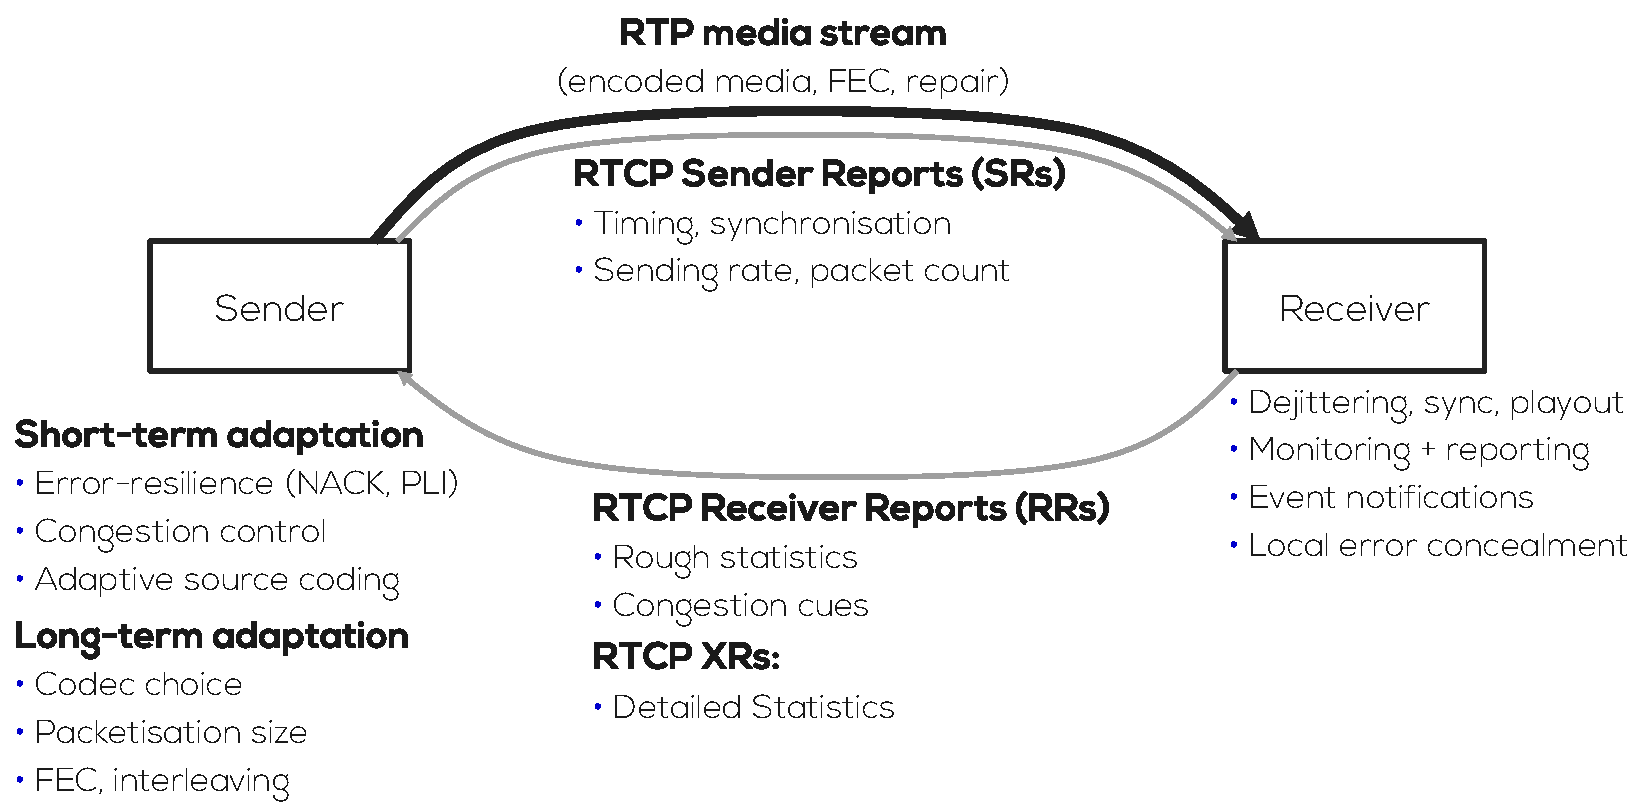
\includegraphics[width=\textwidth]{chap3-fig-rtp-rtcp}
}
\caption{RTP and RTCP for adaptive real-time applications.{\scriptsize Source:
J\"org Ott, ``Networked Multimedia Protocols and Systems''}.}
\label{fig:3:rtp:model}
\end{figure}

Figure~\ref{fig:3:rtp.hdr} describes the RTP packet header format. The
\textit{synchronization source} (SSRC) assists in determining the source
endpoint, typically useful when an endpoint sends multiple media streams that
need to be synchronized (e.g., audio and video lip-sync). The \textit{RTP
timestamp} assists in playing out the received packets at the appropriate
instance of time and recomposing the media frame from RTP packets. The
\textit{RTP sequence number} assists in identifying the lost packets and 
re-ordering packets in the case of out-of-order packet arrival. Lastly, RTP uses
the \textit{`payload type'} (PT) to describe the encoding of the media data it is
carrying. Consequently, each codec needs to specify its corresponding payload
format.

% \begin{figure}[!h]
% \centerline{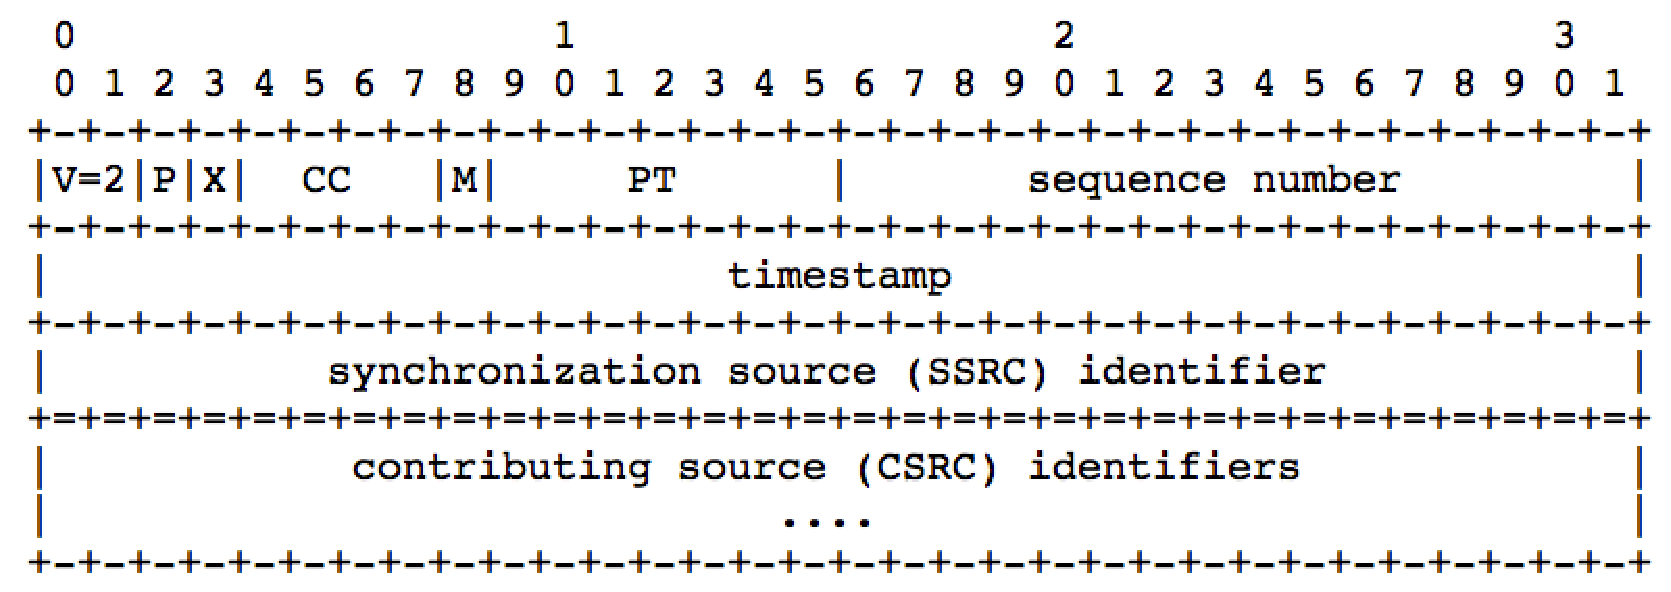
\includegraphics[width=\textwidth]{chap3_fig_hdr_rtp}}
% \caption{shows the RTP packet format that encapsulates the media data.}
% \label{fig:3:rtp.hdr}
% \end{figure}

\begin{figure}[!h]
\begin{spacing}{0.5}
\centering
{\small
\begin{verbatim}
    0                   1                   2                   3
    0 1 2 3 4 5 6 7 8 9 0 1 2 3 4 5 6 7 8 9 0 1 2 3 4 5 6 7 8 9 0 1
   +-+-+-+-+-+-+-+-+-+-+-+-+-+-+-+-+-+-+-+-+-+-+-+-+-+-+-+-+-+-+-+-+
   |V=2|P|X|  CC   |M|     PT      |       sequence number         |
   +-+-+-+-+-+-+-+-+-+-+-+-+-+-+-+-+-+-+-+-+-+-+-+-+-+-+-+-+-+-+-+-+
   |                           timestamp                           |
   +-+-+-+-+-+-+-+-+-+-+-+-+-+-+-+-+-+-+-+-+-+-+-+-+-+-+-+-+-+-+-+-+
   |           synchronization source (SSRC) identifier            |
   +=+=+=+=+=+=+=+=+=+=+=+=+=+=+=+=+=+=+=+=+=+=+=+=+=+=+=+=+=+=+=+=+
   |            contributing source (CSRC) identifiers             |
   |                             ....                              |
   +-+-+-+-+-+-+-+-+-+-+-+-+-+-+-+-+-+-+-+-+-+-+-+-+-+-+-+-+-+-+-+-+
\end{verbatim}
}
\end{spacing}
\caption{The RTP packet format that encapsulates the media data.}
\label{fig:3:rtp.hdr}
\end{figure}


\begin{figure}[!h]
\begin{spacing}{0.5}
{\footnotesize
\begin{verbatim}
          0                   1                   2                   3
          0 1 2 3 4 5 6 7 8 9 0 1 2 3 4 5 6 7 8 9 0 1 2 3 4 5 6 7 8 9 0 1
         +-+-+-+-+-+-+-+-+-+-+-+-+-+-+-+-+-+-+-+-+-+-+-+-+-+-+-+-+-+-+-+-+
  header |V=2|P|    RC   |   PT=SR=200   |             length            |
         +-+-+-+-+-+-+-+-+-+-+-+-+-+-+-+-+-+-+-+-+-+-+-+-+-+-+-+-+-+-+-+-+
         |                         SSRC of sender                        |
         +=+=+=+=+=+=+=+=+=+=+=+=+=+=+=+=+=+=+=+=+=+=+=+=+=+=+=+=+=+=+=+=+
  sender |              NTP timestamp, most significant word             |
  info   +-+-+-+-+-+-+-+-+-+-+-+-+-+-+-+-+-+-+-+-+-+-+-+-+-+-+-+-+-+-+-+-+
         |             NTP timestamp, least significant word             |
         +-+-+-+-+-+-+-+-+-+-+-+-+-+-+-+-+-+-+-+-+-+-+-+-+-+-+-+-+-+-+-+-+
         |                         RTP timestamp                         |
         +-+-+-+-+-+-+-+-+-+-+-+-+-+-+-+-+-+-+-+-+-+-+-+-+-+-+-+-+-+-+-+-+
         |                     sender's packet count                     |
         +-+-+-+-+-+-+-+-+-+-+-+-+-+-+-+-+-+-+-+-+-+-+-+-+-+-+-+-+-+-+-+-+
         |                      sender's octet count                     |
         +=+=+=+=+=+=+=+=+=+=+=+=+=+=+=+=+=+=+=+=+=+=+=+=+=+=+=+=+=+=+=+=+
  report |                 SSRC_1 (SSRC of first source)                 |
  block  +-+-+-+-+-+-+-+-+-+-+-+-+-+-+-+-+-+-+-+-+-+-+-+-+-+-+-+-+-+-+-+-+
    1    | fraction lost |       cumulative number of packets lost       |
         +-+-+-+-+-+-+-+-+-+-+-+-+-+-+-+-+-+-+-+-+-+-+-+-+-+-+-+-+-+-+-+-+
         |           extended highest sequence number received           |
         +-+-+-+-+-+-+-+-+-+-+-+-+-+-+-+-+-+-+-+-+-+-+-+-+-+-+-+-+-+-+-+-+
         |                      interarrival jitter                      |
         +-+-+-+-+-+-+-+-+-+-+-+-+-+-+-+-+-+-+-+-+-+-+-+-+-+-+-+-+-+-+-+-+
         |                         last SR (LSR)                         |
         +-+-+-+-+-+-+-+-+-+-+-+-+-+-+-+-+-+-+-+-+-+-+-+-+-+-+-+-+-+-+-+-+
         |                   delay since last SR (DLSR)                  |
         +=+=+=+=+=+=+=+=+=+=+=+=+=+=+=+=+=+=+=+=+=+=+=+=+=+=+=+=+=+=+=+=+
  report |                 SSRC_2 (SSRC of second source)                |
  block  +-+-+-+-+-+-+-+-+-+-+-+-+-+-+-+-+-+-+-+-+-+-+-+-+-+-+-+-+-+-+-+-+
    2    :                               ...                             :
         +=+=+=+=+=+=+=+=+=+=+=+=+=+=+=+=+=+=+=+=+=+=+=+=+=+=+=+=+=+=+=+=+
         |                  profile-specific extensions                  |
         +-+-+-+-+-+-+-+-+-+-+-+-+-+-+-+-+-+-+-+-+-+-+-+-+-+-+-+-+-+-+-+-+
\end{verbatim}
}
\end{spacing}
\caption{The RTCP packet format for carrying the Sender Report (SR) and
the Receiver Report (RR). The SR carries transport statistics and enables 
stream synchronization, while the RR carries the receiver transport 
characteristics.}
\label{fig:3:rtcp.hdr}
\end{figure}

% \begin{figure}[!h]
% \centering{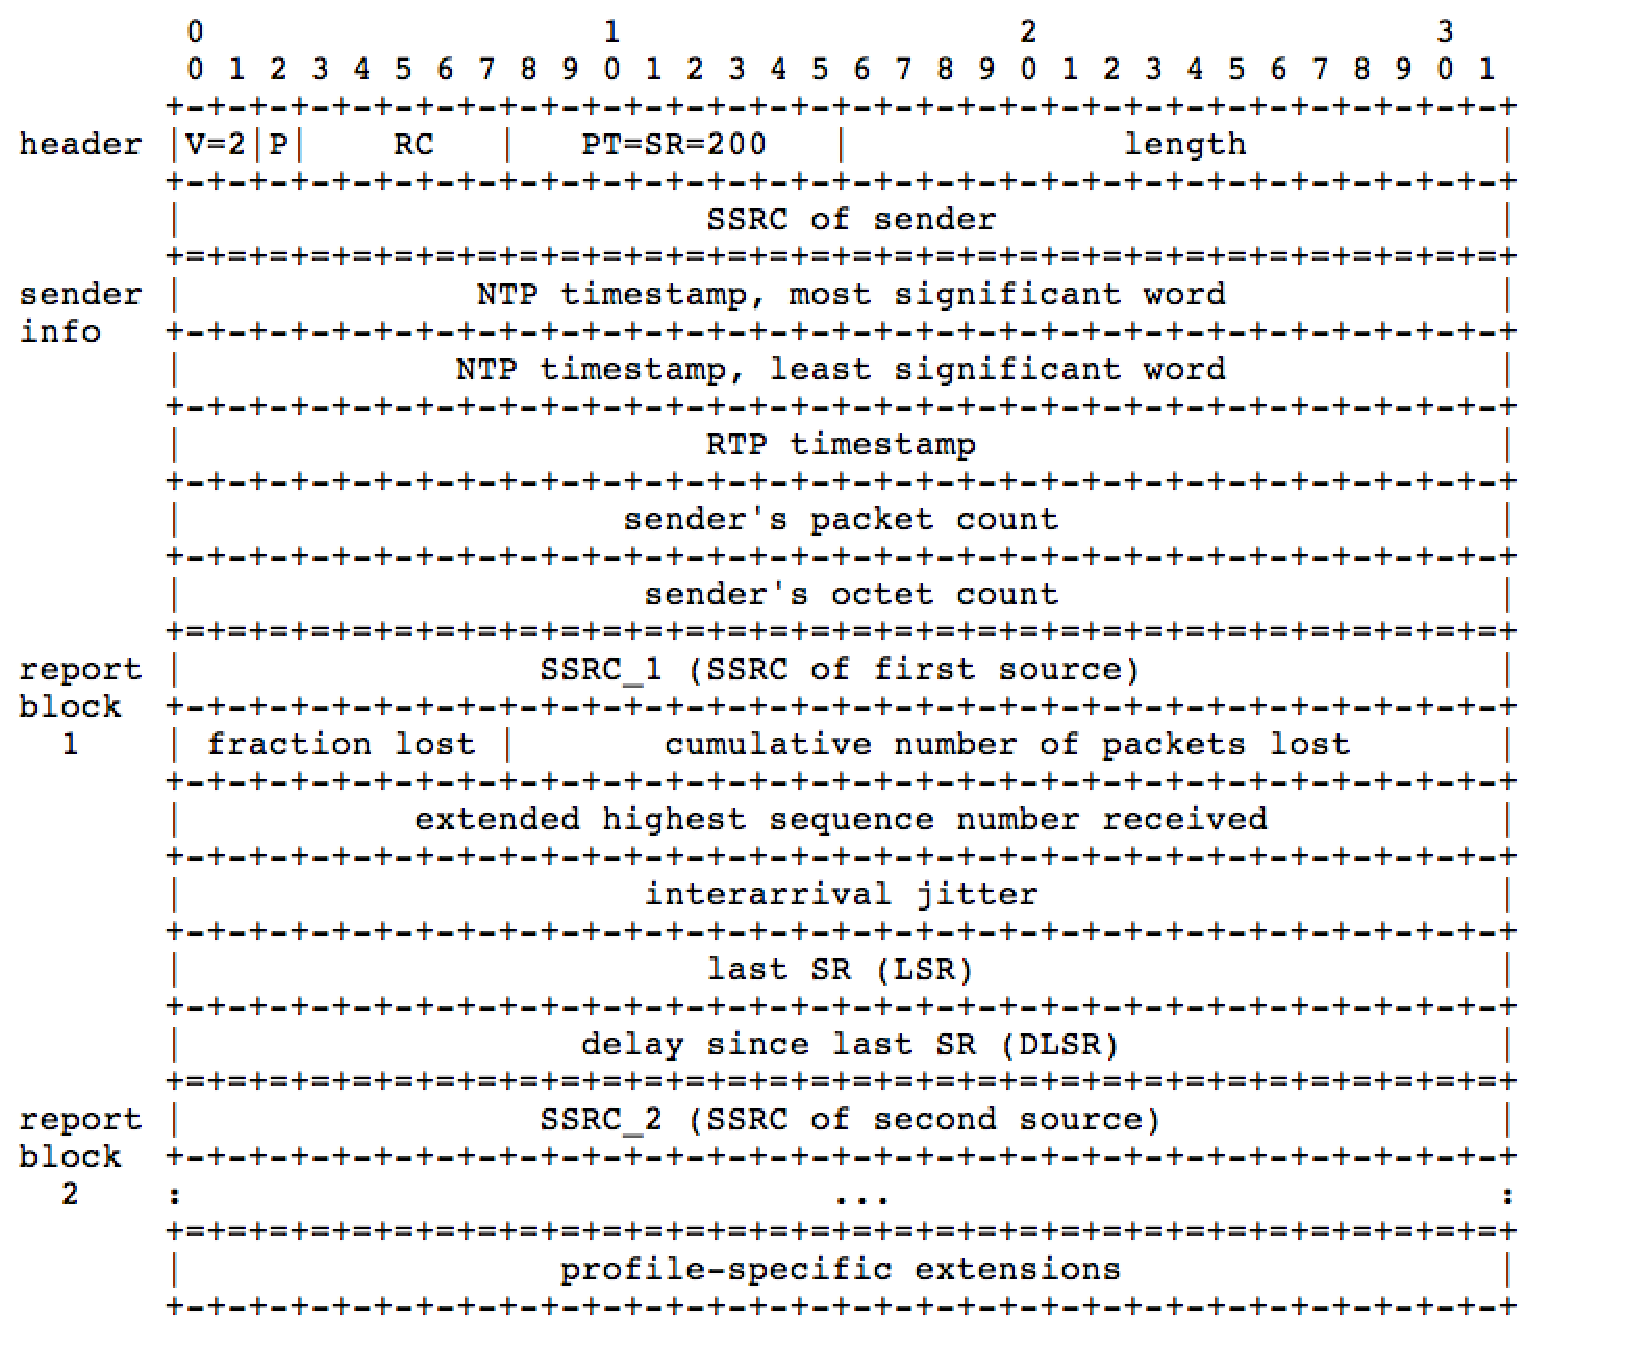
\includegraphics[width=\textwidth]{chap3_fig_hdr_rtcp}}
% \caption{shows the RTCP packet format for carrying the Sender Report (SR) and
% the Receiver Report (RR). The SR carries transport statistics and enables 
% stream synchronization, while the RR carries the receiver transport 
% characteristics.}
% \label{fig:3:rtcp.hdr}
% \end{figure}

The receiver measures the incoming streams and reports the coarse-grained
transport statistics in an RTCP Receiver Report (RR). The RTCP RR contains the
current loss fraction, jitter, and the highest sequence number received, and it
facilitates in calculating the round-trip time (RTT). The sender uses RTCP Sender Reports (SRs)
to assist in synchronizing the media streams (audio and video) by relating the
RTP timestamps of the individual media streams to the wall clock time (NTP)
and notifying the receiver about the current packet rate and bit rate.
Figure~\ref{fig:3:rtcp.hdr} shows the RTCP packet header format for a
interactive unicast media stream (i.e., both sending and receiving media).

\section{RTP Payload Formats}

The general principle for defining payload formats/types is to 
identify the encoding of the media packets. These encodings are either  
codec-specific (e.g., H.264, H.263, H.261, MPEG-2, JPEG, G.711, G.722, AMR, etc.),
or generic (e.g., Forward Error Correction (FEC), NACK, multiplexed streams).
Typically, a payload document specifies a well-defined packet format for media
codecs; it also defines \emph{aggregation rules} for codecs that produce
several small frames (e.g., audio) compared to the IP Maximum Transmission
Unit (MTU), and \emph{fragmentation rules} for codecs that produce large frames
(e.g., I-frames by video codecs). The main reason for fragmenting large
frames into smaller packets and not rely on IP fragmentation is that IP
fragmented packets are commonly discarded in the network, especially by NATs
or firewalls.

% Usually the RTP header is immediately followed by
% payload-specific header (payload format) and then by the media data. This
% allows the sending endpoint to semantically fragment large packets, which
% simplifies processing and decoding at the receiver (i.e., be able to decode
% individual packets without relying on receiving other packets).

\begin{figure}[!h]
\begin{spacing}{0.5}
{\footnotesize
\begin{verbatim}
    0                   1                   2                   3
    0 1 2 3 4 5 6 7 8 9 0 1 2 3 4 5 6 7 8 9 0 1 2 3 4 5 6 7 8 9 0 1
   +-+-+-+-+-+-+-+-+-+-+-+-+-+-+-+-+-+-+-+-+-+-+-+-+-+-+-+-+-+-+-+-+
   |V=2|P|X|  CC   |M|     PT      |       sequence number         |
   +-+-+-+-+-+-+-+-+-+-+-+-+-+-+-+-+-+-+-+-+-+-+-+-+-+-+-+-+-+-+-+-+
   |                           timestamp                           |
   +-+-+-+-+-+-+-+-+-+-+-+-+-+-+-+-+-+-+-+-+-+-+-+-+-+-+-+-+-+-+-+-+
   |           synchronization source (SSRC) identifier            |
   +=+=+=+=+=+=+=+=+=+=+=+=+=+=+=+=+=+=+=+=+=+=+=+=+=+=+=+=+=+=+=+=+
   |                 Payload Format-Specific Header                |
   +               +-+-+-+-+-+-+-+-+-+-+-+-+-+-+-+-+-+-+-+-+-+-+-+-+
   |               |                                               |
   +-+-+-+-+-+-+-+-+                                               +
   |                           Media Data                          |
   +                                                               +
   |                                                               |
   +-+-+-+-+-+-+-+-+-+-+-+-+-+-+-+-+-+-+-+-+-+-+-+-+-+-+-+-+-+-+-+-+
\end{verbatim}
}
\end{spacing}
\caption{Packet structure of an RTP packet encapsulating the
payload-specific header and the associated media data.}
\label{fig:3:pt.fmt}
\end{figure}

% \begin{figure}[!t]
% \centerline{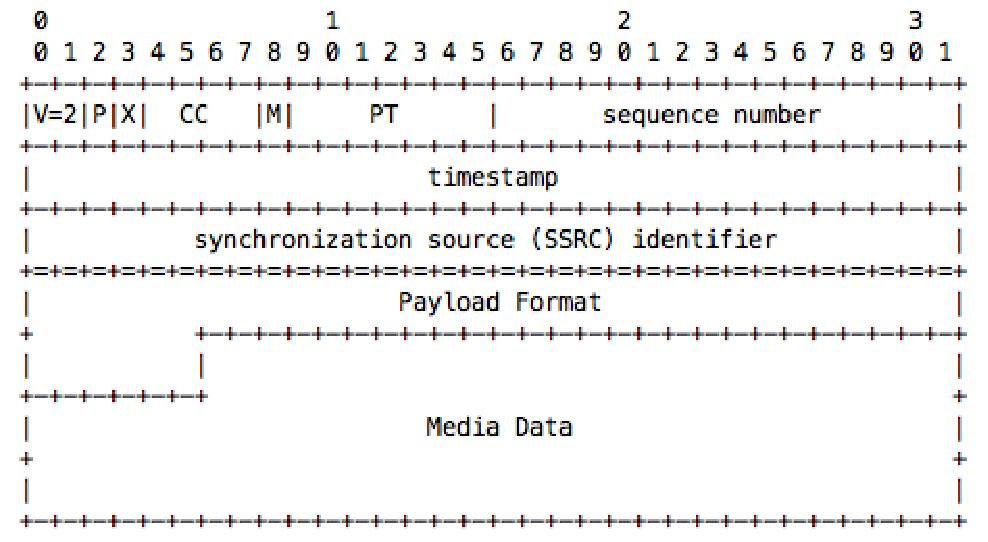
\includegraphics[width=\textwidth]{chap3_fig_hdr_pt_fmt}}
% \caption{shows the packet structure of an RTP packet encapsulating the
% payload-specific header and the associated media data.}
% \label{fig:3:pt.fmt}
% \end{figure}

\section{RTP Header Extensions}

RTP header extensions carry media-independent information, i.e., data that may
be generically applicable to multiple payload formats (e.g., timing
information), and needs to be reported more frequently than RTCP reports are
emitted. A commonly-cited example is the sending of NACK packets for interactive video,
where media flows in both directions and RTP packets are generated every tens
of milliseconds. In this case, the RTP header extension can indicate which sequence numbers
were correctly received or lost, thereby not completely relying on the RTCP
receiver reports to send NACKs or ACKs.

The advantage of using header extensions is that they are backwards
compatible, i.e., an endpoint that does not understand them is able ignore
them. Some current use-cases for RTP header extensions include reporting the
network send timestamp: instead of bursting packets from a large frame on to
the network, the sender paces these packets.  Another example is equalizing a
client's audio levels across multiple streams in a video conference. Lastly,
RTP header extensions are generic, there is no need to redefine the same extension
for each media codec.

\section{RTCP Reporting Interval}
% timing

A closed control loop is formed by sending RTP media packets and receiving
RTCP feedback packets. The RTCP feedback interval is typically limited to a
small fraction of the session bandwidth (\emph{session\_bw}) as not to affect the media traffic.
The RTCP reporting interval is determined by the number of SSRCs in the
session (denoting the session size), and the chosen session bandwidth. The
session bandwidth (\emph{session\_bw}) is expected to be divided amongst the participants, but
oftentimes it is calculated as the sum of the average throughput of the
senders expected to be concurrently active. In the case of an audio conference,
the session bandwidth would be one sender's bandwidth, but for a video
conference, the session bandwidth would vary depending on the number of participants displayed on
the user interface. Consequently, the session bandwidth is supplied by the
session management layer so that the same value for the RTCP interval is calculated for each participant.


The recommended fraction of the session bandwidth allocated for control
traffic is 5\,\%. For many scenarios, including large conferences, where there
are a large number of receivers but a small number of senders, it is
recommended that a quarter of the reporting bandwidth (\emph{rtcp\_bw}) be
shared equally by the senders and the remaining three-quarters by the receivers. The
main reason for this allocation ratio is to allow newly-joining participants to quickly receive the
CNAME and synchronization timestamps from the Sender Reports (SRs). 
For new participants (even if they are just receivers), the RTCP
interval is halved to quickly declare their presence.  Lastly, the recommended
value for a fixed minimum RTCP interval is 5 seconds, while the value for a
reduced minimum is $\frac{360}{session\_bw}s$.  The fixed minimum RTCP
interval of \emph{5\,s} is suitable for unidirectional links or for sessions
that do not require monitoring of the reception quality statistics (e.g., IPTV),
while the reduced minimum RTCP interval is also suitable for participants in a
unicast bidirectional multimedia session. The reduced minimum RTCP interval
is suitable for sending timely feedback messages to either perform congestion
control or error repair; the interval is shorter than \emph{5\,s} for session
bandwidths greater than \emph{72\,kbps}.

% avpf

If an endpoint detects packet loss or the onset of congestion midway through a
reporting interval, the base RTP specification~\cite{rfc3550} (AVP profile)
does not allow the RTCP reports to be sent early and the endpoint has to wait for
the next scheduled RTCP report. In this case, the slow control loop causes
instability and oscillation in the media bit rate. To overcome this
shortcoming, endpoints implement the Extended RTP Profile for RTCP-Based
Feedback (AVPF profile)~\cite{rfc4585}, an extension to RTP's default timing
rules, to enable rapid feedback. This profile allows the endpoint to adjust the
RTCP reporting interval to send the RTCP feedback reports earlier than the
next scheduled RTCP report, sometimes even immediately, as long as the reporting
interval on average remains the same. Figure~\ref{fig:3:avpf.interval} shows
that with AVP profile, the endpoint reports at regular intervals, whereas with AVPF
the endpoint it gets the opportunity to send feedback early in every other reporting
interval. Along with the possibility of providing timely feedback, the AVPF
profile also defines a suite of error-resilience feedback messages, namely,
Negative Acknowledgments (NACK), Picture Loss Indication (PLI), Slice Loss
Indication (SLI), and the Reference Picture Selection Indication (RPSI).

\begin{figure}[!t]
\centering{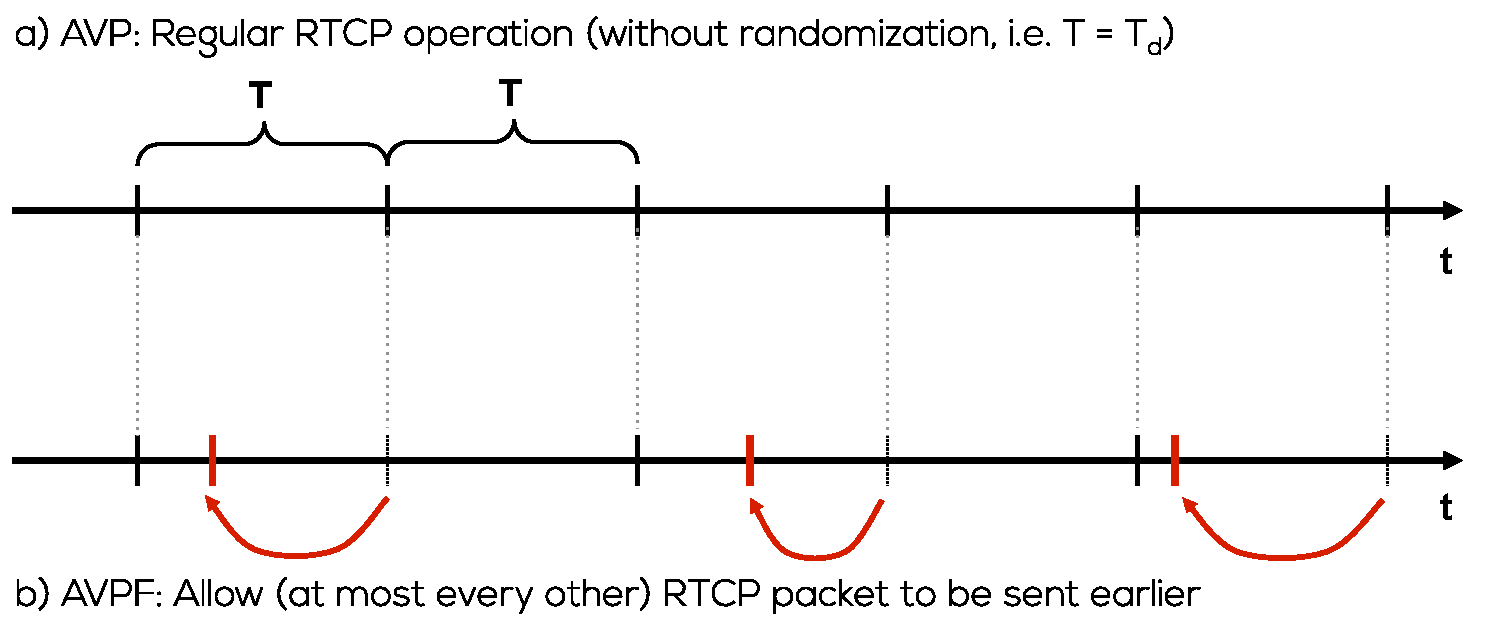
\includegraphics[width=\textwidth]{chap3-fig-avpf-rtcp}}
\caption{The RTCP reporting interval as defined in a) AVP, b) AVPF.}
\label{fig:3:avpf.interval}
\end{figure}




\section{RTCP Extended Reports (XRs) for Performance Monitoring}

Endpoints use RTCP Extended Reports (XRs)~\cite{rfc3611} to describe complex
metrics that are not exposed by the RTCP Receiver Report (RR). Some examples of
XRs relevant to performance monitoring and congestion control are: de-jitter
buffer metrics~\cite{rfc7005}, Packet Delay Variation (PDV)~\cite{rfc6798},
delay metrics~\cite{rfc6843}, burst-gap discard~\cite{rfc7003}, burst-gap
loss~\cite{rfc6958}, Run-Length Encoded (RLE) loss~\cite{rfc3611}, discard
RLE~\cite{rfc7097}, the number of discarded packets~\cite{rfc7002} and
bytes~\cite{rfc7243}, summary statistics~\cite{rfc7004},
Quality of Experience (QoE)~\cite{draft.xr.qoe}, and loss
concealment~\cite{draft.xr.conceal}, etc. RTP allows for new metrics to be
defined; the main requirement is to document what is measured, how it is
measured and how it is reported to the other endpoints.


% The RTCP Extended Reports (XR) [RFC3611] allow reporting of more
% complex and sophisticated reception quality metrics, but do not
% change the RTCP timing rules.  RTCP extended reports of potential
% interest for congestion control purposes are the extended packet
% loss, discard, and burst metrics [RFC3611],
% [I-D.ietf-xrblock-rtcp-xr-discard],
% [I-D.ietf-xrblock-rtcp-xr-discard-rle-metrics],
% [I-D.ietf-xrblock-rtcp-xr-burst-gap-discard],
% [I-D.ietf-xrblock-rtcp-xr-burst-gap-loss]; and the extended delay
% metrics [RFC6843], [RFC6798].


\section{Codec Control Messages}
% codec control

Sometimes an endpoint needs to configure or notify the other endpoint's codec.
These messages are broadly classified as \emph{Transport Layer} and \emph
{Payload-specific} feedback messages~\cite{rfc4585, rfc5104}. The transport
layer messages are: Temporary Maximum Media Stream Bit Rate Request (TMMBR)
and Temporary Maximum Media Stream Bit Rate Notification (TMMBN). The
receiving endpoint uses the TMMBR message to configure the maximum encoding
bit rate of the media stream, while the sending endpoint uses the TMMBN to
inform the receiver of the updated bit rate. Therefore, transport layer
feedback messages are intended to transmit general purpose feedback messages,
independent of any particular codec or application.

On the other hand, the payload-specific feedback messages carry information
specific to a certain payload type and are acted upon by the codec layer. Some
examples of these type of messages are: Full Intra Request (FIR), 
temporal-spatial tradeoff, frame rate, frame size, maximum packet size or packet rate,
etc.~\cite{draft.avt.cop}.

\section{Reduced-Size RTCP Reports}
% non-compound feedback

An endpoint sends RTCP feedback as a \emph{compound}, or \emph{minimal}, RTCP
packet. A \emph{compound RTCP packet} as defined in~\cite{rfc3585} contains
at least a sender report (SR) or a receiver report (RR) or both, followed by
a Source Description (SDES) and any additional XR blocks. A \emph{minimal RTCP
packet} is one that contains an SR and/or RR, and is followed by an SDES
containing just the canonical name (CNAME)\footnote{The real name
(identifier) used to describe the source; it can be in any form desired by the
user. Of the SDES items (username, email, phone, geolocation, etc.), it is 
compulsory to include CNAME in every RTCP packet.}. Hence, every compound RTCP
packet is a minimal RTCP packet with additional report blocks. A typical RTCP
packet size for conversational multimedia streams is 80 bytes (RTCP=8, SR=20,
RR=24, SDES/CNAME =28).

Including any of the additional SDES items or adding XR blocks makes the
compound RTCP packet very large. On low bit rate links, these large compound
RTCP packets may introduce more delay. Therefore, it may be desirable to
logically fragment the report blocks in a compound RTCP packet and send them
independently. These fragmented report blocks are called \emph {reduced-size
RTCP packets}~\cite{rfc5506}. Unlike compound RTCP packets, to transmit a
reduced-size RTCP packet an endpoint does not need to include the minimal RTCP
report. However, when using reduced-size RTCP packets, minimal packets need to
be sent once in a while to keep the CNAME-SSRC binding alive.

Reduced-size RTCP reports are beneficial in wireless networks where the packet
loss rate increases with the packet size, i.e., larger-sized packets are more
susceptible to being dropped compared with smaller-sized packets. Additionally, smaller
packets have shorter serialization time, i.e., the amount of time it takes for
the endpoint to put the data packet onto the link is short.

The main reasons for the application to use reduced-size RTCP reports are:
1) to notify the other endpoint of events. Using the signaling channel would
incur at least one RTT while implementing it as an RTCP extension would merely
incur a one-way delay. 2) to send codec control (e.g., TMMBR) or feedback (e.g.,
NACK, RPSI) messages. These reduced-size messages are more likely to be
transmitted more often and with as little delay as possible, especially since
these types of messages are more likely to be sent when link conditions are
poor.


% relationship with SDP
\section{Session Setup}

% SDP O/A, declarative SDP, RTCP notify

There are several ways to set up an interactive or conversational multimedia
session, for example by implementing one of the following: H.323~\cite{H.323},
Session Initiation Protocol (SIP)~\cite{rfc3261}, or Jingle~\cite{XEP-0166}, an
extension to the Extensible Messaging and Presence Protocol
(XMPP)~\cite{rfc6120}.

SIP uses the Session Description Protocol (SDP)~\cite{rfc4566} to describe the
endpoint's transport and media capabilities. An SDP description defines a
single multimedia session, i.e., an association between a set of participants.
It may, however, carry multiple media streams in the session.

\begin{figure}[!h]
\centerline{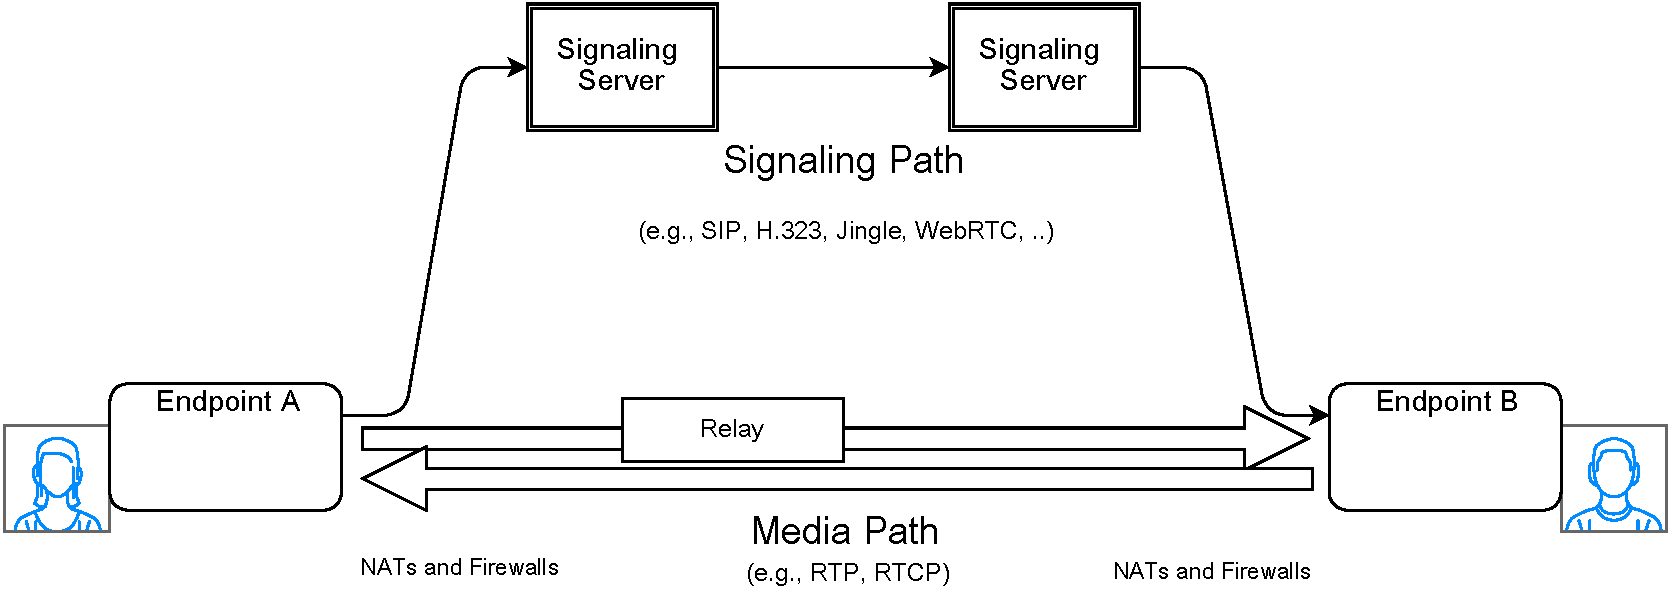
\includegraphics[width=\textwidth]{chap3-fig-sig-med}}
\caption{The signaling and media paths between two endpoints engaging in
a video call.}
\label{fig:3:sig.media}
\end{figure}


The transport details in the SDP are mainly split into two parts: the protocol
for delivering media packets (currently, TCP, UDP, or SCTP), and the 
IP address of the endpoint. The protocol to deliver the media packets is
chosen by the application, but identifying the IP address and port of an
endpoint is a bit complex. It first requires gathering the endpoint's multiple
IP addresses and later exchanging them with the other endpoints to establish
connectivity.

Multiple IP addresses arise not only from multiple interfaces but also from
the presence of NAT devices in the network, which may change the IP address of
the outgoing packets. Since interactive media calls are between endpoints and
media streams may eventually traverse a NAT at both ends, in some cases, the
only way to deliver media packets between two endpoints would is by using
a relay\footnote{Traversal Using Relays around NAT (TURN)} on the public
Internet. Hence, the endpoint needs to discover its 2-tuple \texttt{[IP
address:port]} on the host, which is relatively easy followed by the public 
address, if behind a NAT~\cite{rfc5389}. Discovering an endpoint's public address
requires contacting a publicly-hosted STUN\footnote{Session Traversal
Utilities for NAT (STUN).} server and comparing the endpoint's
host addresses with the one observed by the STUN server. Lastly, the endpoint
discovers the address allocated by the TURN relay~\cite{rfc5766} and notifies
the other endpoints about its transport details. This collection of 2-tuples
is known as \emph{candidates}. First, each endpoint sorts its candidates
in decreasing order of priority and exchanges these candidate addresses in the
SDP with the other endpoint. On receiving the list of candidates, the endpoints
probes between each combination of addresses in the two candidate
lists; a pair of addresses is called a \emph{candidate pair}. The endpoint
chooses the first candidate pair that successfully establishes connectivity
(\emph{aggressive nomination}). This process of performing pair-wise
\emph{connectivity checks} is called Interactive Connectivity Establishment
(ICE)~\cite{rfc5245, rfc6544} and it relies on the STUN protocol~\cite{rfc5389} to establish connectivity
across a NAT. In case direct connectivity between the two endpoints fails 
to be established, the individual endpoints use the \emph{Traversal Using Relays
around NAT} (TURN) server and the associated protocol~\cite{rfc5766} to relay
media packets between them. Similar to the STUN server, the TURN
server is hosted on the public Internet.

% Depending on the type of NAT device (full-cone, address- or port-restricted
% cone, symmetric).

\begin{figure}[!h]
{\small
\begin{verbatim}
        v=0
        o=jdoe 2890844526 2890842807 IN IP4 10.0.1.1
        s=
        c=IN IP4 192.0.2.3
        t=0 0
        a=ice-pwd:asd88fgpdd777uzjYhagZg
        a=ice-ufrag:8hhY
        m=audio 45664 RTP/AVP 0
        a=rtpmap:0 PCMU/8000
        a=candidate:1 1 UDP 2130706431 10.0.1.1 8998 typ host
        a=candidate:2 1 UDP 1694498815 195.148.127.98 45664 typ srflx 
            raddr 10.0.1.1 rport 8998
\end{verbatim}
}
\caption{Sample SDP containing the sender's transport and media capabilities.}
\label{fig:3:sdp}
\end{figure}

The second part of SDP carries the media capabilities, together with the 
transport parameters, that bind the SDP to the Offer/Answer model. In the O/A
model, the sending endpoint \emph{offers} to the receiver a set of media
capabilities in decreasing order of preference, typically, multiple options of
audio/video codecs and ICE candidates. On receiving the sender's capabilities,
the receiver compares its media capabilities with the sender's and responds
with the one that best fits the receiver's requirements (\emph{answer}). The
\emph{offer is rejected} if the receiver is unable to pick any
of the options provided by the sender, or if the ICE connectivity checks fail.
Hence, the application at the sender needs to pick a minimum number of widely-available 
audio and video codecs to avoid negotiation failure. If the
\emph{offer is accepted}, both endpoints then know the following: 1) which
audio and/or video codecs to use, 2) the payload types of the encoded media
streams (possibly even their respective SSRCs), 3) to which IP address and
port number to send the media stream, 4) the media session bandwidth, if
indicated, and 5) the encryption keys, if encrypting traffic.

\begin{figure}
\centering{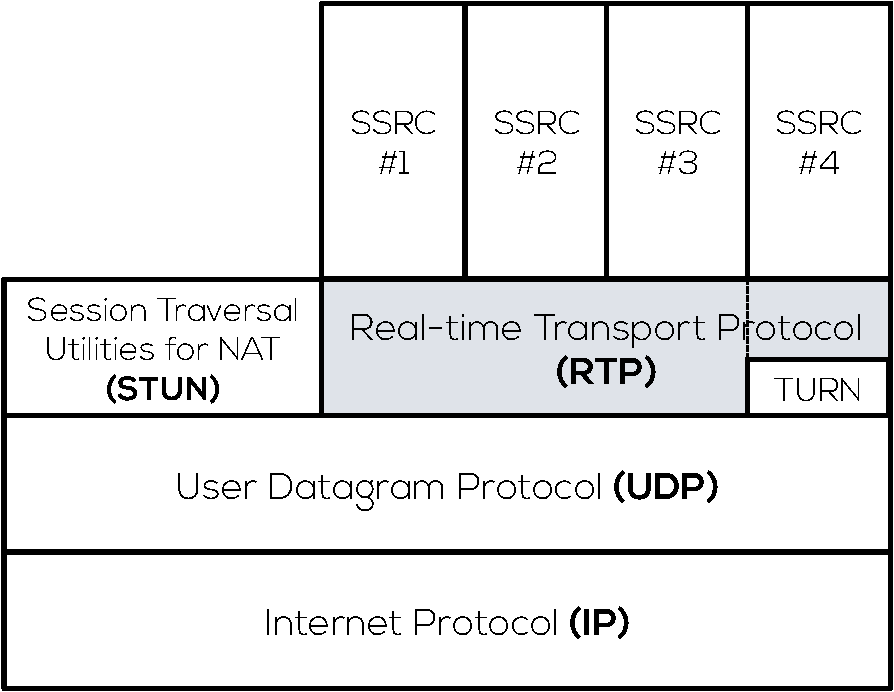
\includegraphics[width=0.9\textwidth]{chap3-fig-rtp-stack}}
\caption{Relationship of RTP with STUN, TURN, DTLS and the signaling protocol.}
\label{fig:3:rtp-stack}
\end{figure}

Figure~\ref{fig:3:rtp-stack} shows the relationship of the RTP stack with the
rest of the IP stack. RTP is usually transmitted over UDP, but under some
constrained situations (e.g., restrictive firewalls or NATs), RTP may be
encapsulated in TCP~\cite{rfc3550}. STUN~\cite{rfc5389} is used by ICE to
discover the presence of a NAT device and obtain the mapped (public) IP
address. When using a TURN relay server (in the presence of symmetric NATs or
when concealing the host address of the caller for privacy reasons), the RTP
packets are encapsulated inside the TURN's \emph{ChannelData}
message~\cite{rfc5766}. In Figure~\ref{fig:3:rtp-stack}, four media streams
(SSRC \#1-4) are transmitted by RTP over UDP, but two streams (SSRC \#1-2) are
relayed through a TURN server. Secure RTP (SRTP)~\cite{rfc3611} is a security
framework that provides confidentiality by encrypting RTP payload (not the RTP
headers) and supports source origin authentication. While SRTP is not the only
security mechanism for RTP~\cite{draft.srtp-not-must}, it is widely
applicable, especially to voice telephony and group communication. However,
the main challenge for SRTP is key management~\cite{draft.sec-opts}, since
many options exist (e.g., SRTP over DTLS in WebRTC~\cite{rfc5763}, MIKEY in
SIP~\cite{rfc3830}, Security Description in SDP~\cite{rfc4566},
ZRTP~\cite{RFC6189}, etc.).

\section{Summary}

In this chapter we introduced the basic features of RTP and RTCP; we discussed
the limits on reporting interval and the numerous RTP and RTCP extensions.
The introduction to RTP and RTCP largely provides context and helps understand
the design constraints  for multimedia congestion control which are discussed 
in more detail in the forthcoming chapters.


\chapter{Congestion Control Framework for Real-time Communication}
\label{chap:cc.fw}
In the forthcoming deployment of WebRTC systems, we speculate that high
quality\footnote{normally, high quality corresponds to an increase in required
bandwidth.} video conferencing will see wide-scale adoption. To assure
stability of the network (and avoid congestion collapse), these real-time
communication systems are required to implement some kind of congestion
control for their RTP-based media traffic.

RTP transmits the media data over IP using a variety of transport layer
protocols such as UDP, TCP, and Datagram Congestion Control Protocol (DCCP).
Consequently, congestion control for RTP-based media flows is implemented
either in the application or the media flows are transmitted over
congestion-controlled transport (TCP or DCCP). While using a congestion-controlled 
transport may be safe for the network, it is sub-optimal for the
media quality unless the congestion-controlled transport is designed to carry
media flows. Unfortunately, TCP is only suitable for interactive multimedia
for paths with very low RTT (<100\,\emph{ms} )~\cite{Brosh:tcp-real-time}, and
DCCP packets have problems with NAT traversal~\cite{schier:DCCP} unless DCCP is
encapsulated in UDP~\cite{RFC6773}.

This motivates the need for a UDP congestion control algorithm, where the
congestion control is implemented between the application and the
underlying transport, thereby taking into
account both the application's and the transport's requirements or constraints
and with appropriate trade-off. In this thesis, we consider congestion
control for unicast RTP traffic running over the best-effort IP network.

% CC should not cause queuing delay. Or define low-latency operation of
% multimedia cc.

Endpoints rely on RTCP feedback from the receiver to implement congestion
control. Hence, the congestion control should consider the following three aspects
in its design: congestion cues to report, block size of each report or the
overhead incurred by reporting a cue, and the frequency of these feedback
reports. In the following subsections, we describe the interaction between the
application and the congestion control, list common congestion cues, discuss
the feedback reporting frequency, the classification of cues, the metrics and
criteria to evaluate congestion control proposals, and lastly, we discuss the
RTP circuit breaker which stops transmission permanently after observing
prolonged congestion.

\section{Adaptive Multimedia Systems}
\label{fw.amusys}

Any real-time communication endpoint is made up of three basic components:
codec (encoder and decoder), transport (RTP and UDP) and the application
preferences (user and application settings, system policies, capturing and
rendering constraints, etc.). The codec encodes and decodes a media stream. A
typical application comes with at least one codec each for audio and video. 
The application may also implement several other media codecs so that 
it is capable of inter-operating
with several different types of endpoints. The transport is mainly made up of
RTP, which packetizes and depacketizes the media and UDP to transmit the
media. The application preferences are made up of system polices (which
interface to use? which codec to prefer?), codec settings (the
preferred or the minimum video resolution, preferred frame rate, etc.). The
application preferences may also depend on the outcome of the session
establishment, in which the participating endpoints negotiate the codec and
network settings.

\begin{figure}
  \centerline{
    \subfloat[Sending Endpoint]{
      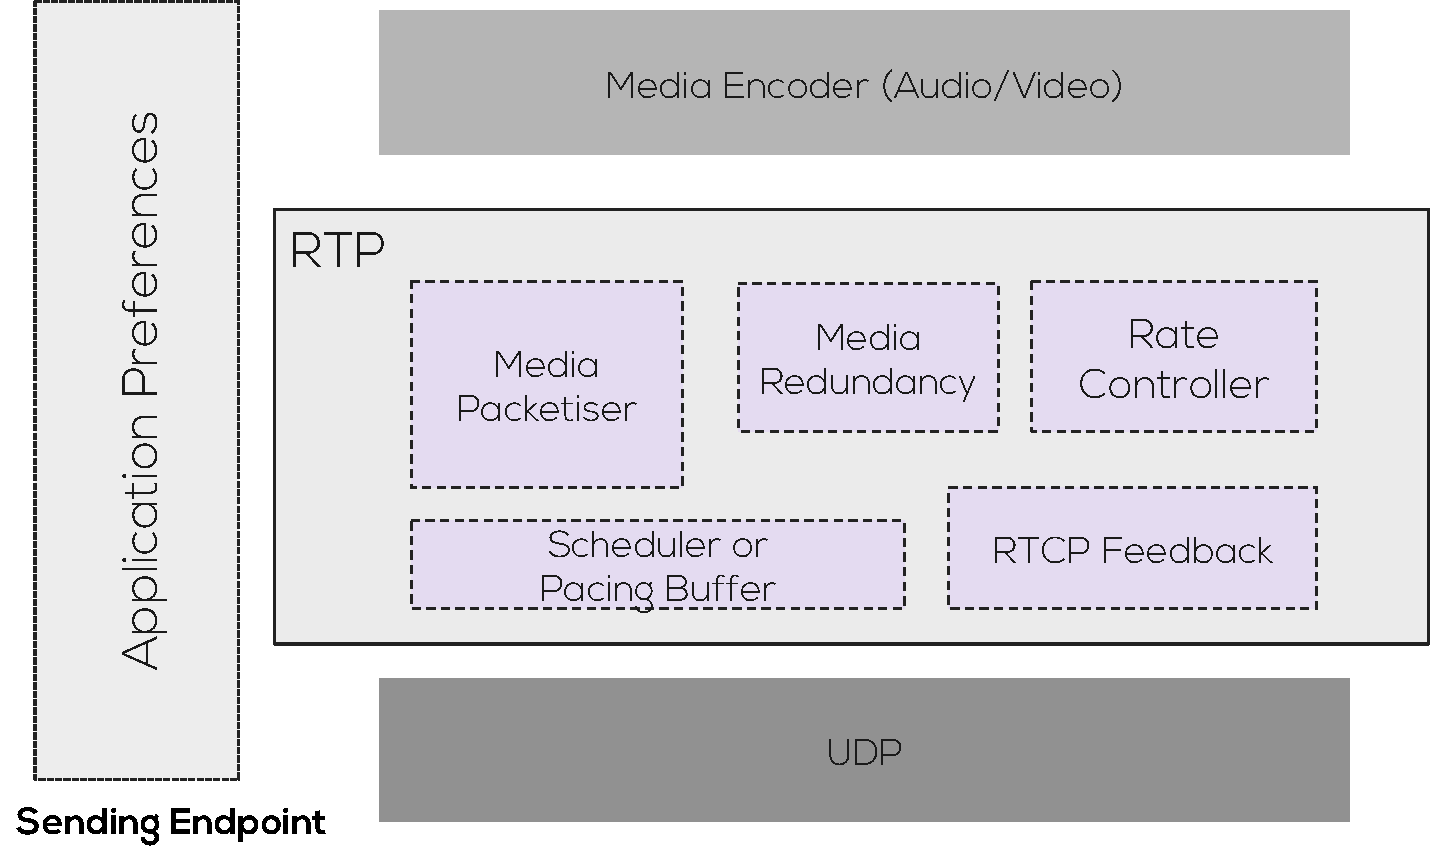
\includegraphics[width=0.66\textwidth]
      {chap4_fig_app_sender}
    }
  }
  \centerline{
    \subfloat[Receiving Endpoint]{
      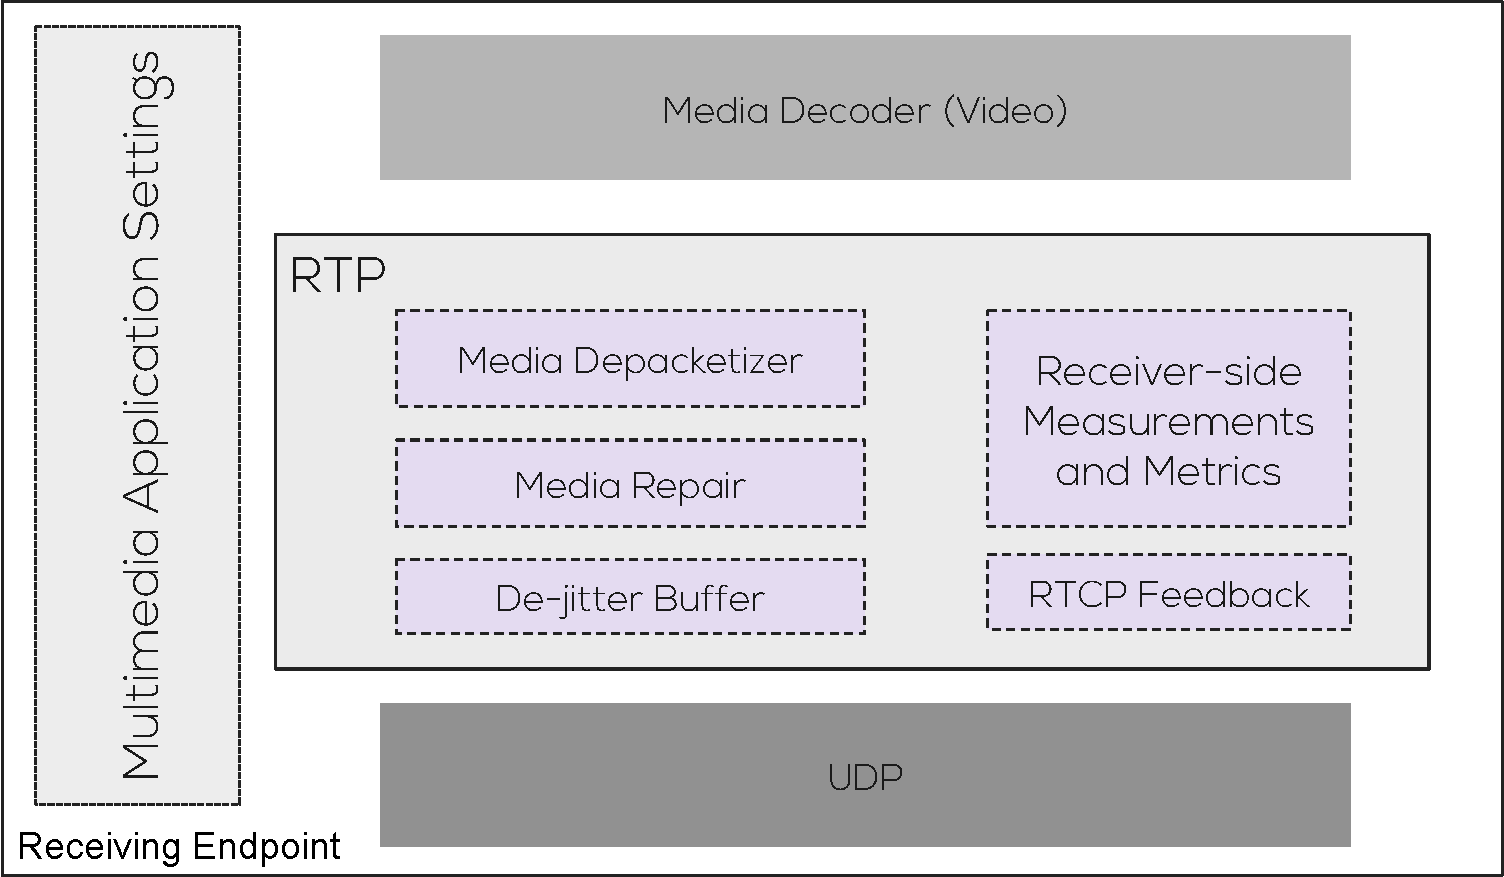
\includegraphics[width=0.66\textwidth]
      {chap4_fig_app_receiver}
    }
  }
  
  \caption{Typical architecture of a multimedia system. a) sending endpoint,
  b) receiving endpoint.}
  \label{fig:4:appint}
\end{figure}

Figure~\ref{fig:4:appint} shows a simplified architecture of a sending and
receiving endpoint; typically, a real-time multimedia application would
contain both these systems and perhaps even two of each for handling audio and
video separately. Figure~\ref{fig:4:appint} (a) depicts the features of the
sending-side RTP stack. The \emph{media packetizer} subsystem receives a video frame or a
series of audio frames from the codec, which it packetizes into RTP.  The
resulting RTP packets are then passed on to the \emph{media redundancy} subsystem to
be cached if a NACK is received or for producing FEC packets. Additionally,
the RTP packet size and count is sent to the RTCP subsystem for creating RTCP
SR packets. Simultaneously while passing the packet to the media redundancy
subsystem, the RTP packets are sent to the \emph{pacing buffer or scheduler} subsystem which
transmits the packets in a single burst or trickles them on to the network
before the next set of RTP packets are generated by the media packetizer or codec. The
sending endpoint also routinely generates and receives RTCP packets. 
The RTCP RR packets are sent to the \emph{RTCP feedback} subsystem and 
onwards to the \emph{Rate Controller} subsystem.
The rate controller monitors the congestion cues and based on the congestion control
algorithm calculates the  new target encoding rate. The codec attempts to
compress the media stream to meet the new target encoding rate in a reasonable
time frame. Figure~\ref{fig:4:appint} (b) depicts the features of the
receiving-side RTP stack. The received RTP packet is put in a \emph{dejitter buffer}
to reassemble out-of-order packets. The dejitter buffer may discard late
arriving packets and it also detects packet loss. Furthermore, the packet
sequence number, size of the packet, RTP timestamp and the reception
timestamp are passed to the \emph{RTCP feedback} subsystem, which routinely generates an
RTCP RR packet and may additionally generate requests for retransmitting
missing RTP packets. This information is also shared with \emph{receiver-side
measurements and metrics} subsystem, which may generate additional congestion
cues to be sent along with the RTCP RR as RTCP extended reports (XRs). If FEC
packets or other types of repair packets are received, they are passed on to
the \emph{media repair} subsystem which attempts to recover the missing packets in
the dejitter buffer. The dejitter buffer size is typically configured to a small value to maintain
communication interactivity, so packets are sent to the \emph{media packetizer} where
an audio or video frame is reconstructed and sent to the decoder for playback.


We identify three control loops to implement congestion
control~\cite{Singh:control.loops.api} based on the interaction between the
above components in an multimedia system~\cite{draft.rmcat.app.interaction},

\begin{enumerate}
\setlength{\itemsep}{0pt}

\item \textbf{\texttt{Codec-Sender}}: The codec adapts its encoding rate based
on the feedback from the sender. Unlike elastic traffic, the codec is unable
to produce the expected media rate immediately. Therefore, the rate-controller
needs to take into account the timeline in which the codec produces the new
rate.

\item \textbf{\texttt{Sender-Network}}: The sender packetizes media frames and
sends them over the network to the receiver. The sender may however pace the
fragmented frames on to the network instead of sending them in a single
burst. It also collects feedback messages from the receiver that may contain
congestion cues (i.e., variation in RTT, indication of lost or discarded
packets, goodput, jitter, etc.).

\item \textbf{\texttt{Receiver-Sender}}: The receiver has a playout buffer of
media data waiting to be decoded and rendered, discarding packets that arrive
late for playout, and attempting to conceal the missing packets from the
observer. The receiver also monitors the media flow for packet losses,
variation in jitter, receiver rate, goodput, etc. and reports these to the
sender to act upon.

\end{enumerate}

If an endpoint detects congestion rapidly, and the end-to-end path latency is
sufficiently low so that this information can be communicated quickly, it is
possible to change the encoding rate promptly to meet the variation in the 
end-to-end path capacity. However, in practice, this is not always possible because
\textbf{a)} it may take multiple reports or data packets to detect congestion, and
\textbf{b)} after detecting congestion, it takes at least a one-way delay (OWD)
amount of time for the receiver to report it.


\section{Congestion Cues}
\label{fw.cues}

Congestion control algorithms rely on cues to detect congestion. These cues
are detected either by the sender, receiver, or by an intermediary router. The
endpoint observes the congestion along the path and accordingly adapts the
sending rate upon receiving the congestion cues. 
Some common congestion cues are listed below:

\begin{itemize}
\setlength{\itemsep}{0pt}

\item \textbf{\texttt{Losses}}: occur when intermediate routers drop packets
from their queues (\emph{congestion loss}), or due to contention, interference
or fading on wireless link (\emph {bit-error loss}). Losses are inferred at
the receiving endpoint by gaps in RTP sequence numbers. Typically, a dejitter
buffer is used to reorder out of order packets and the fraction packet loss is
calculated at the end of each reporting interval.

\item \textbf{\texttt{Discards}}: packets that arrive too late at the receiver
to be decoded or played back may be discarded by the receiving endpoint. These
late-arriving packets are discarded by the receiver even though they are
received because packets with higher \textit{timestamps} have already been
passed to the decoder for playback. The fractional loss in the standard RTCP
RR does not identify these discarded packets as lost, hence they need to be
reported in an RTCP XRs.

\item \textbf{\texttt{Sending rate, receiver rate and goodput}}: are measured
at the sender, the receiver and at the decoder, respectively. Typically, the
sending rate is the rate at which the media bit stream is generated by the
encoder. If packets are lost in the network, the receiver rate is lower than
the sending rate. Or if duplicate packets are received, the receiver rate is
higher than the sending rate. Lastly, if packets are discarded after arrival
or dropped by the decoder, the goodput will be lower than both the sending
rate and receiver rate. Hence, goodput represents the actual playback bit rate
or the bit rate of the rendered bit stream.

\item \textbf{\texttt{One-way delay (OWD)}}: is a combination of
\emph{propagation}, \emph{queuing}, \emph{serialization} and \emph{processing}
delay. Propagation delay is calculated from the ratio of the physical length
of the interconnected link and the propagation speed over the specific
medium\footnote{Usually, propagation speed is a fraction of the speed of light
($0.5$c-$0.8$c).}. The serialization delay is the time taken to send a
complete packet on to the communication channel (link) and is a function of
the link rate and the packet size. The processing delay is the time taken for the
router to determine the next hop or the destination of the packet. Lastly,
when multiple packets are received, the router queues them and transmits them
one by one. Having large-sized buffers in the router causes \emph{buffer-bloat}
\cite{gettys:bufferbloat} and increases the overall one-way delay.
However, measuring one-way delay is difficult because the clocks at the
endpoints are normally not synchronized; instead, the endpoints rely on RTT
measurements for congestion control.

%In a multihop environment, these delays are calculated per hop.

\item \textbf{\texttt{Round trip time (RTT)}}: is the time taken for a packet
to go from the sender to the receiver and then back. In RTP, it is calculated
with the collaboration of sending RTCP SRs and receiving RTCP RRs. In
conversational multimedia, the media flows in both directions, so the one-way
delay (OWD) is approximated as half of the measured RTT. Observing the changes
in RTT provides an indication of congestion and smoothing the RTT
(averaging over a short interval) protects against over-reacting to the subtle
changes in RTT.

\item \textbf{\texttt{Packet delay variation and packet inter-arrival time}}:
packets may arrive at different times due to route changes, or congestion at
the bottleneck link causes jitter. Endpoints detect jitter by comparing the
send or media generation timestamps with the receiving timestamps. The
variation in inter-arrival time may be used to infer congestion.

%\item \textbf{\texttt{Adaptive playout time or Size of Receiver buffer}}:

\end{itemize}

To pick the right congestion cue, an algorithm developer should consider the
following: the type of media stream (audio or video), the expected packet or
frame rate, typical MTU size, interdependence of the streams (audio/video
sync, multi-view video), whether the congestion controller knows the operating environment (Internet-scale, 
low-delay local area deployment, heterogeneous environment with a mix
of wired and wireless links) and the application requirements (audio preferred
over video or vice versa).

Another aspect to consider when picking congestion cues is the the monitoring
duration to identify congestion, i.e., either over a \emph{long-term} (order
of seconds or minutes) or a \emph{short-term} (order of 100\,\emph{ms} or a
few seconds). For example, jitter is measured on a per-packet basis, but
reported over a longer measurement interval (to filter for noise and
transience). In contrast, packet losses, discards, etc. are measured over a
shorter interval so that the sender can react to these immediately.

\section{Congestion Reporting Frequency}
\label{fw.freq}

Normally, congestion control requires a tight control loop, which means that
the receiving endpoint should be able to provide feedback at very short
intervals (at least once per RTT). Hence, the design of a congestion control
algorithm needs to be aware of the limits on the timing of the feedback. For
example, in TCP, the receiver sends an \emph{acknowledgment} packet in
response to every packet (or every few packets) it receives, whereas RTCP
encourages infrequent feedback and specifies an upper-bound on the fraction of
the session media bit rate that the feedback packets can use\footnote{The
specified feedback rate is 5\,\% for each multimedia session.}.
\cite{draft.rmcat.feedback} discusses three options for the short report
intervals,

\textbf{\texttt{Per-packet feedback report}}: sends RTCP feedback every time
the endpoint receives a packet. For low bit rate media sessions (e.g., audio
streams), this would be quite difficult to achieve because the size of the
feedback packet would be comparable to the size of the media packet, i.e., the
feedback bit rate would larger than the 5\,\% fraction specified for it. If an
endpoint receives packets in a burst or at very short time intervals, the
endpoints will not be able to meet the timing requirements for per-packet
feedback because the RTCP timing interval calculation has a randomization
factor to avoid synchronizing feedback from multiple endpoints.

\textbf{\texttt{Per-frame feedback report}}: sends RTCP feedback every time
the endpoint receives a complete frame. This is mainly applicable to video
where a single video frame would be fragmented into multiple packets because
the frame size exceeds MTU size. Typically, an average size of an RTCP packet
size in a two-party call is $156$-$176$ bytes\footnote{The packet breakdown in
bytes is: UDP=16, IPv4=20 or IPv6=40, RTCP=8, SR=20, RR=24, SDES=28, one or
more XR blocks is 20 bytes each.}. For a 30 FPS bidirectional video stream, the
$rtcp\_bw \approx$ 75\,\emph{Kbps}, which requires the media session bit rate
be set to a value higher than 1.5\,\emph{Mbps}. Consequently, it would not be
possible to perform per-frame for sessions with lower media rates. It should
be noted that the requirements for the media session bit rate needs to be 
re-calculated if the number of participants change, the number of reported
blocks change, or the frame rate changes.

\textbf{\texttt{Per-RTT feedback report}}: sends RTCP feedback at regular
intervals based on the RTT estimate. The requirement for the media session
rate would be lower, if the RTT is higher than the frame inter-arrival time.
The calculation of the RTCP interval for the per-frame still applies, except
that the frame rate is replaced by the RTT estimate.

To summarize, picking longer RTCP feedback intervals requires a lower media
session bit rate, hence it increases the possibility of applying the same
congestion control to a larger operating area (in terms of session media
rates).

\section{Framework for Classifying Congestion Control}
\label{fw.fw}

A rate-control or congestion control algorithm relies on congestion cues to
pick a new sending rate. These cues are either observed at the receiver or by
intermediaries monitoring the flow, or are aggregated by a
third-party\footnote{A system outside the signaling or media path} or a
super-peer in an overlay network. Consequently, these observed cues need to be
signaled back to the sender which will perform congestion control. We classify
these congestion cues as a combination of \emph{where are they
measured/observed?}, and \emph{how is the sender notified?} For each, there are
two options: In-path and Off-path \emph{sources} and In-band and Out-of-band 
\emph{signaling}~\cite{Singh:PhDFw}. In-path congestion cues are measured
by the receiver or by intermediaries along the path. Off-path congestion
cues are reported by devices outside the media path (congestion maps,
overlays, etc.). The combination forms four cases which are visualized in
Figure~\ref{fig:4:fw}.

\begin{figure}
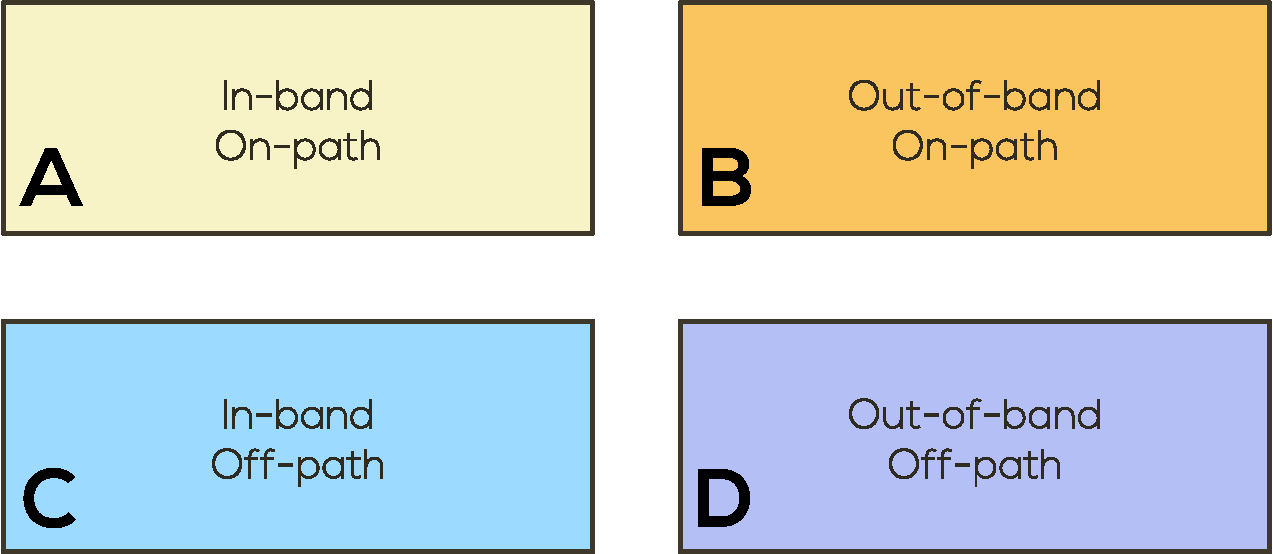
\includegraphics[width=0.9\textwidth]{chap4-fig-fw-outline}
\caption{Framework for classifying congestion control~\cite{Singh:PhDFw}.}
\label{fig:4:fw}
\end{figure}

A congestion control algorithm needs to pick one or more measurement point
(picking multiple adds to the feedback overhead) and then choose a method
to signal it to the sending endpoint. The algorithm can choose to report it in-band by
encapsulating the cues, either by piggybacking them on the endpoint's own media
packets as RTP header extensions (this adds to the header overhead of a media
packet) or as RTCP extension blocks (see section~\ref{fw.freq} for details on
feedback frequency). Or the congestion control algorithm can choose to signal
the cues out-of-band, i.e., re-use the signaling path (e.g., SIP, XMPP) or
setup an alternate signaling path (e.g., HTTP or websockets). THe following are
examples for each category in the framework:

\textbf{\texttt{A) In-path, In-band}}: The congestion control algorithm in
this case relies on the cues reported in an RTCP feedback from the receiver.
For example, TFRC using information in RTCP RR, TFRC using additional loss
reported by ECN markings, Temporary Maximum Media Stream Bit Rate Request
(TMMBR), Receiver Estimated Max Bit rate (REMB).

\textbf{\texttt{B) In-path, Out-of-band}}: The congestion control algorithm
relies on the cues reported in the signaling channel; for example, RTSP implements
a \emph{Speed} parameter to vary the transmission rate, or 3G base stations announce
the new rate when capacity changes due to cell-loading or handover.

% announcing bandwidth in the SDP at the start of the session (instead of
% starting at a low media bit rate) for rudimentary congestion control,

\textbf{\texttt{C) Off-path, In-band}}: The congestion control algorithm
relies on reports from multiple in-band sources; for example, in Multipath
RTP, congestion on one path causes a change in the fractional distribution of
traffic on each path.

\textbf{\texttt{D) Off-path, Out-of-band}}: The congestion control
algorithm relies on third party sources such as receiving bandwidth or
congestion notifications from congestion maps, bandwidth lookup services,
super-peers and overlays.

% monitoring: long-term, short-term

% Additionally if the cue reliably
% describes the onset of congestion (\emph{knee}) or the collapse
% (\emph{cliff}).

% \begin{figure}[!h]
% 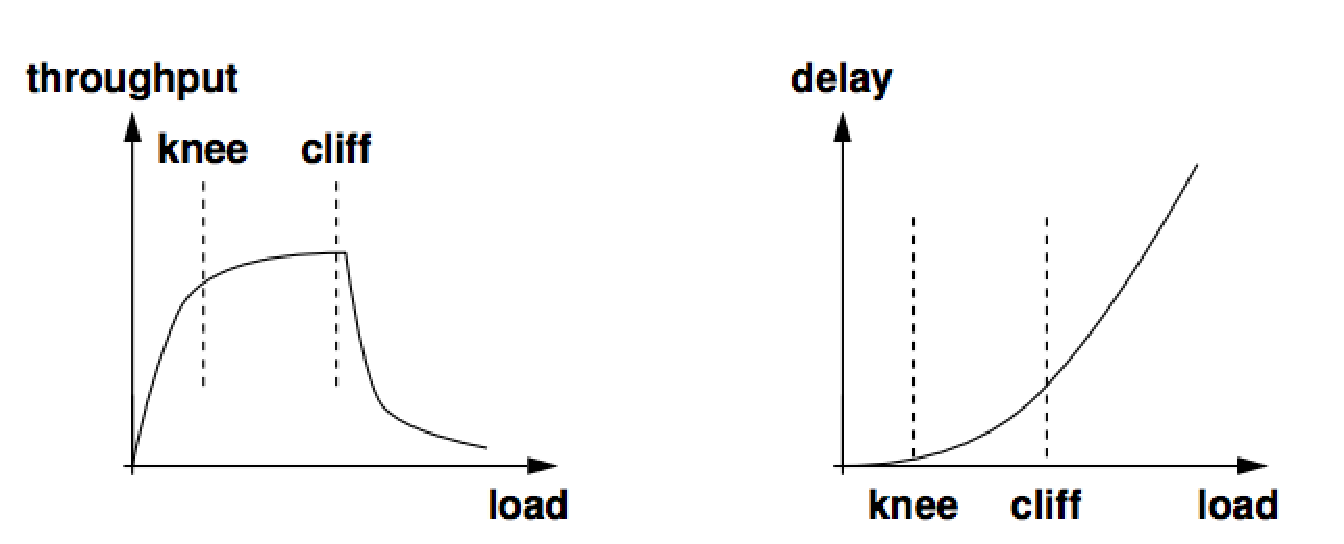
\includegraphics[width=\columnwidth]{chap4-knee-cliff}
% \caption{Shows the variation throughput and delay with increasing network load.}
% \label{fig:4:knee}
% \end{figure}

\section{Congestion Control Evaluation}
\label{fw.cc.eval}

% We need to define a set of requirements in order to design a congestion
% control algorithm for multimedia streams. Later these requirements are used as
% a checklist to evaluate the suitability of the proposed algorithms.

Real-time interactive communication differs greatly from \emph{elastic}
traffic because the sender generates media packets in real-time and expects it
to be delivered in hundreds of milliseconds, and the receiver consumes the media
packets almost immediately, hence late-arriving packets are useless.
Additionally, real-time communication systems are able to tolerate some amount
of packet loss and adapt the media rate over a fairly large range.
\cite{draft.rmcat.req} lists a set of requirements for RTP-based interactive
multimedia sessions; these requirements form the basis of the guidelines
described in~\cite{draft.rmcat.evaluate}. In~\cite{draft.rmcat.eval.test}, we
define a catalog of \emph{traffic flows} traversing through a \emph{network
topology} with varying \emph{link characteristics} and diverse \emph{queuing}
strategies. By picking one feature from each category, we
construct scenarios to evaluate the performance of the congestion control. The
evaluation scenarios are built using the following components: network
topology, link and router characteristics.

The difference between testing in real-world deployments and in simulations is
also important to consider, mainly in terms of the accuracy of RTT
measurements which impacts delay-based algorithms (e.g., TFRC). Time-slot-driven
simulation systems, such as \emph{ns-2}~\cite{ns2}, have accurate timing that
is not representative of real-world systems. Testbeds usually use
dummynet~\cite{Carbone:2010p3502}, NetEm~\cite{netem}, or packet traces to
emulate the variation in link capacity, latency, intermediate router queue
length, and packet losses. 

It is also possible to use actual machines placed at geographically distinct
locations and send media traffic between them; however, in this case, it is
not possible to run a controlled experiment anymore because of the varying
amount of cross-traffic generated by other hosts in the network.  Usually the
last step in the evaluation process involves deploying the congestion control
algorithm on several (thousands of) endpoints and showing that it behaves as
described without breaking anything on the network (i.e., causing a congestion
collapse).

\subsection{Network flows}

In this section, we describe typical test scenarios for evaluating congestion
control algorithms. These test scenarios are not supposed to be exhaustive
but show the applicability range of the algorithm.

\begin{enumerate}
\setlength{\itemsep}{0pt}

\item \textbf{\texttt{Single media flow on an end-to-end path}}: This scenario
describes the best case, wherein the network puts each flow identified by its
5-tuple (protocol, source and destination IP address, source and destination
port numbers) in its own queue, thus the flow using the proposed congestion
control algorithm does not encounter any cross-traffic.

\item \textbf{\texttt{Single media flow competing with multiple similar
flows}}: In this scenario, the flow using the proposed congestion control
algorithm competes with multiple flows using the same congestion control algorithm
(i.e., all flows are interactive multimedia).


\item \textbf{\texttt{Single media flow competing with multiple TCP flows }}:
In this scenario, the flow using the proposed congestion control algorithm
competes with TCP flows. These maybe \emph{short} TCP flows representing
common web-traffic patterns or \emph{long} TCP flows depicting bulk transfers
(e.g., large file downloads).

\end{enumerate}

% In Section~\ref{rg.title}, we describe the network traffic scenarios to
% evaluate the proposed congestion control algorithms, namely, when the flows
% are a) alone, b) competing with self-similar flows, and c) competing with TCP
% flows (short-, long-lived) on a bottleneck link.




\subsection{Link characteristics}

The link characteristics can be broken down into the following categories:
capacity, latency, and loss. The capacity of a link mainly varies in wireless
networks (for example in 3G, LTE, WLAN, etc). In Wireless LAN (WLAN) networks,
the capacity varies depending on the density of nodes using the network. The capacity in
mobile networks (e.g., 3G, LTE) fluctuates for each user because of fading,
interference, mobility, handover, cell loading, etc. The latency of a link
is measured as the propagation and serialization delay. Queuing delay is based on the
queue size of the router and hence, is a router characteristic. Latencies between
nodes typically vary from a few milliseconds to a few seconds. Commonly used
values are: LAN (very low delay, <1\,\emph{ms} ), low delay (<40\,\emph{ms}),
trans-continental (>100\,\emph{ms}), or satellite links (>500\,\emph{ms}).
Packet losses are modeled using the Gilbert-Elliott
Model~\cite{gilbert1960capacity, elliott1963estimates} or by packet
traces~\cite{ellis:2011:dataset, 3gppSim}.


\subsection{Router characteristics}

 % Queue-size and Queue type.

Apart from managing packet routing, a router also manages congestion; when a
packet arrives at a higher rate than it can be processed, the router queues the
packet. The routers then use \emph{priority queuing}, \emph{fair queuing}, or
\emph{weighted fair queuing (WFQ)}~\cite{rfc4594} to decide which traffic
class to transmit or drop packets from during congestion. When congestion
occurs within the same traffic class, the router discards packets using
\emph{tail drop}, \emph{Random Early Detection (RED)}~\cite{Floyd:RED}, or
\emph{Weighted Random Early Detection (WRED)}.

We describe the queue sizes as a function of time, i.e., it is the depth of
the queue or the amount of time the packet will remain in the queue before it
is discarded. However, in practice, the queue size is measured in number of
packets. We convert the queue depth (measured in time) to queue length (number
of packets, MTU is typically 1500 bytes) using:

\begin{equation*}
  \mathrm{QueueSize}_\mathrm{packets} = 
    \frac{\mathrm{QueueSize}_\mathrm{sec} \times
    \mathrm{Throughput}_\mathrm{bps}}{\mathrm{MTU} \times \mathrm{8}}
\end{equation*}

For example, a router with a throughput of 1\,\emph{Mbps} and a 1\,\emph{s} queue depth would be
capable of handling 83 packets (queue length). A 100\,\emph{ms}
queue depth may represent a short queue, while a 10\,\emph{s} queue depth represents
a buffer-bloated queue.

\subsection{Network topology}

We should run different types of network topologies to evaluate the
performance of congestion control. Depending on the amount of cross-traffic,
the bottleneck link will move from one node to another in the network. Also,
the bottleneck in each direction may be different due to the asymmetry of
access links. Additionally, the varying capacity of the access link (e.g., in
wireless environments) may be the bottleneck.


\begin{figure}
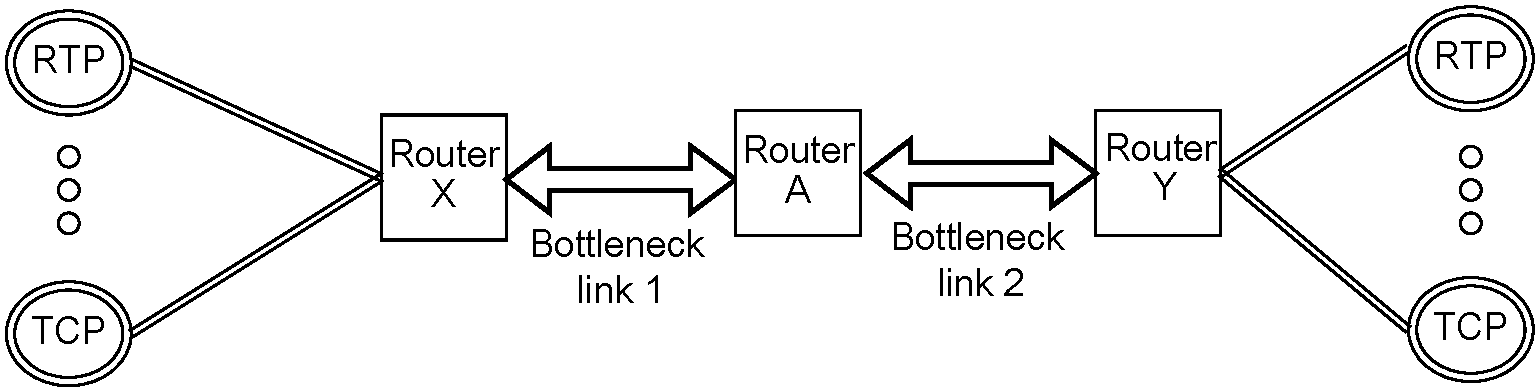
\includegraphics[width=\textwidth]{chap4_fig_sim_topology}
\caption{Typical network topology for evaluating congestion control consisting
of traffic flows (evaluating flow and cross traffic), links and routers.}
\label{fig:4:topology}
\end{figure}


Figure~\ref{fig:4:topology} shows an example of the evaluation setup. This
topology is commonly called the \emph{dumb-bell} topology. Another common
topology is \emph{parking lot}, which uses multiple bottlenecks instead of a
single bottleneck; however, both use common concepts.


To define a scenario, we need to choose the following: the type of cross-
traffic (self-similar, short- or long-lived TCP), the characteristics of the
cross traffic (e.g., duration), the characteristics of the edge routers
(Router X and Y) and the impairments in the network. Lastly, we have to
measure and analyze the performance of the multimedia system.


\subsection{Our Evaluation Setup}

Our research made use of the network simulator (\emph{ns-2})~\cite{ns2} or a
testbed made up of real-machines. The individual link characteristics in the
testbed were either controlled by NetEm~\cite{netem} or by
dummynet~\cite{Carbone:2010p3502}; the intermediate machines that ran
NetEm/Dummuynet ran kernels re-compiled at 1000Hz for better performance. The
endpoints typically ran stock Linux, such as Ubuntu 10.04 or 12.04. In some
cases, we used bandwidth and packet loss traces provided by
3GPP~\cite{s4.eval.bitrate} or collected them ourselves~\cite{sharmistha-thesis}. 
Additionally, we ran some tests between machines in Helsinki and the
Amazon data centers located in Virgina (US-EAST) and Ireland. The details of the
individual test scenarios are discussed in detail in the associated scientific 
papers.

\subsection{Metrics for Çongestion Control}
\label{subsec.metrics}

In this section, we introduce metrics for evaluating congestion control
algorithms. Multimedia application observe the congestion cues, and react to
the changes in the cues, by modifying the encoding/sending rate to match the
available end-to-end bit rate. The sender's goal is to minimize losses at the
receiver while maintaining a stable throughput. Losses are caused by
congestion or by  bit-errors and are detrimental to video quality. Although,
real-time communication is tolerant to a small amount of losses, bursty loss
should be avoided.  

% Bit-errors are due to the physical properties of the network and cannot be
% predicted ahead of time. Congestion losses are due to over-utilization of the
% links and may cause long delays or congestion-induced drops at the router.



\begin{figure}
\centering
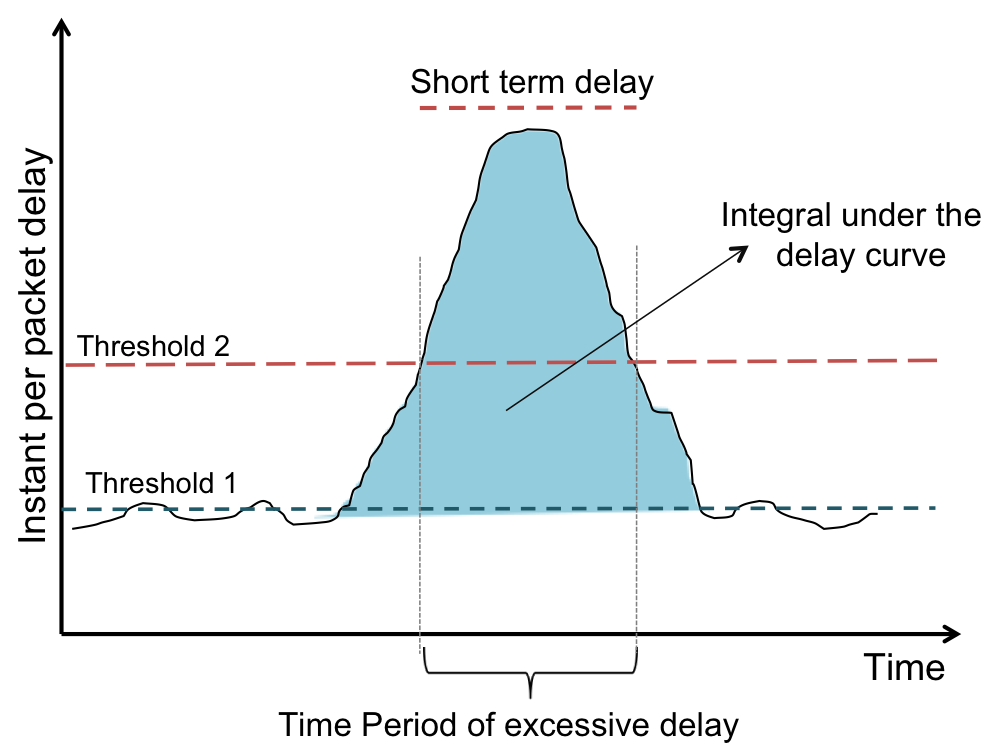
\includegraphics[width=0.75\textwidth]{chap4_fig-perf-metrics}
\caption{Metrics for congestion control.}
\label{fig:4:rc_model}
\end{figure}

Figure~\ref{fig:4:rc_model} schematically shows the instant per-packet delay
over time observed at the receiver. The sender reacts to the changes in the
available path bit rate. Exceeding the available path bit rate may lead to a
temporary increase in per-packet delay until the rate adaptation measures take
effect and, optionally, to packet losses if the queue capacity is exceeded.

For the delay, we define three values:
\begin{itemize}
\setlength{\itemsep}{0pt}

\item \textbf{\texttt{Threshold 1}} refers to the mean one-way delay observed
under normal operating conditions; this value may be defined statically
according to expectations for a certain environment, or determined
dynamically. This reflects the mouth-to-ear or camera-to-eye delay.

\item \textbf{\texttt{Threshold 2}} defines the maximum acceptable one-way
delay for a packet after which the rendering of the received media packet is
no longer meaningful. Packets arriving later than threshold 2 will be
discarded.

% Threshold 2 may be, e.g., 100-500ms for video, since the human eye
% is more tolerant to video glitches~\cite{s4.eval.fw}.

\item The \textbf{\texttt{short-term delay peak}} reflects the maximum delay
peak encountered during a congestion control operation. This may be either
caused by the appearance of cross-traffic on the bottleneck link or due to
congestion resulting in self-inflicted delay.

\end{itemize}

For losses, we consider two values:
\begin{itemize}
\setlength{\itemsep}{0pt}

\item \textbf{\texttt{Packets lost}} in the network due to bit errors and/or
increased queue lengths or overflows (e.g., caused by drop-tail or RED queue
management).

\item \textbf{\texttt{Packets discarded}} at the receiver because their
arrival delay violated threshold 2.

\end{itemize}

Additionally, we measure the instantaneous and average encoder rate, receiver
rate and goodput. The instantaneous rate is calculated at 1 second intervals. The
Average Bandwidth Utilization (ABU) is the ratio between the instantaneous
goodput (or encoding, receiving bit rate) and the instantaneous channel
capacity at 1 second intervals. An ABU larger than 100\,\% represents over-utilization 
and the duration over which it is over 100\,\% signifies the congestion period.


Peak Signal-to-Noise Ratio (PSNR) is the ratio between the maximum possible
power of a signal and the power of a noisy signal. The maximum power signal is
presumed to be the original signal, while the noisy signal is the received data
signal that has undergone the cycle of compression-transmission-decompression.
While PSNR is the most widely used objective video quality metric, it does not
perfectly correlate with perceived visual quality due to the non-linear
behavior of the human visual system~\cite{itu-t-j247}. Another criticism
against PSNR is that it does not incorporate time in its calculation. Despite
its shortcomings, we use PSNR as a yet another indicator for measuring the
performance of congestion control.

% It has been observed that the pictorial quality perceived by the human visual
% system is also affected by the overall general impression of the viewed video
% stream. In addition, recent studies have shown that human visual system awards
% higher response to more salient image locations and
% features~\cite{Li02asaliency, Ong:2006p3066}.


\section{Circuit Breakers for Unicast RTP Sessions}

If congestion control is not implemented by multimedia applications, they can
cause severe congestion in the network, especially if high data rate media
traffic is sent over low-capacity networks. This can not just disrupt the
multimedia's quality of experience but also other applications on the network.

We are developing a circuit breaker algorithm that can work with unmodified
RTP applications to determine when these non-adaptive multimedia
applications are causing excessive network congestion and force them to cease
transmission.  We envision that the congestion control algorithms for
multimedia standardized in the IETF will need to work inside the envelope of
this circuit breaker algorithm~\cite{draft.rmcat.evaluate}, i.e., a multimedia
application implementing congestion control should not trigger the circuit
breaker. Consequently, the circuit breakers cannot be too aggressive in
terminating media flows because it should allow sufficient time for the
congestion control algorithm to monitor and respond to congestion cues.

The circuit breaker algorithm in the short term will serve as a policer,
during which time the congestion control algorithm is developed. Developing
standard congestion control algorithms for unicast RTP-based interactive
multimedia applications is expected to be a multi-year process in the IETF.
Therefore, the development of the circuit breaker is on a tight schedule, to
be ready for inclusion in the initial roll-out of the WebRTC (Web-based 
Real-time Communication) framework~\cite{jennings:2013:webrtc} in web browsers.

\subsection{Circuit Breaker Design}
\label{fw.cb.design}

The RTP circuit breaker algorithm relies on the basic feedback mechanisms
defined in the RTP Control Protocol (RTCP)~\cite{rfc3550}. That is, it solely
uses the information available in the RTCP Sender Report (SR) and Receiver
Report (RR) packets to detect if the flow is overusing the capacity or causing
congestion.

The congestion indicators considered for implementing circuit breakers are: 1)
the network \emph{round trip time} (RTT) calculated  using timing information
in RTCP SR and RR packets, 2) the \emph{jitter} estimated by the receiver over the
last reporting interval, and 3) \emph{fractional packet loss} and \emph{cumulative
loss} reported by the receiver during the last RTCP interval. These
indicators  unfortunately only provide a limited insight into the behavior of
the network and cannot be used as strong signals for a circuit breaker.

Variation in RTT is used as a congestion indicator in delay-based congestion
control algorithms. Additionally, some algorithms use RTT estimates to
configure connection timeouts. In RTP/RTCP, the RTT is estimated infrequently
because the feedback intervals are rather long, making it difficult to detect
the cause in variation of delay. Likewise, variation in jitter can indicate a
transient network congestion but does not provide a strong enough signal to implement
a circuit breaker. On the other hand, loss is a strong indicator of congestion
in networks where packet losses predominantly occur due to queue overflows, and
is a less accurate indicator where packet loss occurs due to bit-error
corruption (e.g., wireless and mobile links). Therefore, we base the circuit
breaker conditions on packet losses. 

\begin{enumerate}
\setlength{\itemsep}{0pt}

\item \textbf{\texttt{Media Timeout}}: An endpoint is sending media data but when
the receiver reports a non-increasing \emph{Highest Sequence Number} (HSN) for
two consecutive RTCP intervals, the flow is terminated.

\item \textbf{\texttt{RTCP Timeout}}: An endpoint is sending media data but if it
receives no RTCP RR for three consecutive RTCP intervals, the flow is
terminated.

\item \textbf{\texttt{Congestion}}: An endpoint is sending media data and if it
receives RTCP RRs indicating fractional packet loss, it calculates the TCP-friendly 
rate and compares it to the sending rate. If the sending rate exceeds
the TCP-friendly rate  by a factor of 10 for two consecutive RTCP intervals,
the flow is terminated.

\end{enumerate}

Full details of the RTP circuit breaker algorithm is specified
in~\cite{draft.rtp.cb}, which is a work in progress and covers various
deployment cases such as multiple media sources, impact of shorter-than-standard 
reporting interval, deployment of Explicit Congestion Notification
(ECN), etc.

In \citepub{c:cb}, we apply these circuit breaker conditions to non-adaptive
RTP media flows deployed on ADSL and cable modem links.  Such flows typically
do not implement congestion control at this time, and are likely to cause
congestion if deployed on the Internet. We carried out a series of experiments
based on real-world traces and on a testbed emulating real-world conditions.
Our results show that the proposed RTP circuit breaker performs well,
triggering in cases of bursty loss and in sessions that are congesting the
links, and does not trigger in low-loss and non-bursty scenarios.


\begin{figure}
  \centering{
    \subfloat[Non-bursty]{
      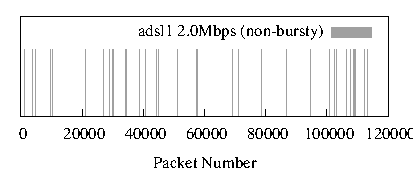
\includegraphics[width=0.66\textwidth]
      {chap4_graph_cb_20090707-1515-barcode}
    } \\
    \subfloat[Bursty]{
      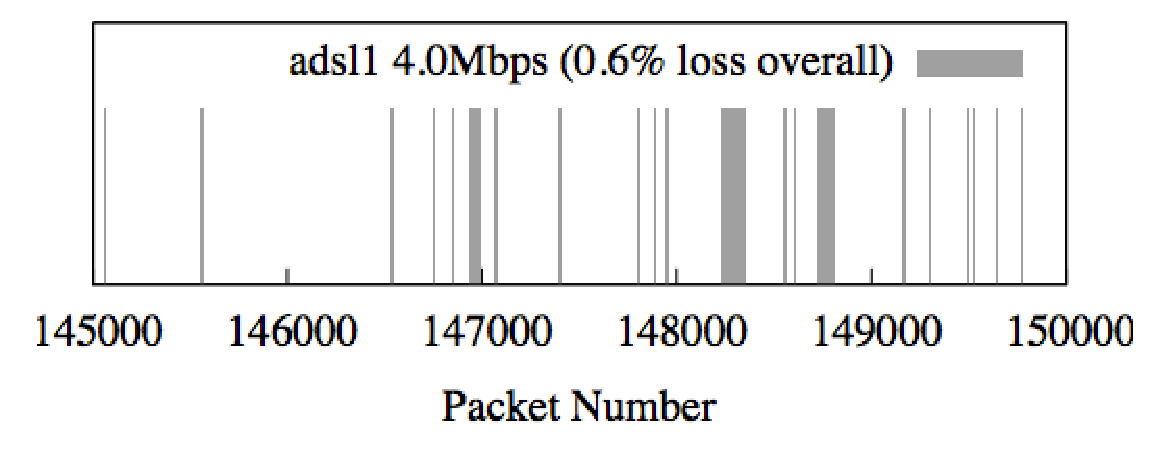
\includegraphics[width=0.66\textwidth]
      {chap4_graph_cb_bursty}
    }
  }
  \caption{Sample non-bursty (a) and bursty (b) packet loss traces.
  The bursty packet triggers the circuit breaker even though the overall
  packet loss ratio is 0.6\,\%.}
  \label{fig:4:bursty}
\end{figure}

\begin{table}
  \begin{center}
    \begin{tabular}{rcc}
    \toprule
      \textbf{Loss Pattern}   & \textbf{Triggered} & \textbf{Did not trigger} \\
    \midrule
             Loss free &   0.0\,\% & 100.0\,\% \\
       Non-bursty loss &   0.0\,\% & 100.0\,\% \\
          Bursty loss  &  11.9\,\% &  88.1\,\% \\
    \bottomrule
    \end{tabular}
    \caption{Sessions triggering the circuit breaker by loss pattern.}
    \label{tab:4:cb_bursty}
  \end{center}
\end{table}

We simulated the RTP circuit breaker performance on $3833$ generated RTCP traces
corresponding to the measurements collected in \emph{dataset-A} and
\emph{dataset-B} of~\cite{ellis:2011:dataset}. Of these, $1626$ traces have no
packet loss, and hence cannot trigger the RTP circuit breaker. The remaining
traces each include at least one lost packet. We categorize the remaining
traces into two categories: those that have non-bursty packet loss, and those
that exhibit bursty loss using the definition of bursty loss
from~\cite{rfc3611} (Figure~\ref{fig:4:bursty} shows representative samples of
the non-bursty and bursty packet loss patterns). The data comprises $1344$
traces with bursty loss and $863$ traces with non-bursty loss.



Table~\ref{tab:4:cb_bursty} shows the fraction of sessions that triggered the
RTP circuit breaker for each of the categories of packet loss. The RTP circuit
breaker did not trigger for sessions without loss; it also did not trigger for
any of the sessions with non-bursty packet loss. However, we observe that the
RTP circuit breaker is triggered more often in sessions that contain bursty
packet loss. 

\begin{figure}[!t]
  \centerline{
    {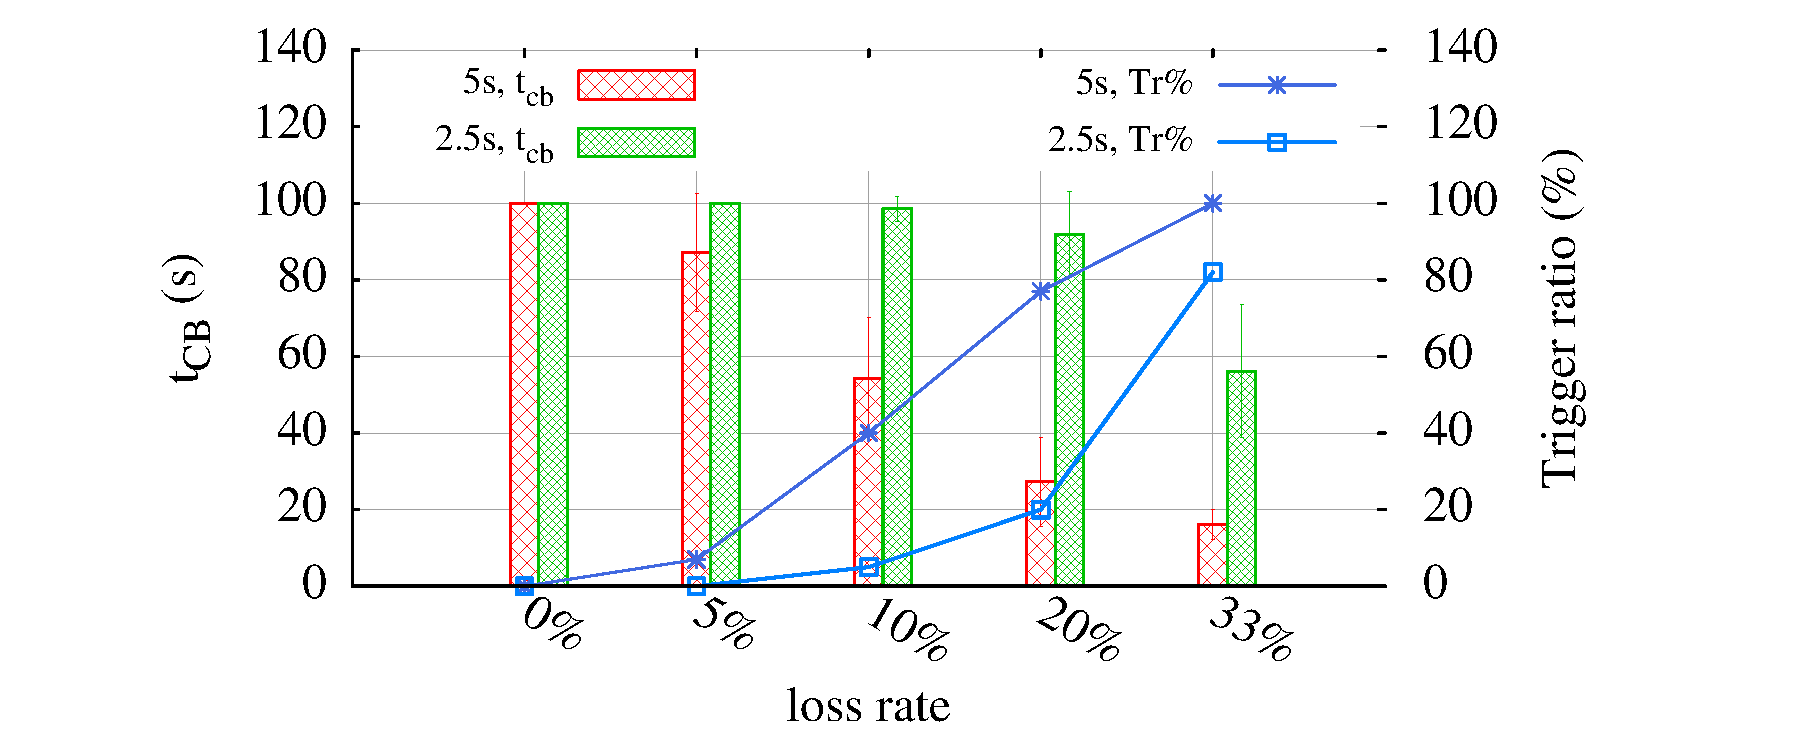
\includegraphics[width=\textwidth]{chap4_graph_cb_cmp_trr_2s}}
  }
  \caption{Impact of using a shorter RTCP interval on the
  circuit breaker. Each scenario was run 50 times and the error bars represent
  the 95\,\% confidence level.}
  \label{fig:4:short-rtcp}
\end{figure}

The circuit breaker conditions trigger mainly due to loss. Figure~\ref{fig:4:short-rtcp} 
shows that the percentage of sessions triggering the circuit breaker
increases with the increase in loss rate. The figure also shows the impact of
the RTCP reporting interval, i.e., by reducing the RTCP interval from 5\,\emph{s} to
2.5\,\emph{s}, fewer sessions are terminated. The endpoints become robust to loss of
feedback packets by sending feedback often and we observe a longer time for
triggering the circuit breaker ($t_{CB}$).

\subsection{Discussion about TCP throughput equations}

In Section~\ref{fw.cb.design}, we described the circuit breaker triggers when
the sending rate exceeds the estimated TCP throughput by a factor of 10. We
can estimate the TCP throughput either using Padhye's full TCP throughput
equation~\cite{padhye1998modeling} or using Mathis's simplified TCP throughput
equation~\cite{mathis1997macroscopic}.

In~\cite{padhye1998modeling}, Padhye \emph{et al.} show that the TCP
throughput for a long-lived TCP Reno connection can be estimated using the
following equation:
\begin{align*}
X_{Kbps} = &\frac{8 \times s}{R \times \sqrt{\frac{2*b*p}{3}}+t_{RTO} \times (3 \times \sqrt{\frac{3*b*p}{8}})\times p \times (1+32 \times p^2)}\\
\end{align*}
While Mathis \emph{et al.} in \cite{mathis1997macroscopic} show that under
conditions of low packet loss, Padhye's equation can be simplified to:
\begin{align*}
    X_{Kbps} = & \frac{8 \times s}{R \times \sqrt{\frac{p \times 2}{3})}}
\end{align*}
\begin{itemize}
\setlength{\itemsep}{0pt}
{\footnotesize
\item[] \texttt{X is the transmit rate in Kbps.}
\item[] \texttt{s is the average packet size in bytes.} 
\item[] \texttt{R is the round trip time in seconds. }
\item[] \texttt{p is the loss event rate, $\forall p \in [0.0, \cdots ,1.0]$.}
\item[] \texttt{$t_{RTO}$ is the TCP retransmission timeout value in seconds, usually set to $\mathbf{4 \times R}$.}
\item[] \texttt{b is the number of acknoweldged packets in TCP; typically set $\mathbf{b=1}$.}
}
\end{itemize}
Mathis \emph{et al.} also show that the simplified TCP equation approximates
Padhye's full equation with reasonable accuracy~\cite{mathis1997macroscopic} .


In \citepub{c:cb}, our experiments on residential networks shows that the
simplified TCP throughput equation performs effectively, while using Padhye's
full TCP equation triggers the circuit breaker earlier. The data show that
the full TCP equation tends to be more sensitive to packet loss. In LTE
networks with a combination of a low RTT and high packet loss rate (due to
AQM), the circuit breaker using the simplified TCP throughput equation
does not trigger at all~\cite{Sarker:CB.lte}. However, using the Padhye's full TCP
throughput equation in these cases gives better
performance~\cite{Sarker:CB.lte}. We believe some of this over-sensitivity is
due to averaging packet loss events over long RTCP reporting intervals and the
fact that the RTT is estimated only once in that interval.

Overall, our preliminary results derived from experiments in a testbed,
and simulations based on real-world traces show that
the proposed RTP circuit breaker performs as intended, triggering in the case
of bursty  packet loss and  not triggering in the low-loss and non-bursty
scenarios. 

% The current analysis is based on measurements done in the UK and
% Finland, while these measurements may be representative of residential links
% in Europe, the infrastructure is likely to differ significantly in other parts
% of the world. Therefore, a wider measurement study of the RTP circuit breakers
% would be desirable.


\section{Summary}

In this chapter, we aimed to classify congestion control cues for real-time
communication based on: \emph{where they are measured?} (by in-path or  off-
path sources) and \emph{how they are reported?} (via in-band or out-of-band
signaling). We also describe other fundamental choices needed to implement
congestion control: congestion cues, reporting frequency and  circuit-breaker
conditions. Additionally, we describe a basic evaluation suite for measuring
the performance of any proposed multimedia congestion control algorithm;
derivatives of these test scenarios are used to discuss the performance of
congestion control in this thesis.

We specified the circuit breaker algorithm and discuss the performance of the
circuit breaker applied to non-adaptive multimedia traffic. Our results show
that it works as intended, i.e., it provides enough time for a congestion
control algorithm to respond to congestion cues before triggering the circuit
breaker. We also show that the endpoint can slightly vary the sensitivity of
the circuit breaker by choosing between the full and simplified TCP throughput
equation. In the forthcoming chapters, we discuss our proposals for congestion
control in various environments, several of which work within the constraints
imposed by the circuit breaker algorithm.




\chapter{Congestion Control for Interactive Multimedia}
\label{chap:cc}
Figure~\ref{fig:4:fw} in Chapter~\ref{chap:cc.fw} shows the structure of the
congestion control framework described in this thesis. The framework
categorizes \emph{in-path} sources and \emph{in-band} signaling for
implementing congestion control (corresponds to \emph{Block A} in
Figure~\ref{fig:4:fw}), which are discussed in this chapter. This chapter is
based on our work on congestion control for interactive multimedia
applications, which is documented in \citepub{c:3grc}, \citepub{c:hetrc},
\citepub{c:eval}, \cite{rfc7097},
\cite{draft.xr.bytes.discarded}, \cite{singh:2010.thesis} and
\cite{Singh:control.loops.api}.

In \citepub{c:3grc}, we propose a new congestion control algorithm for the
mobile (e.g., 3G) environment, to be deployed in the IP Multimedia System
(IMS). The main distinction between mobile (e.g., 3G, LTE) and other wireless
environments (e.g., 802.11x) is that the media streams are transmitted using
the \emph{unacknowledged mode}; the packets corrupted due to bit-errors (e.g.,
wireless interference) are not re-transmitted. Hence, the packets incur low
delay, compared to Wireless LAN where corrupted packets are retransmitted by
the link layer. We propose a sender-driven and a receiver-driven congestion
control, and evaluate the performance of the proposed congestion control
algorithm in a simulated environment (in ns-2) using real-world 3G
traces~\cite{s4.eval.bitrate, 3gppSim}. In \citepub{c:hetrc}, we extend the
approach in \citepub{c:3grc} for deployment on the Internet and show that the
congestion control scheme is deployable there as well. In \cite{rfc7097} and
\cite{draft.xr.bytes.discarded}, we propose RTCP XR block extensions that
indicate the number of bytes discarded and run-length encoding of discarded
packets, respectively. These packets are discarded by the receiver because
they arrived too early or too late to be played out by the receiver. This
information is used as a congestion cue by the sender.

% \cite{Singh:control.loops.api} discusses the application and API requirements
% for interactive multimedia congestion control. It describes the two control
% loops: a) between the receiver and the sender, and b) between the media
% encoder and the sending agent. In the first loop, the receiver notifies the
% sender about the current network characteristics. In the second loop, the
% sending agent requests a new media bit rate, and the encoder tries at best to
% meet it, sometimes under-shooting or over-shooting the requested rate.

Lastly, in \citepub{c:eval} we evaluate the performance of a congestion
control algorithm proposed by Google for WebRTC. We evaluate the performance
in diverse scenarios measuring scalability (\emph{how quickly is the
congestion control able to utilize the available capacity}), self-fairness and
competing against bursty cross-traffic. We evaluate the performance of
web browsers implementing the congestion control algorithm in our testbed that
emulates the diverse scenarios.

\section{Schemes of Congestion Control}

The congestion control algorithm can be implemented at the sender, at the
receiver, or the sender and receiver can operate co-operatively. The
\emph{sender-driven} scheme requires that the receiver measures the current
network condition and signals the observed congestion cues to the sender, which
calculates the sender's estimate and uses it as the new sending rate. In the
\emph{receiver-driven} scheme, the receiver calculates the new sending rate
(receiver's estimate) based on the observed congestion cues, and signals the
new rate to the sender, which, on receiving the new rate, adapts the media bit
rate to the received value. The \emph{co-operative} scheme is an extension to the
\emph{sender-driven} scheme. In this case, the receiver calculates the
receiver's estimated rate and signals it along with the observed congestion
cues; the sender at its end calculates its own estimate based on the
congestion cues and chooses a new sending rate, typically a value in between the
sender's estimate and the receiver's estimate. Figure~\ref{fig:cc:scheme}
shows the interaction of the sender and receiver for each scheme. The figure
merely shows the media flow in one direction; however, it should be noted that
the media in the simulation and the emulated testbed actually flow in both
directions unless explicitly mentioned. This is mainly done for the
convenience of representation and followed throughout the remainder of the
thesis.

\subsection{Sender-driven Congestion Control Schemes}

\begin{figure}[!t]
  \centerline{
    \subfloat[Sender-driven Scheme]{
      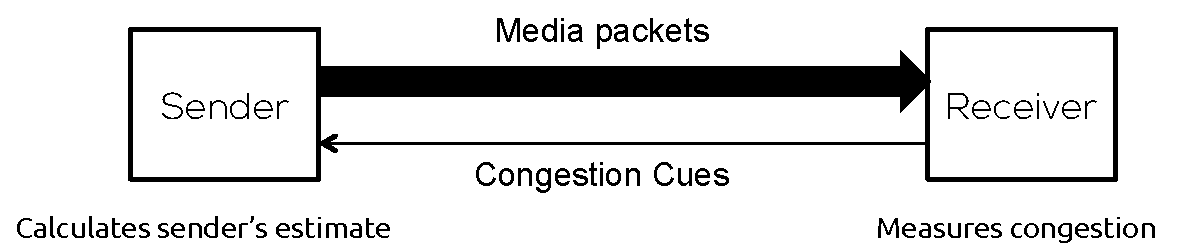
\includegraphics[width=0.9\textwidth]
      {chap5-fig-cc-scheme-s}
    }
  }
  \centerline{
    \subfloat[Receiver-driven Scheme]{
      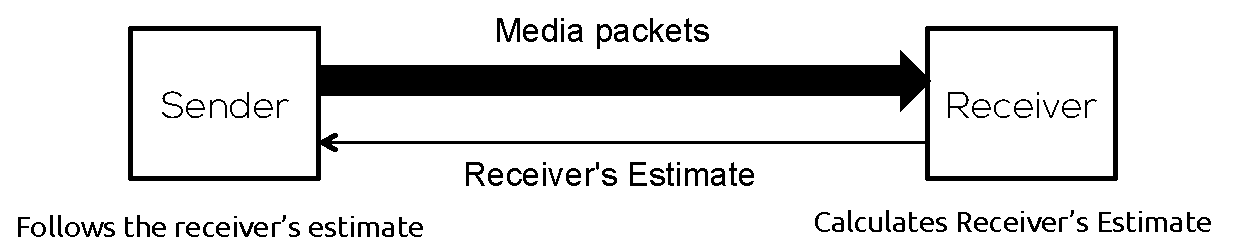
\includegraphics[width=0.9\textwidth]
      {chap5-fig-cc-scheme-r}
    }
  }
  \centerline{
    \subfloat[Co-operative Scheme]{
      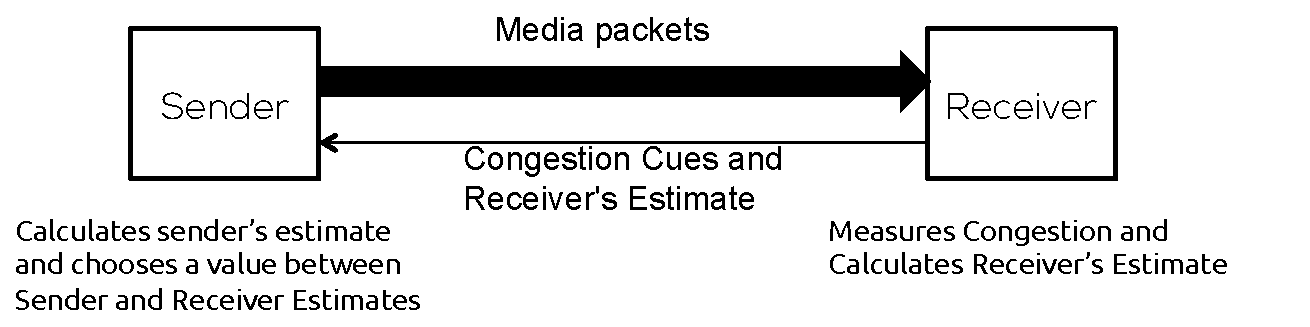
\includegraphics[width=0.9\textwidth]
      {chap5-fig-cc-scheme-c}
    }
  }
  \caption{Congestion control schemes: a) sender-driven, b) receiver-driven
and c) co-operative.}
  \label{fig:cc:scheme}
\end{figure}

TCP Friendly Rate Control (TFRC) is an equation-based congestion control
algorithm implemented at the sender~\cite{tfrc_347397} and is also implemented
as a profile~\cite{rfc4342} in the Datagram Congestion Control Protocol
(DCCP)~\cite{rfc4340}. TFRC uses the average packet size, round trip time
($RTT$), and loss ratio ($p$)~\cite{rfc3448} to calculate the new sending rate.
Formally, the sending rate in TFRC is calculated as follows:

\begin{align*}
 TFRC = &\; \frac{8 \times avg\_packet\_size}
{R \times \sqrt[]{\frac{2 \times b \times p}{3}} + t_{RTO} \times 
\left( 3 \times \sqrt[]{\frac{3 \times b \times p}{8}}\right) \times p \times
\left( 1+32 \times p^2 \right)}\\
where,\; b = &\; 1\\
t_{RTO} = &\; 4 \times R
\end{align*}

TFRC cannot directly be applied to RTP because TFRC requires per-packet
feedback, and in RTP, the RTCP feedback is not necessarily sent that
often~\cite{draft.rmcat.feedback}. Therefore, \cite{draft.rtp.tfrc} maps the
TFRC timing rules defined in~\cite{rfc4828, rfc5348} to that of the RTP/RTCP
feedback loop. It also proposes extensions to the timing rules in the
AVPF-profile~\cite{rfc4585} for very short RTTs ($<20ms$).
\cite{Gharai06:ICME} and \cite{VladBalan:2007dq} show that TFRC is stable on
paths with longer RTTs than those with smaller RTTs, but it too exhibits
saw-tooth behavior~\cite{saurin:2006:thesis}. Any algorithm that consistently
produces a sawtooth media rate is not well suited for real-time communication
because it generates a poor user-experience~\cite{Gharai:2002wt,
Zink03subjectiveimpression}.

Other sender-driven congestion control algorithms that we explored include the
Rate Adaption Protocol (RAP)~\cite{rap:752152} that uses a windowed approach which 
exhibits a sawtooth-type of behaviour. Zhu~\textit{et
al.}~\cite{rmcat-nada} use Pre-Congestion Notification (PCN), Explicit
Congestion Notification (ECN) and loss rate to get an accurate delay
estimate for implementing congestion control. In this case, they assume all
packets marked by ECN and PCN as lost. Their algorithm as specified now, 
relies on accurate measurement of one-way delay relying on clock synchronization.
Instead of just relying on RTT and loss for congestion control, 
Garudadri~\textit{et al.}~\cite{4397059} also use the
receiver playout buffer to detect the link utilization, i.e., the variation in the 
receiver playout buffer occupancy indicates an increase or decrease in congestion.
O'Hanlon~\textit{et al.}~\cite{rmcat-dflow} propose using a delay-based
estimate when competing with similar traffic and, using a windowed-approach
when competing with TCP-type cross traffic, they switch modes by applying a
threshold on the observed end-to-end delay. The idea is similar to the one
discussed in~\cite{budzisz2011fair}.




\subsection{Receiver-driven Congestion Control Schemes}

In receiver-driven congestion control, the receiver estimates the rate and
notifies the sender about the new sending rate. Temporary Maximum Media 
Bit-rate Request (TMMBR) is defined as a codec control message in \cite{rfc5104}.
It is generated by the receiver in a point-to-point video call. The receiver
calculates the new estimate (available capacity) based on the average 
inter-arrival time of RTP packets (\emph{video frames}). When the inter-arrival time
of the video frames increases beyond the expected arrival time in an observed
period, the receiver senses \emph{over utilization}. When the frames arrive early, the
receiver senses \emph{under utilization}. The receiver ignores the congestion event 
if it occur on short timescales and when receiving I-frames. 
The I-frames are large frames because they are spatially compressed and
are not temporally correlated to previous frames. Hence, these I-frames are
expected to cause queuing delay. The receiver, on detecting link over
or under utilization, modifies the \emph{receiver's capacity estimate}. 
The receiver sends the TMMBR message to the sender
indicating the maximum sending rate. Currently, interactive multimedia sessions
in 3GPP~\cite{3gpp.26.114} use TMMBR messages to notify the sender of the
expected sending rate. In WebRTC~\cite{jennings:2013:webrtc}, TMMBR is
expected to be used initially, before RTP congestion control is standardized
by the IETF~\cite{rtp-usage}. The expectation is that different WebRTC clients
may develop proprietary receiver-driven algorithms and use TMMBR as the
standardized mechanism to communicate the capacity estimate to the sender,
which will blindly follow it.


\subsection{Co-operative Congestion Control Schemes}
\label{cc:co-op}

The Next Application Data Unit (NADU)~\cite{nadu.1070341,nadu.1530486} is designed
for rate adaptation for video streaming in 3GPP~\cite{3gpp.26.234}. A NADU
receiver measures the playout delay (as a measure of buffer occupancy in time)
and signals it to the sender along with the next sequence number to be played
out. Conversational NADU (C-NADU) is an extension of NADU for congestion
control for interactive multimedia and is described in \citepub{c:3grc} and
\citepub{c:hetrc}. In C-NADU, the receiver also calculates the
\emph{receiver's capacity estimate} by measuring the frame inter-arrival time
and signals that along with the NADU report. If the video frame arrives at the
expected time, the receiver assumes no ongoing congestion, and if it arrives
later than the expected time, the frame is considered late and the receiver
diagnoses congestion. If the frame is delayed and misses its playout time, it
is discarded and in this case the receiver estimates congestion. Based on the
above cases, the receiver estimates the current capacity and signals it to the
sender. At the sender, the C-NADU controller calculates the TCP-friendly rate,
measures the variation in RTT ($75$ and $90$ percentile values) and calculates
the fraction of video frames that missed their playout deadline. Based on
these congestion cues and the receiver estimate, the sender chooses a new
sending rate.


Receiver-side Real-Time Congestion Control (RRTCC) is described in
\cite{draft.rrtcc} and is proposed as one of the solution candidates for
WebRTC by Google. Like C-NADU, RRTCC also has a receiver- and sender-side
component. The receiver-side measures the under or over utilization by
monitoring the timestamp jitter of the incoming frames. The arrival times are
modeled as a white Gaussian process. When the mean is 0 there is no
congestion; the mean is expected to increase when there is ongoing congestion
and expected to decrease when the congestion abates. Based on this
expectation, the receiver calculates the capacity estimate and signals it to
the sender. The sender calculates its estimate based on TFRC, and finally,
chooses the new sending rate as a value between the TFRC rate calculated by
the sender and the receiver's estimate. Full details of the algorithm proposed by
Google are documented in an Internet-Draft~\cite{draft.rrtcc}.



\begin{figure}[!t]
  \centerline{
    \subfloat[TFRC]{
      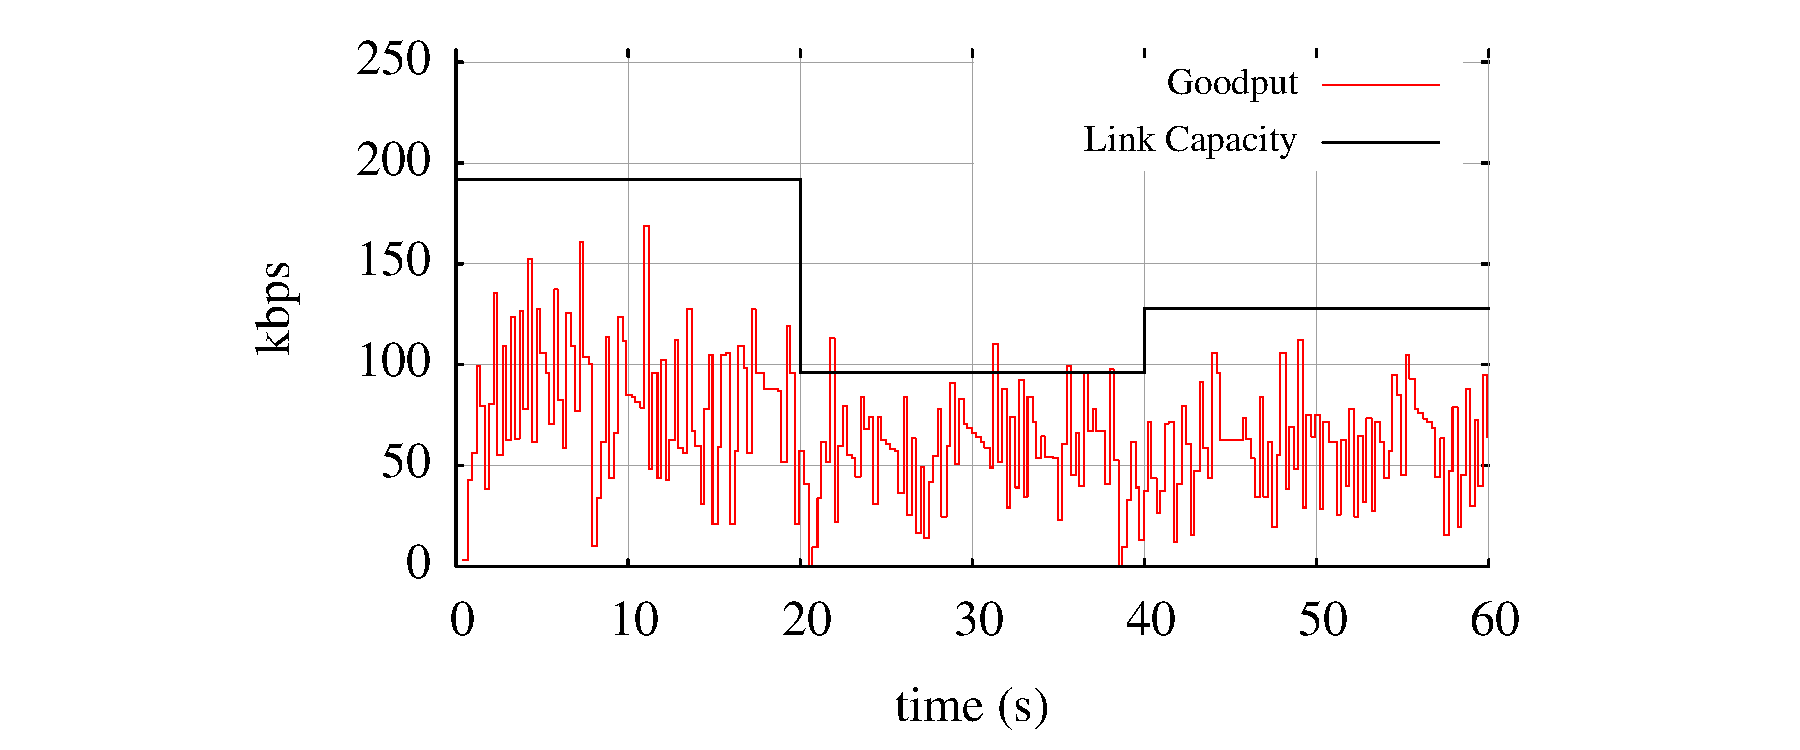
\includegraphics[width=0.5\textwidth, clip=true, trim=3cm 0 4.5cm 0]
      {chap5_graph_sl_tfrc}
    }
    \subfloat[TFRC]{
      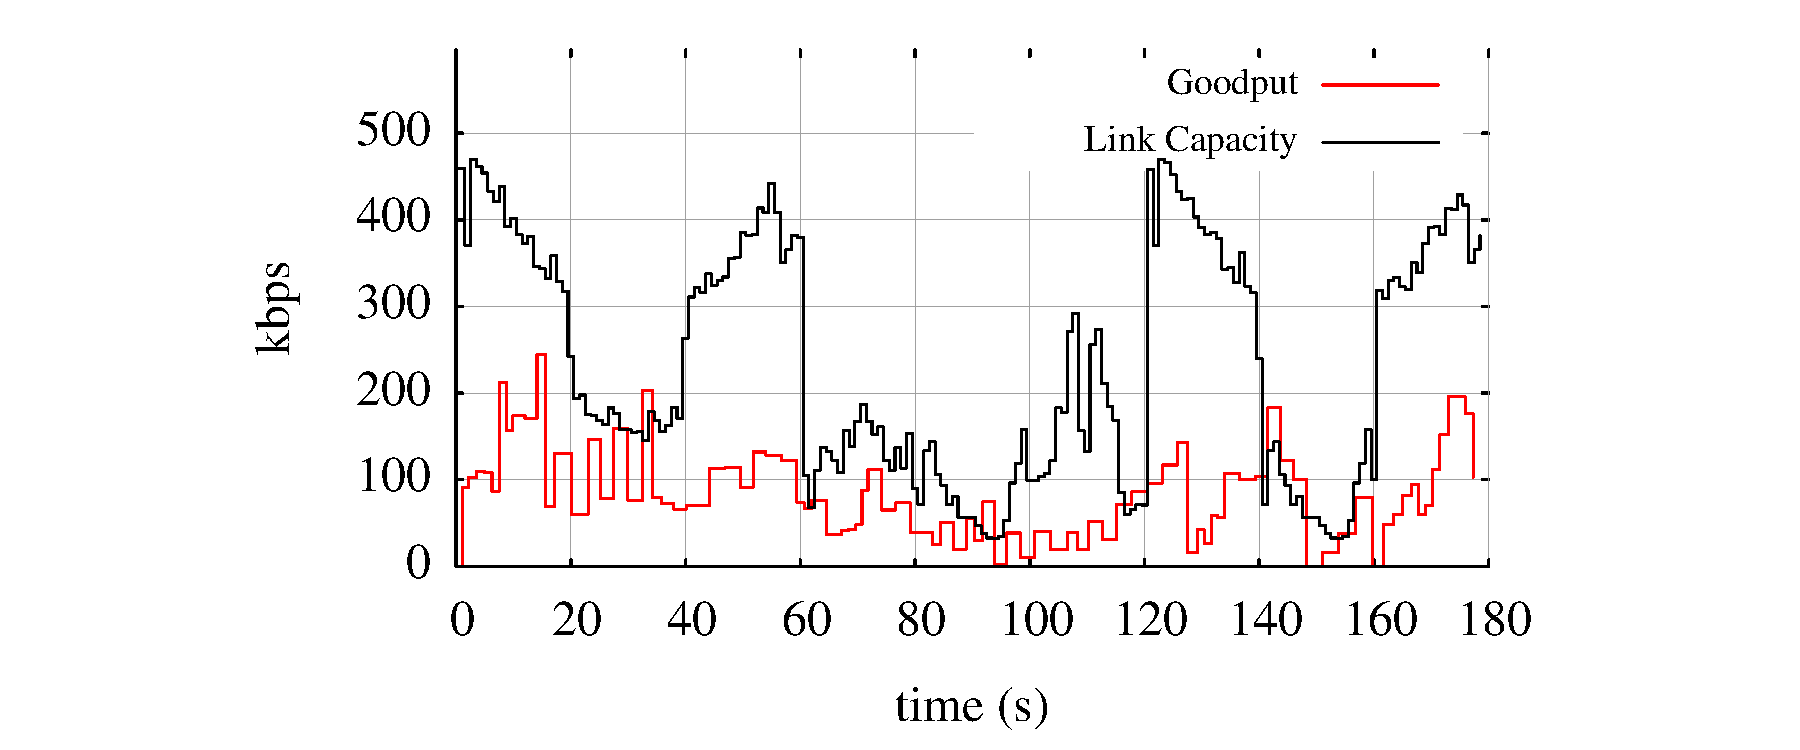
\includegraphics[width=0.5\textwidth, clip=true, trim=3cm 0 4.5cm 0]
      {chap5_graph_3g_tfrc_1}
    }
  }
  \centerline{
    \subfloat[TMMBR]{
      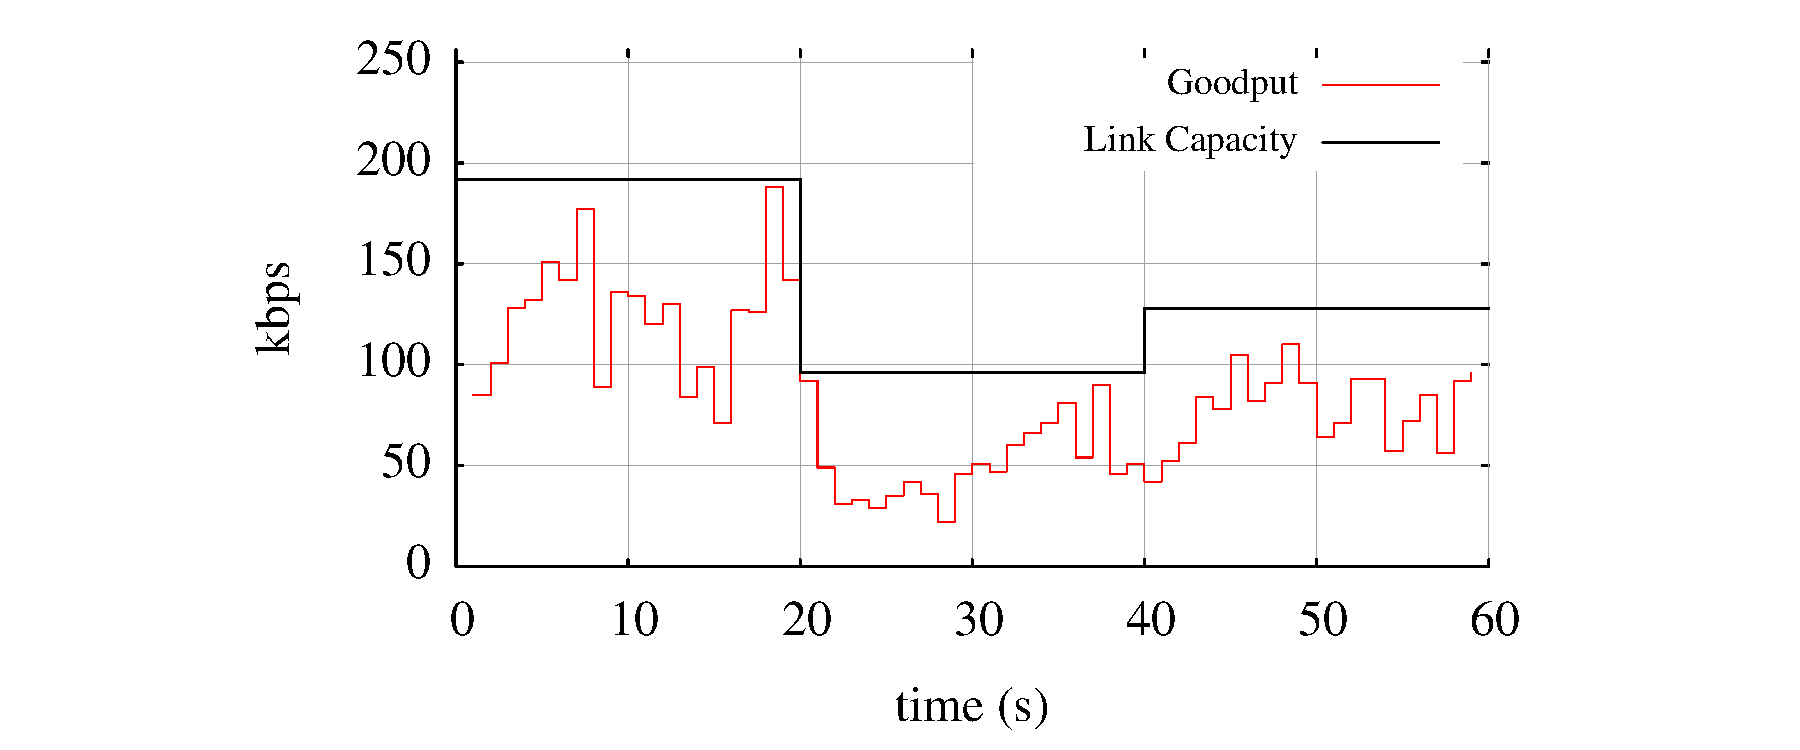
\includegraphics[width=0.5\textwidth, clip=true, trim=3cm 0 4.5cm 0]
      {chap5_graph_sl_tmmbr}
    }
    \subfloat[TMMBR]{
      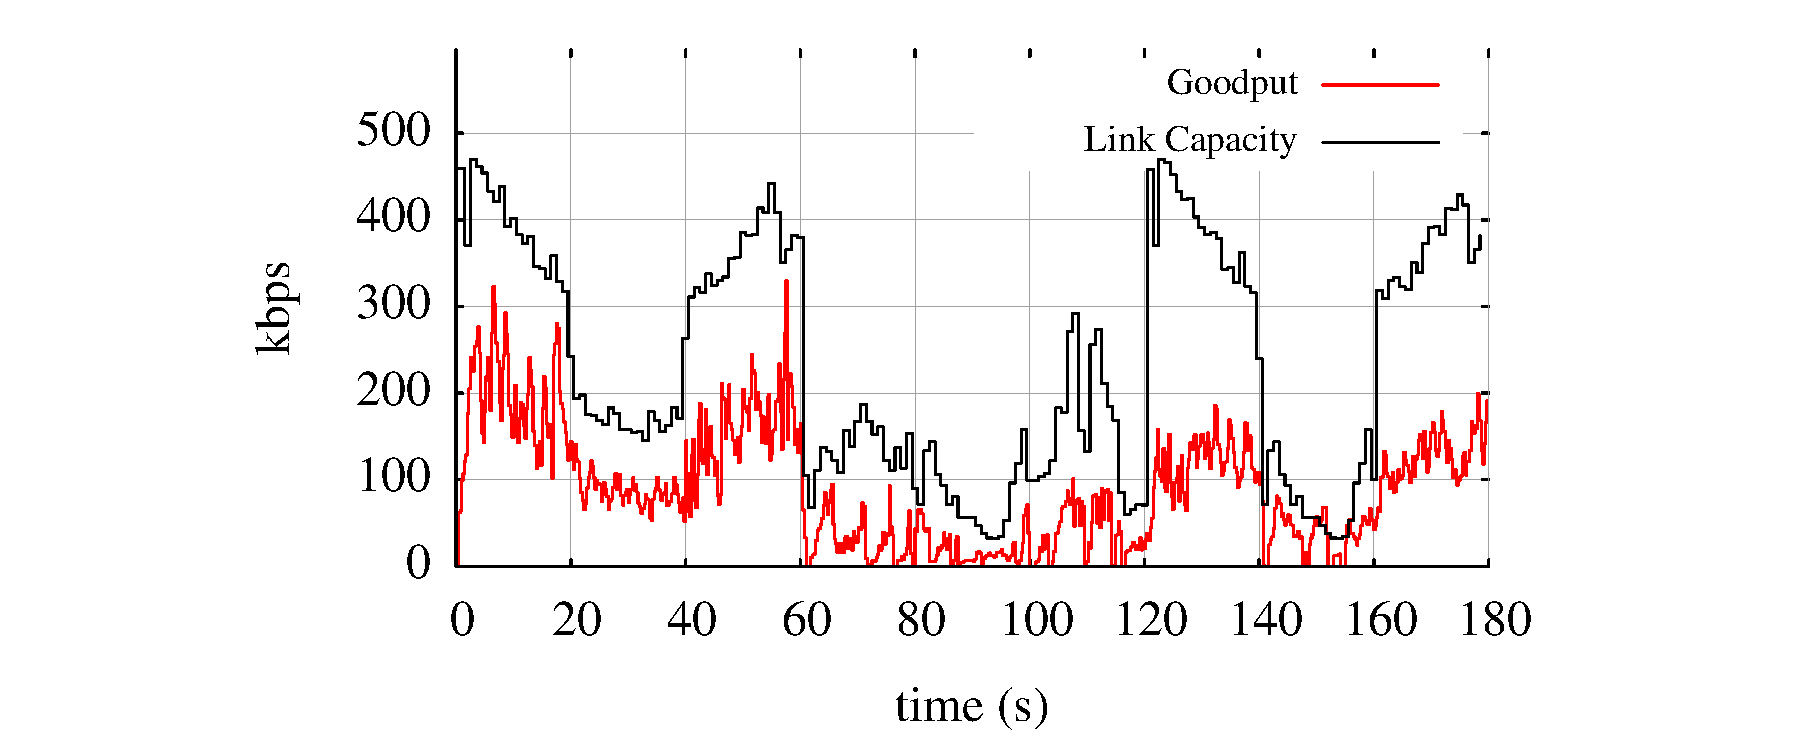
\includegraphics[width=0.5\textwidth, clip=true, trim=3cm 0 4.5cm 0]
      {chap5_graph_3g_tmmbr_u}
    }
  }
  \centerline{
    \subfloat[C-NADU]{
      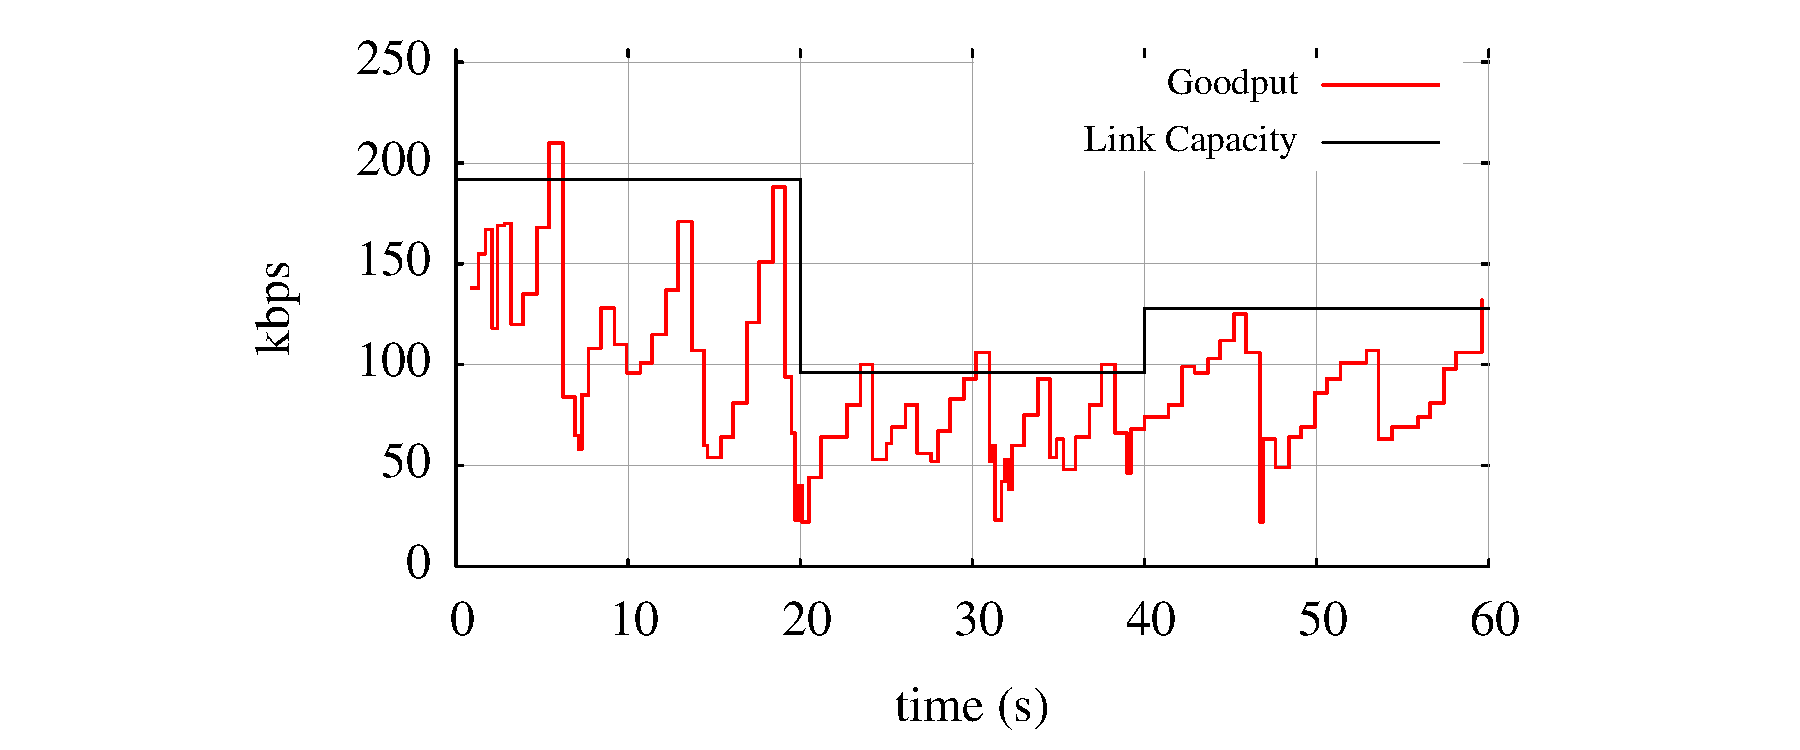
\includegraphics[width=0.5\textwidth, clip=true, trim=3cm 0 4.5cm 0]
      {chap5_graph_sl_cnadu}
    }
    \subfloat[C-NADU]{
      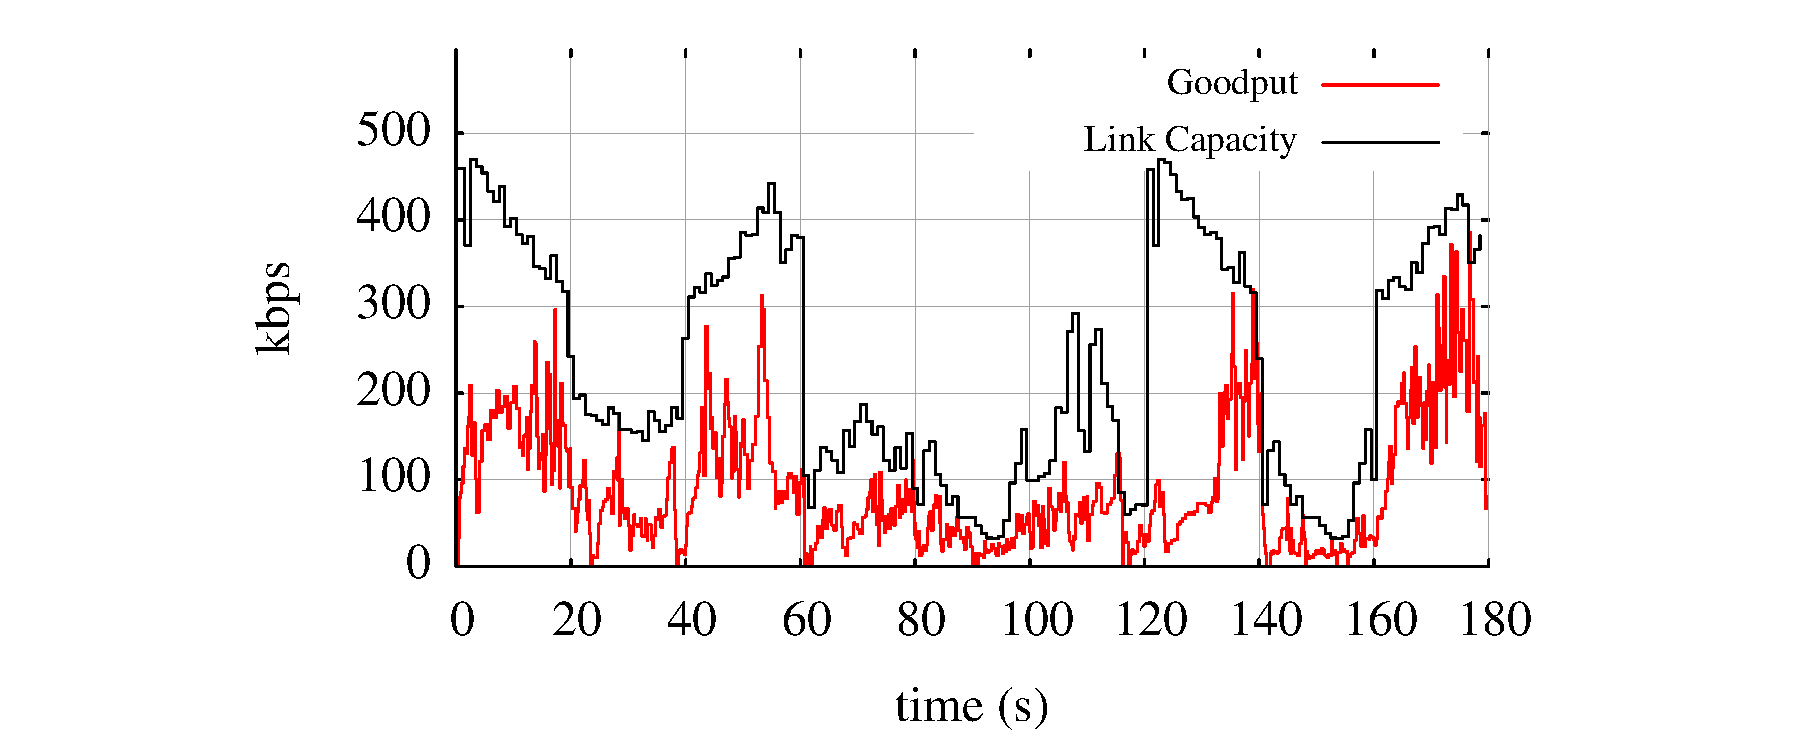
\includegraphics[width=0.5\textwidth, clip=true, trim=3cm 0 4.5cm 0]
      {chap5_graph_3g_cnadu}
    }
  }
  \caption{TPerformance of TFRC, TMMBR and C-NADU in a slow
  time-varying link (a, c, e) and 3G network (b, d, f).}
  \label{fig:3grc}
\end{figure}


\begin{table}[!t]
\centering{
\begin{tabular}{cccc}
\hline
 & $Goodput_{avg}$ & PLR & $PSNR_{avg}$\\
 & (kbps)  &(\%) & (dB)\\
\hline
TFRC & 84.1 & 6.9\,\%& 29.3 \\ %
TMMBR & 89.8 & 3.7\,\% & 30.5 \\ %
%NADU & 106 & 93 & 29.9& 6.3\%\\%
C-NADU & 92 & 2.2\,\% & 31.9 \\%
\hline
\end{tabular}
}
\caption{Comparing TFRC, TMMBR, C-NADU for calls over mobile nodes (180\,\emph{s}
simulations using 3G traces).}
\label{table:3grc}
\end{table}

\section{Performance Analysis of TFRC, TMMBR, C-NADU, and RRTCC}

This section briefly discusses the performance of each congestion control
algorithm. The detailed analysis can be found in the respective papers.

Our results in \citepub{c:3grc} show that TFRC produces a sawtooth sending
rate, similar to the performance in~\cite{saurin:2006:thesis}. When the media
stream is the only flow on the end-to-end path, we also observe that the average
bandwidth utilization (ABU) is between 30-40\,\%, i.e., TFRC under utilizes the
link and the loss ratio is about 6\,\%, which results in a lower media quality
(approximated by measuring PSNR) compared with the other two schemes (see
Table~\ref{table:3grc}). TMMBR-based congestion control utilizes the link
better than TFRC (ABU between 50-70\,\%) and produces a lower loss ratio
($\approx$3\,\%). Lastly, C-NADU has comparable bandwidth utilization
(ABU=55-60\,\%) and loss ratio ($\approx$2\,\%) to TMMBR.
Figure~\ref{fig:3grc} shows the performance of TFRC, TMMBR and C-NADU over two
types of bottleneck links, a slow time-varying link and a 3G link.


\begin{figure}[!t]
\centerline{
%\hfill
\subfloat [Call 1 vs Call 2] {\label{fig_sim-mixed-1-1}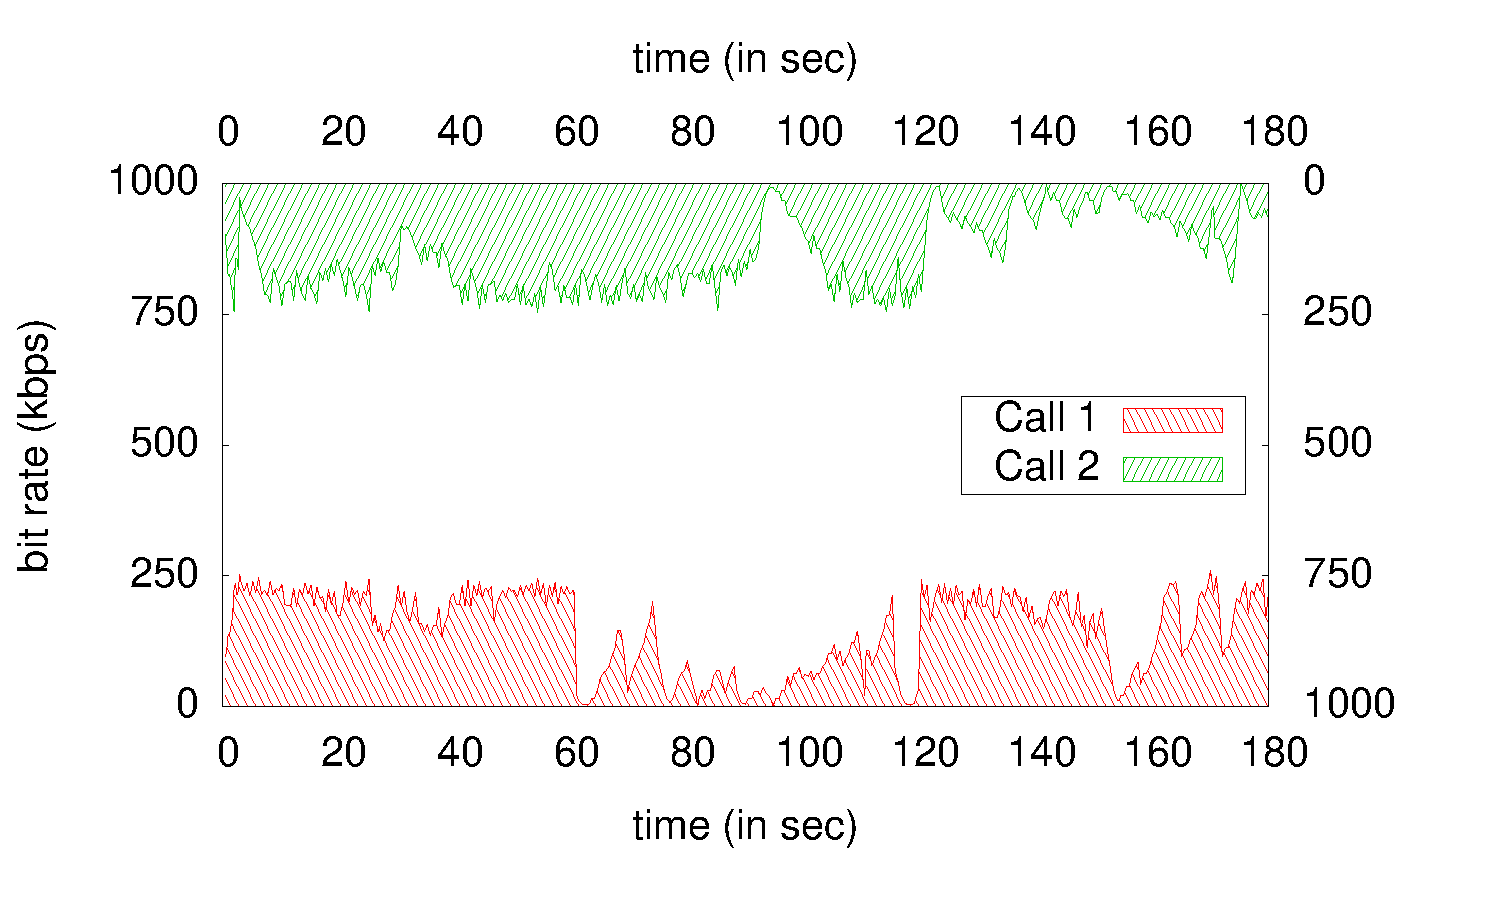
\includegraphics[width=0.5\textwidth]{chap5-graph-5rtp_uc1_12}%
}
%\hfill
\subfloat [Call 1 vs Call 3] {\label{fig_sim-mixed-1-2}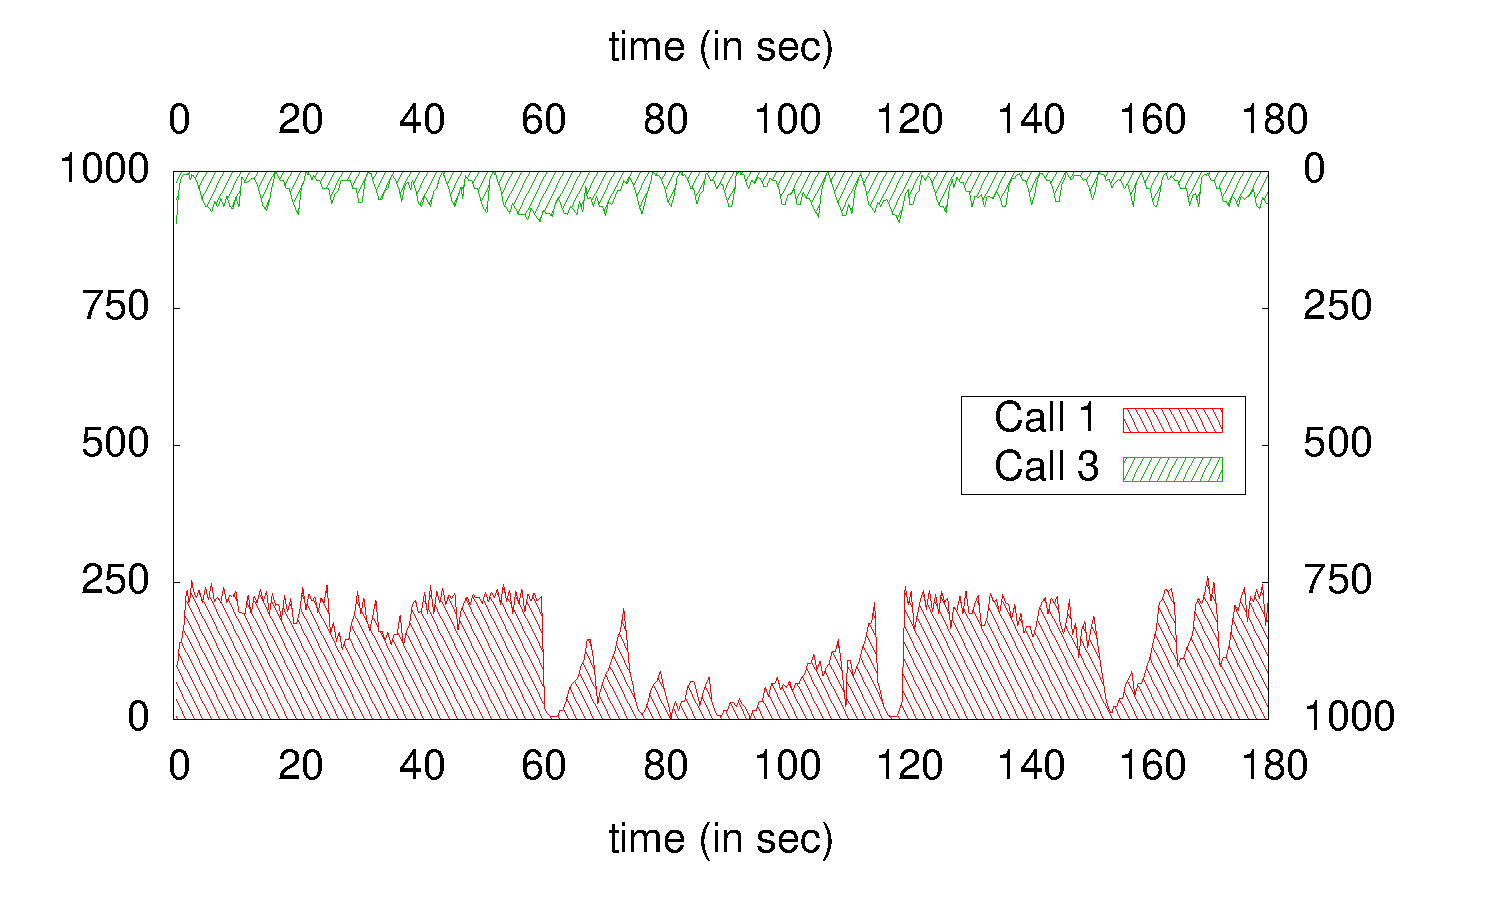
\includegraphics[width=0.5\textwidth]{chap5-graph-5rtp_uc1_13}%
}
%\hfill
}
\centerline{
%\hfill
\subfloat [Call 1 vs Call 4] {\label{fig_sim-mixed-1-3}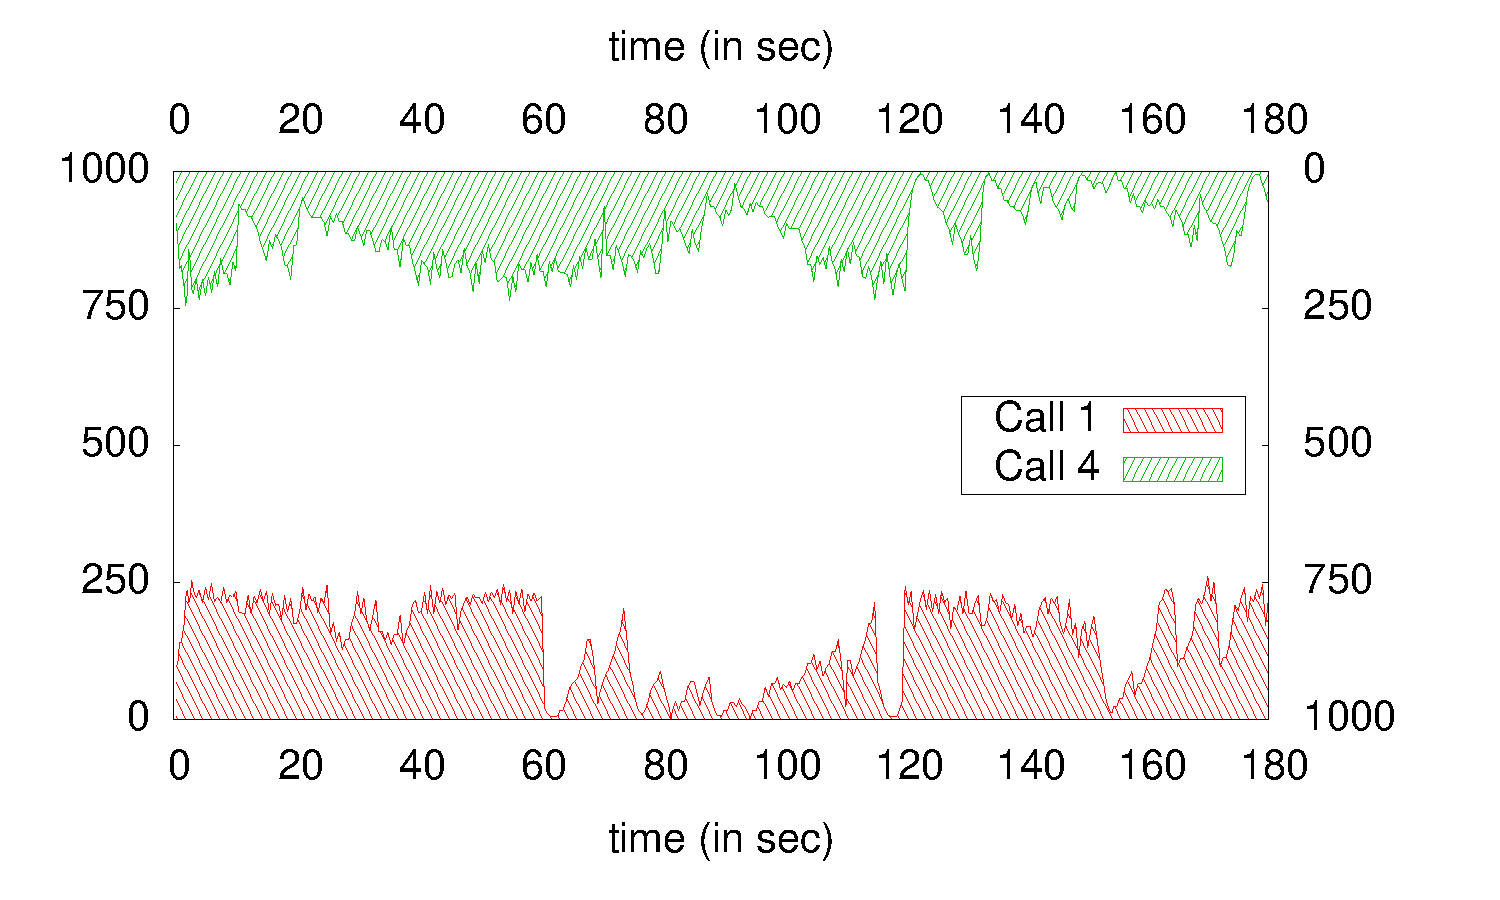
\includegraphics[width=0.5\textwidth]{chap5-graph-5rtp_uc1_14}%
}
%\hfill
\subfloat [Call 1 vs Call 5] {\label{fig_sim-mixed-1-4}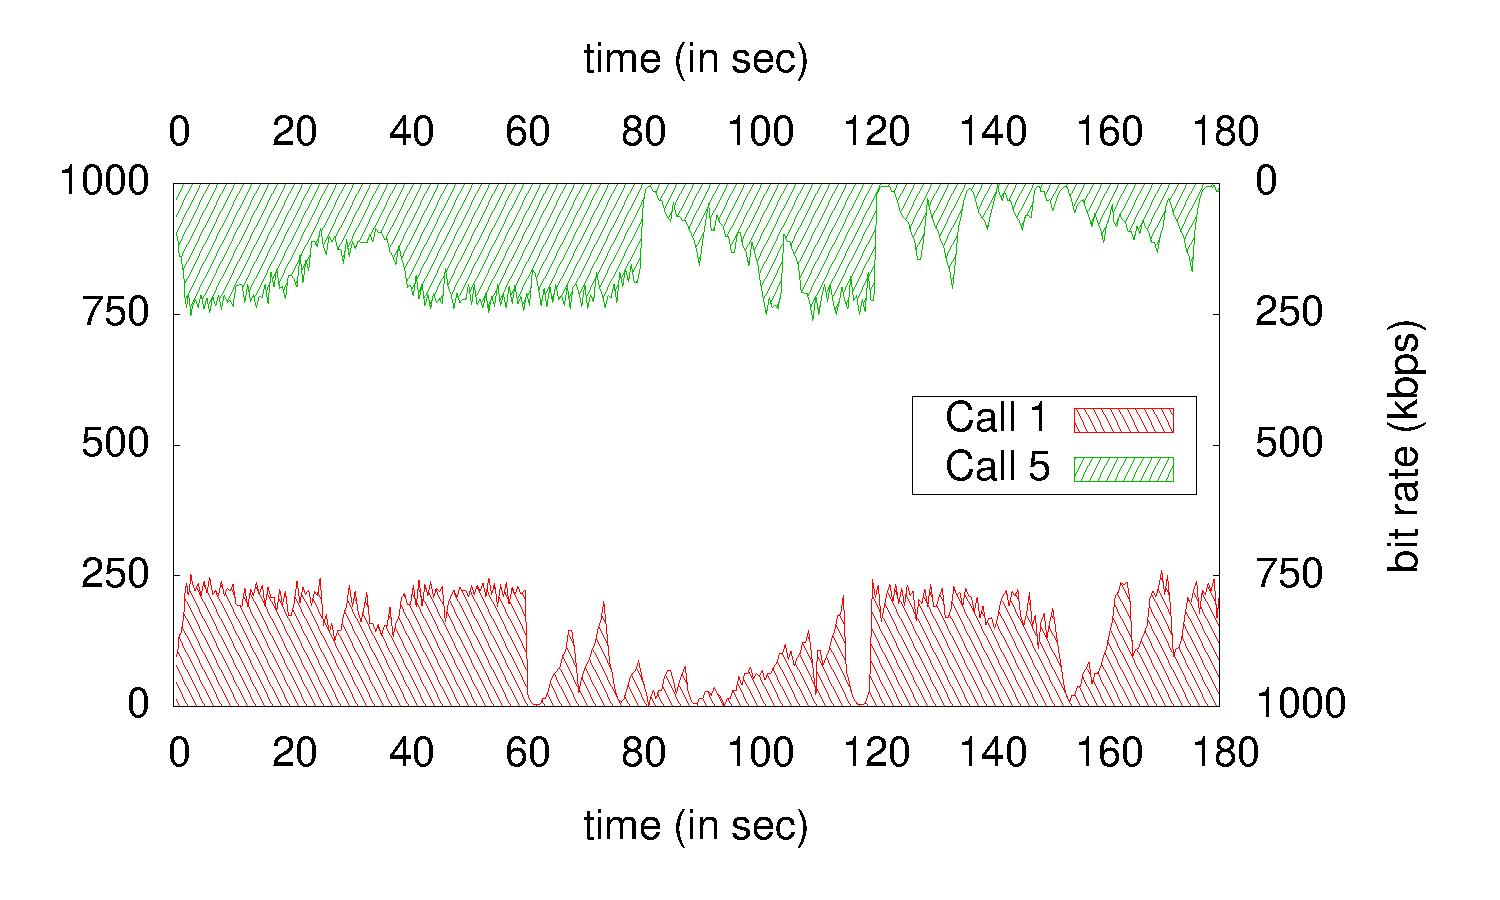
\includegraphics[width=0.5\textwidth]{chap5-graph-5rtp_uc1_15}%
}
%\hfill
}
\caption{Performance of five C-NADU calls competing for
capacity on a shared bottleneck in a heterogeneous network. Each call needs
to quickly adapt to changes in 3G link capacity and fairly share the
bottleneck link.}
\label{fig:hetrc}
\end{figure}

\begin{table}[!t]
\centering{
\scalebox{0.9}{
\begin{tabular}{cccccc}
\hline
 & 3G Capacity & $Goodput_{avg}$ & PLR & $PSNR_{avg}$ & ABU \\
 & Pattern & (kbps) & (\%) & (dB) ($\sigma$)  & (\%) \\ 
\hline
Call 1 & Excellent-Poor-Elevator & 140.10 & 2.15\,\% & 31.4 ($0.39$) & 70.1\,\% \\ 
Call 2 & Good-Good-Poor & 133.55 & 1.61\,\% & 31.9 ($0.62$)& 66.8\,\% \\ 
Call 3 & Poor-Poor-Poor & 35.18 & 1.55\,\% & 22.2 ($1.13$)& 17.59\,\% \\ 
Call 4 & Fair-Fair-Poor & 114.96 & 2.75\,\% & 31.1 ($0.75$)& 57.5\,\% \\ 
Call 5 & Excellent-Elevator-Poor & 130.23 & 2.25\,\% & 31.3 ($0.13$)& 65.1\,\% \\ 
\hline
\end{tabular}
}}
\caption{C-NADU: Five calls in a heterogeneous network with end-to-end latency
between 60-120\,\emph{ms} and 0.5\,\% link-layer losses.}
\label{table:hetrc}
\end{table}

In \citepub{c:hetrc}, we show that C-NADU is self-fair with other C-NADU flows
in both wired and wireless environments~\cite{singh:2010.thesis}, and in
\citepub{c:fecrc} we show that it competes fairly with TCP cross-traffic, for both
the long- and short-TCP flows. Figure~\ref{fig:hetrc} show five video calls in which
each sender uses an independent 3G link into a common bottleneck to the
receivers. The 3G links are based on radio link traces and have different
capacities. Hence, at some instances of time, the 3G link is the constraint and
at other times it is the shared bottleneck link. Table~\ref{table:hetrc} shows that
four calls have comparable performance (see PSNR and goodput) and one call suffers
due to poor connectivity (the 3G link has insufficient capacity which affects
the quality).

\begin{figure}[!t]
  \centerline{
    \subfloat{
      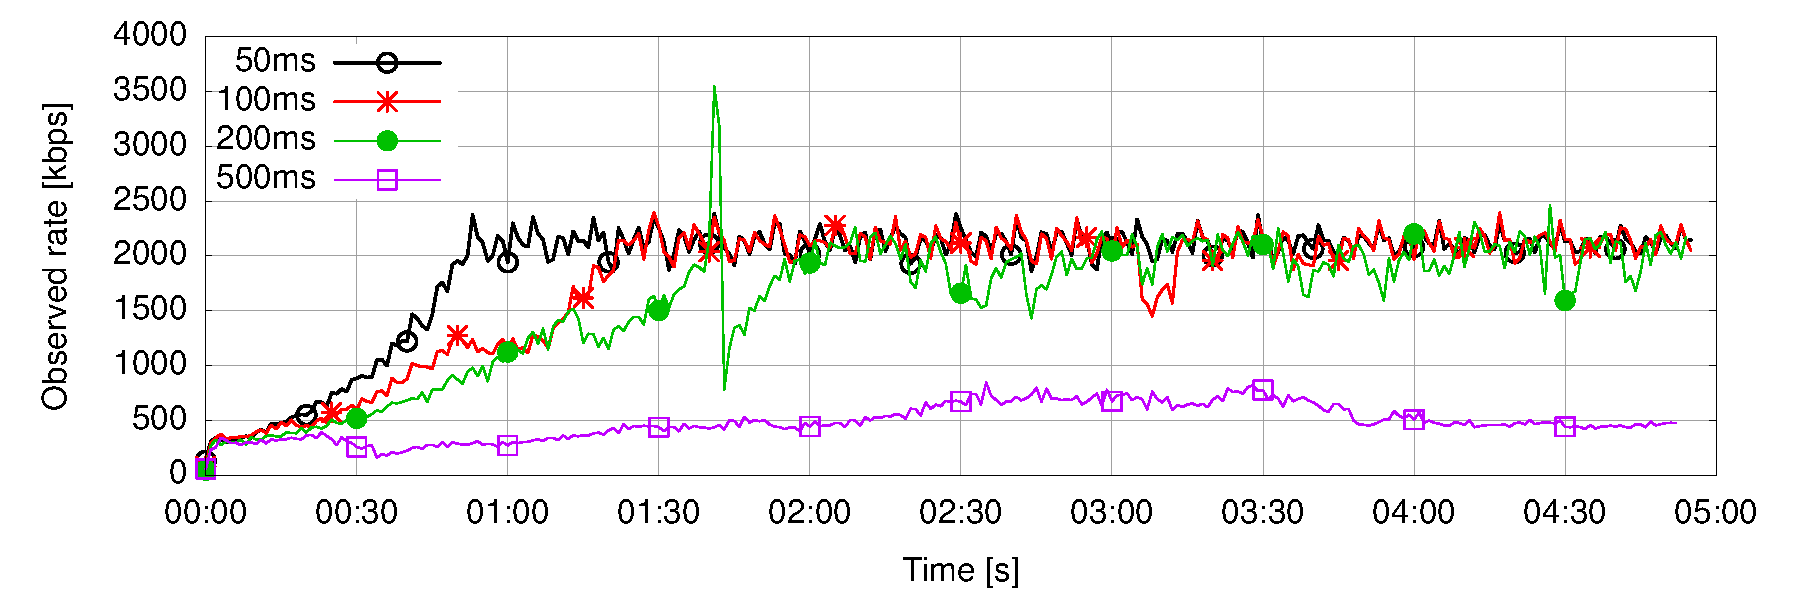
\includegraphics[width=0.8\textwidth]
      {chap5-graph-rrtcc-latency}
    }
   }
   \centerline{
    \subfloat{
      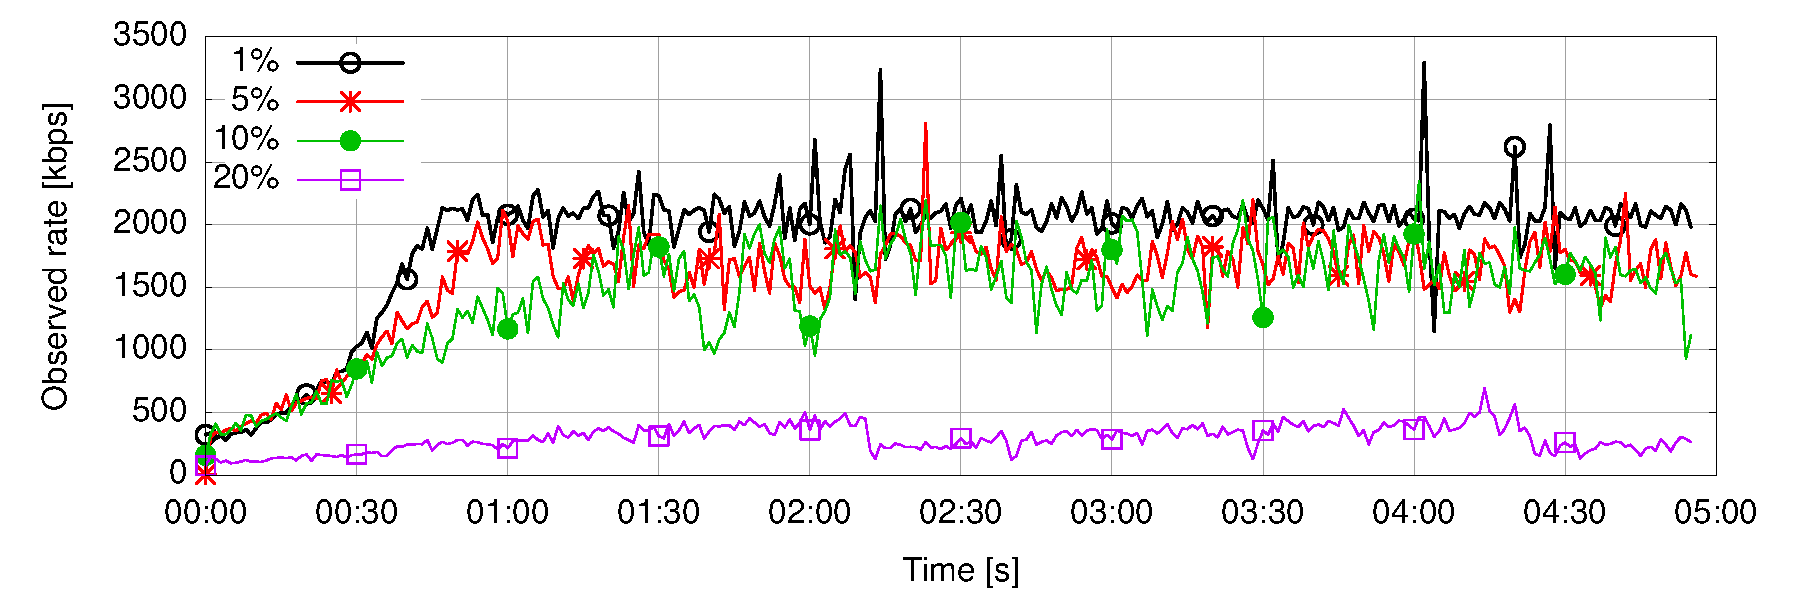
\includegraphics[width=0.8\textwidth]
      {chap5-graph-rrtcc-plr}
    }
  }
  \caption{The plots show the performance of RRTCC on a link with varying
  delay and fractional loss rate. We observe that by the sending rate
  decreases with increasing link latency or bit-error loss. }
  \label{fig:rrtcc-single}
\end{figure}

\begin{table}[!t]
\begin{center}{
  \scalebox{0.9}{
\begin{tabular}{ ccccc }
\hline
 & $Goodput_{avg}$ & Residual  & PLR\\
 & (kbps)  & Loss (\%) & (\%)\\
\hline
 0\,\% & 1949.7 $\pm$ 233.62 & 0.011 & 0.011 \\ 
 5\,\% & 1568.74 $\pm$ 178.52 & 0.23 & 9.77 \\ 
 10\,\% & 1140.82 $\pm$ 161.92 & 0.49 & 19.02 \\ 
 20\,\% & 314.4 $\pm$ 61.98 & 2.43 & 36.01 \\ \hline
\end{tabular}
}}
\end{center}
\caption{RRTCC: Metrics for a bottleneck with different packet loss rates.}
\label{tab:rrtcc-loss}
\end{table}

In \citepub{c:eval}, we evaluate the performance of RRTCC in several
scenarios: by itself on a bottleneck link, competing with other RRTCC flows
and competing with TCP cross-traffic. Figure~\ref{fig:rrtcc-single} shows an
example plot of the performance of RRTCC. In Figure~\ref{fig:rrtcc-single}(a) when
increasing the bottleneck link latency reduces the sending rate of RRTCC.
Similarly, Figure~\ref{fig:rrtcc-single}(b) shows that when increasing the loss
rate also affects the sending rate. However, Table~\ref{tab:rrtcc-loss} shows
that even though the link has a high loss rate, the residual loss rate is low
(even when the loss was 20\,\%), mainly due to the use of NACKs, PLI and FEC.


\begin{figure}[!t]
\centerline{
  \subfloat[Start together]
    {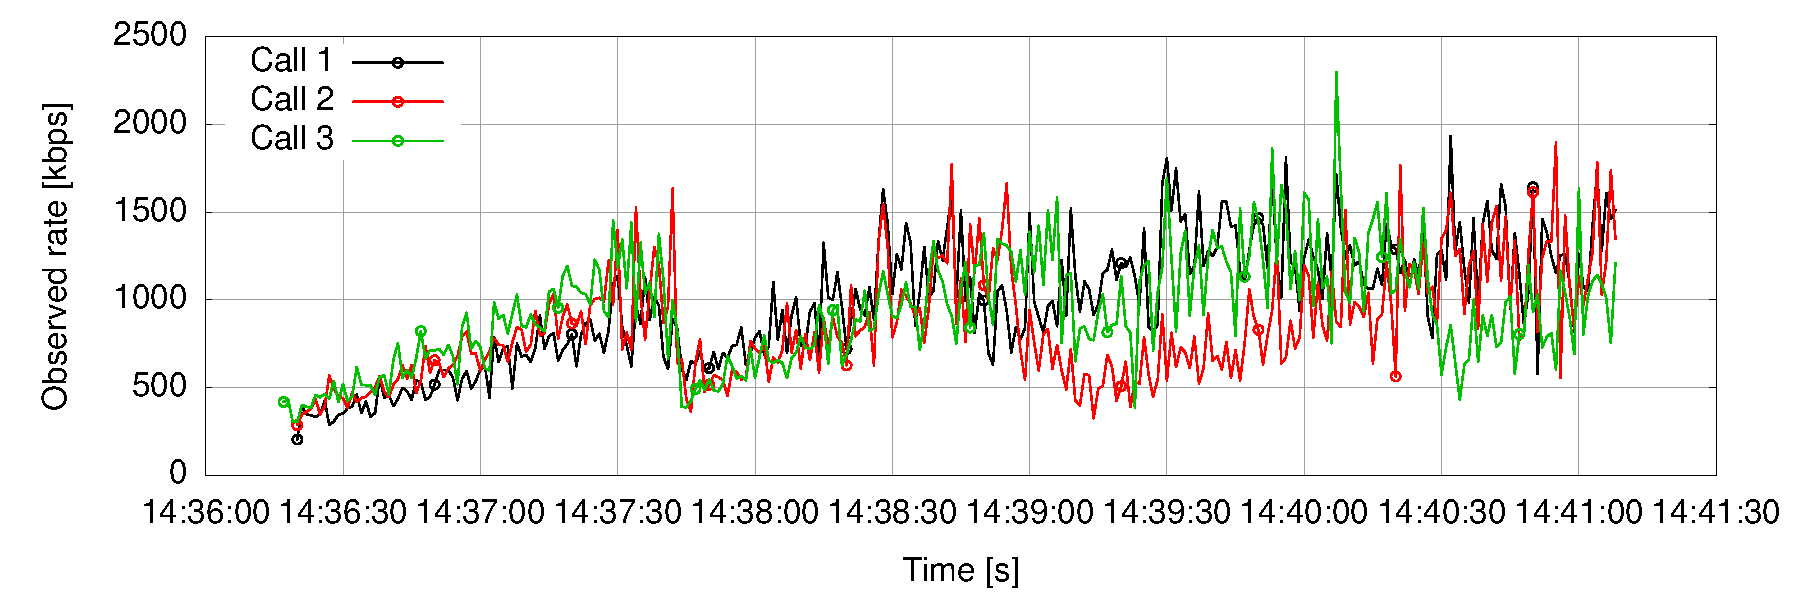
\includegraphics[width=0.8\textwidth]
    {chap5-graph-rrtcc-three-calls-sync}}
  }
  \centerline{
  \subfloat[Start 30\,\emph{s} apart]
    {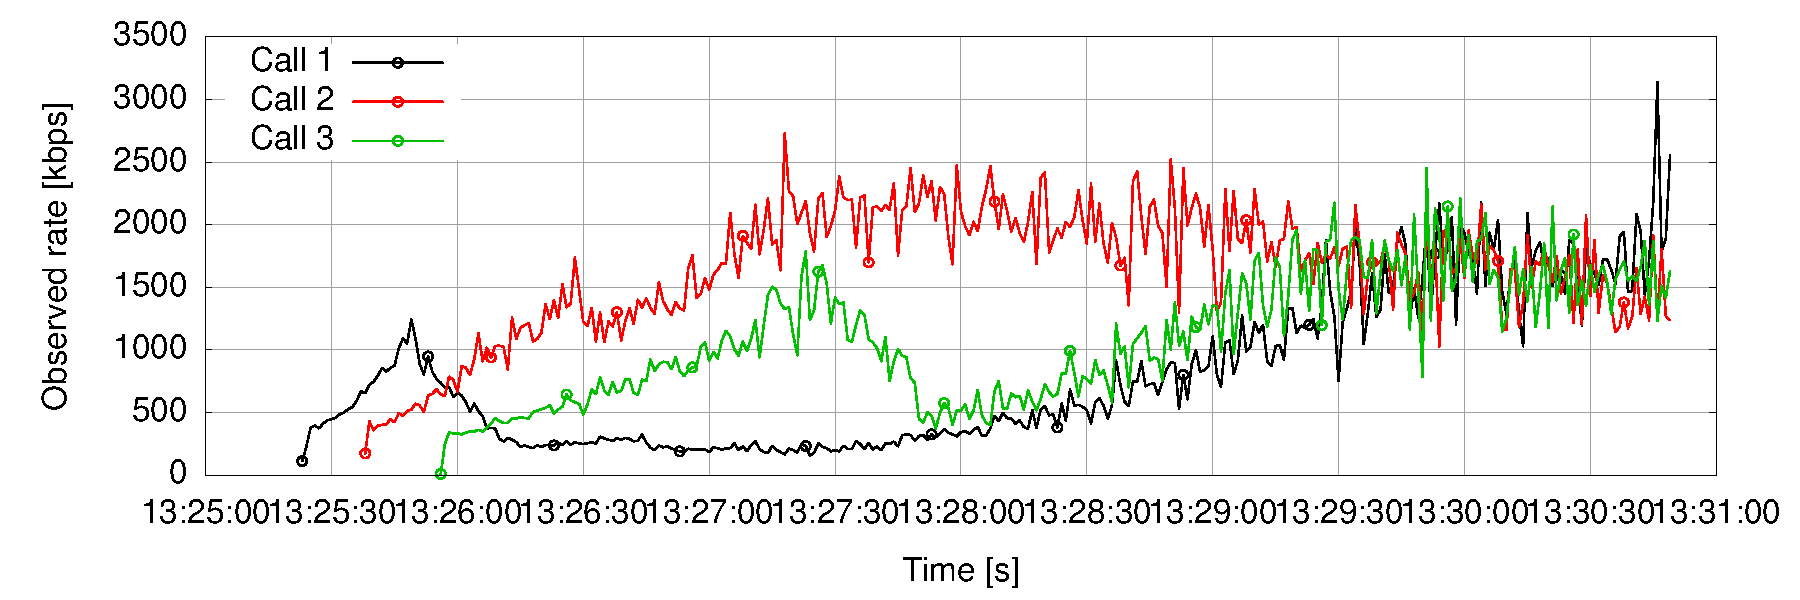
\includegraphics[width=0.8\textwidth]
    {chap5-graph-rrtcc-three-calls-async}}
  }
   \caption{The plots show the variation in receiver rate of three RRTCC
   flows, a) starting together, b) starting 30\,\emph{s} apart. The total duration of
   the call is 5 mins (300\,\emph{s}).}
\label{fig:rrtcc-self-fair}
\end{figure}

\begin{table}[!t]
\begin{center}
  \scalebox{0.9}{
\begin{tabular}{ccccc}
\hline
& $Goodput_{avg}$  & RTT & Residual & PLR\\
& (kbps)& (ms) & Loss (\%) & (\%)\\ \hline
 3 calls &  809.07 $\pm$ 202.38 &   31.48 $\pm$ 24.93 & 0.21 & 0.23 \\  
 3 calls (time shifted) &  1154.32 $\pm$ 250.54 &   35.15 $\pm$ 27.88 & 0.08 & 0.91 \\ \hline
\end{tabular}
}
\end{center}
    \caption{RRTCC competing with similar cross-traffic on the bottleneck link.}
    \label{tab:self-fair}
\end{table}

Next, we emulate three calls sharing a common bottleneck. In this case, the
individual media rates do not reach their individual maximum rate of 2\,\emph{Mbps}.
Figure~\ref{fig:rrtcc-self-fair}(a) shows that the three calls ramp up at about the
same rate, reach a peak and drop their rate simultaneously. The sending rates
synchronize, even though the flows originate from different endpoints using
independent RTP stacks.

Lastly, instead of the three calls starting together, each call starts at 30\,\emph{s}
intervals. We observe that while the media rate per call on average is higher,
the first call has a disadvantage. In all the cases, the first media flow temporarily 
starves when a new flow appears, ramping up again after a few minutes.
Figure~\ref{fig:rrtcc-self-fair}(b) shows the instantaneous rates of each of
the calls. The first call temporarily starves when new flows appear because,
when it starts, it is the only flow on the bottleneck and does not encounter
any queues; it observes a certain RTT and uses that as the baseline. When the
second flow appears, the second flow already observes queues from the existing
stream and competes with it, while the initial flow observes an increase in
queues and reduces the sending rate to avoid congestion.


To summarize, we observe that the performance of TFRC is bursty, which may
lead to poor user-experience, whilst TMMBR, C-NADU and RRTCC have a more
stable throughput. Lastly, TMMBR appears to be conservative with very low
packet loss, while RRTCC appears to be aggressive with a lot more packet loss.
C-NADU appears to be in between the two schemes, with higher throughput than
TMMBR and much lower packet loss compared to RRTCC. 

\section{Summary}

In this chapter, we describe congestion control implemented using congestion
cues from in-band sources and signaled in path (in RTCP). We further
categorize the congestion control algorithms based on \emph{where they are
implemented}: sender-driven scheme (e.g., TFRC), receiver-driven scheme (e.g.,
TMMBR), or co-operative scheme (combination of sender and receiver, e.g.,
C-NADU, RRTCC) and compare the performance of algorithms in each scheme. Our
initial experiments show that that C-NADU or TMMBR would be preferred, but
requires further investigation with more complex aggregate flows (mainly short
or bursty TCP flows).

In the next chapter, we discuss the interaction between the error-resilience
algorithm and the congestion control algorithm and evaluate if FEC can be used
as a probing mechanism by a multimedia congestion control algorithm.

%% An example for changing the running header (the optional parameter)

 \chapter{Interaction of Error-Resilience and Congestion Control}
 \label{chap:er-cc}
Error-resilience is typically a topic discussed orthogonally to congestion
control, mainly because error-resilience caters to handling
packet loss while congestion control caters to the amount of information sent
over the network. This chapter is based on our work on unifying
error-resilience and congestion control, which is documented in 
\citepub{c:err}, \citepub{c:fecrc}, and \cite{draft.adaptive.fec}.

In \citepub{c:err}, we evaluate the performance of the various
error-resilience schemes available for use in interactive multimedia
communication (mainly applicable to H.264). These are: using Negative
Acknowledgement (NACK) or Packet Loss Indication (PLI), Forward Error
Correction (FEC) or Unequal Level of Protection (ULP), adaptive slice sizes,
and Reference Pictures Selection Indication (RPSI). We evaluate the
performance of the proposed mechanisms in diverse scenarios in a simulated
environment (in ns-2) using real-world 3G loss patterns~\cite{3gppSim}.
Lastly, based on our observations, we define the applicability of the various
error-resilience with respect to end-to-end latency and packet loss.

In \citepub{c:fecrc}, we propose using FEC not only for error-resilience but
also for congestion control, i.e., instead of probing for available capacity
by increasing the sending rate of the media stream, the endpoint sends
redundant packets. If a packet gets lost and the added FEC packet arrives in
time, the receiving endpoint would recover the lost packet. However, if the
packet is not lost, by introducing the FEC packet the sender not only
discovers that there is additional available capacity, but also has a sense of
the (minimum) magnitude of the available capacity. We compare our proposal
with our previous work in \citepub{c:3grc} and \citepub{c:hetrc}, and 
RRTCC~\cite{draft.rrtcc}. We evaluate the performance of the
mechanisms in diverse scenarios implemented in a simulation environment (in
ns-2) and in our testbed.

\section{Error-resilience Schemes}
% explain all 4 and the adaptivity

H.264~\cite{h264} uses various error-control methods~\cite{err_res_h264_std,
wang98error, wang00review, 310669} to overcome loss due to corruption (e.g.,
in wireless) and non-bursty packet loss (e.g., due to congestion). These
methods are classified into three categories: source coding, channel coding,
and joint source and channel methods. Source coding refers to the methods
implemented by the video codec. Channel coding refers to the methods
implemented by the networking layer. Joint source-channel refers to methods
that combine source-coding and network-coding mechanisms.

The H.264/AVC codec has several features that support error-resilient
mechanisms for video communication that correspond to the above
categorisation~\cite{310669}. At the codec level, the following are available:
adaptive slice size, Reference Picture Selection (RPS), and Flexible
Macroblock Ordering (FMO)~\cite{err_res_h264_std, wenger_ott_jscc}. Similarly,
at the channel level, the following are available: Selective Retransmission
(NACK), and PLI. An example of joint source-channel is UEP with 
FEC~\cite{wang00review}, in which the sender
attempts to selectively protect important parts of the bitstream or 
encodes redundant frames differently than other frames~\cite{ervcuupkp}.
% pictures -> frames

The performance of the available error-resilience mechanisms vary with the
observed end-to-end latency, link loss, bandwidth constraints and operating
environment (3G/LTE to 3G/LTE, 3G/LTE to WLAN, or wireless to fixed, etc.). No
single error repair mechanism fits all operating environments. A solution that
works for an observed packet loss ratio of less than 2\,\%, may not scale well
for paths with higher packet loss or higher latency.

% The combination of end-to-end delay requirements, capacity constraints and
% varying packet loss rate require different error resilience mechanisms.

\begin{figure}
\centerline {
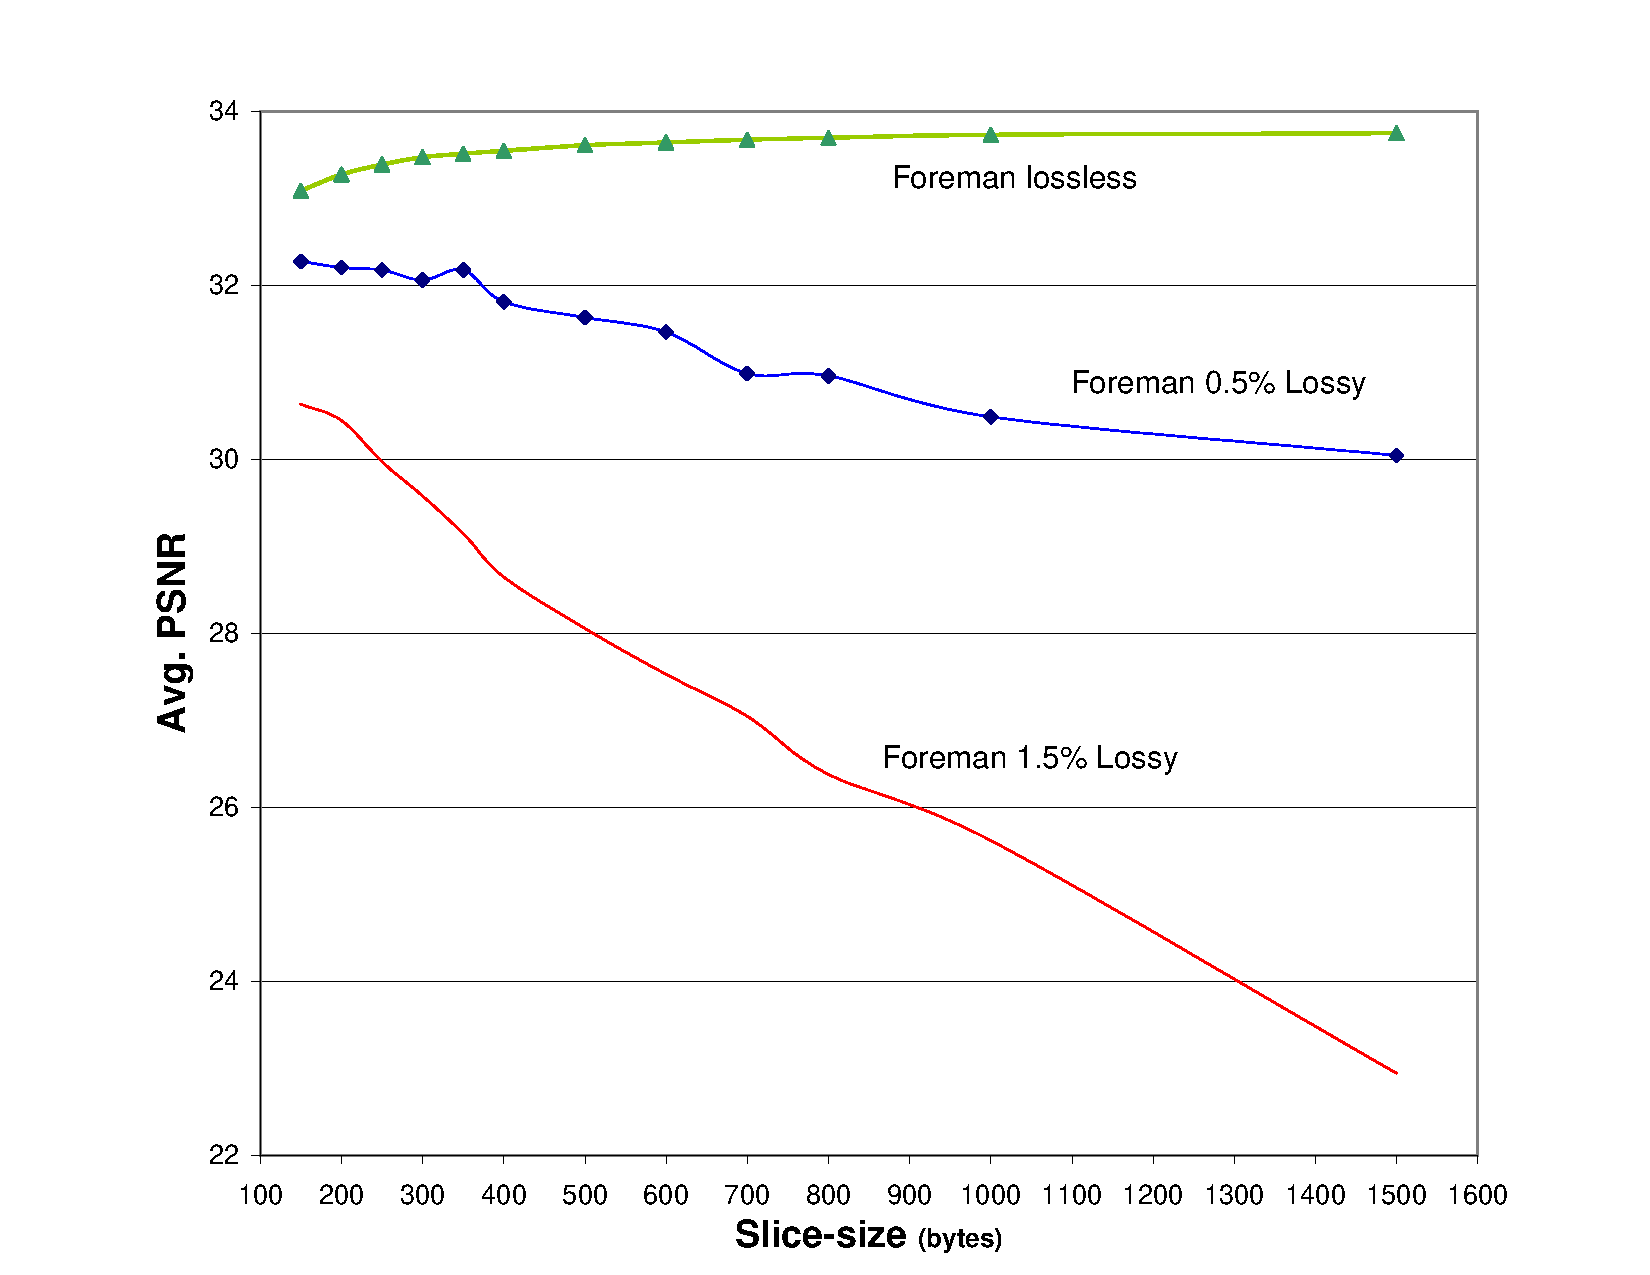
\includegraphics[width=0.66\textwidth]{chap6-graph-slicesize_mot}
}
\caption{Effect of different slice sizes on PSNR for links experiencing different amounts of bit-error corruption.}
\label{fig:slicesize_mot}
\end{figure}

\begin{itemize}
\setlength{\itemsep}{0pt}

  \item \textbf{\texttt{Retransmissions}}: In RTP, retransmissions are either
  payload-specific or at the transport-specific. Transport-specific loss
  contains packet loss information (Generic NACK), while payload-specific loss
  contains Slice Loss Information (SLI), Picture Loss Information (PLI) or
  Reference Picture Selection indication (RPS). Typically, the receiver
  detects a loss and sends it as soon as the RTCP reporting interval allows
  feedback.

  \item \textbf{\texttt{Adapting Slice Sizes}}: the encoder adapts the size of
  the picture slice based on the link characteristics; when the channel is
  lossless there can be one picture per slice (up to the MTU size) and when
  high losses are reported, the slices are reduced in size (up to 100 bytes).
  Larger slice sizes improve encoding efficiency, but are more vulnerable to
  frame losses. Figure~\ref{fig:slicesize_mot} shows the variation of average
  PSNR with respect to different slice sizes in varying loss scenarios. We
  observe that there is a direct correlation between packet loss, slice
  size and media quality.

  \item \textbf{\texttt{Reference Picture Selection}}: Instead of
  retransmitting a lost packet, the encoder finds the list of correctly
  received pictures (or frames) by the decoder. Hence, for subsequent encodings, the
  encoder uses a different decoded picture for inter-prediction reference.
  This method stops the temporal error propagation caused by an earlier packet
  loss. In the RPS message, the decoder reports the list of pictures (or frames)
  that were correctly received or lost. Hence, the encoder is able to retrieve
  the lost picture data. The mode of operation can be decided
  depending on the observed packet loss rate.

  \item \textbf{\texttt{Unequal Error Protection}}: When the link latency is
  high, retransmissions cannot be used because the
  retransmitted packets arrive too late to be played back. In these cases, the
  sender proactively uses a portion of the available capacity to send
  redundant packets (typically, FEC), hoping to recover any lost packet before
  decoding. Hence, by using UEP, the media senders try to strike a balance by
  protecting only a chosen set of the media packets. In \citepub{c:err}, we
  protect the reference frames and not the non-reference frames with UEP.

\end{itemize}

In \citepub{c:err}, we stream three different YUV sequences~\cite{YUV_seq} over a
3G link simulated in \emph{ns-2}~\cite{ns2} with varying amount of link layer
packet loss (0.5\,\%, 1.0\,\% and 1.5\,\%)~\cite{3gppSim}. Our experiments
show that using NACK, the endpoint is able to correct 15-30\,\% of the lost
packets for an end-to-end path latency of 60\,\emph{ms}, which meets the
preferred  packet latency of 150\,\emph{ms} specified by ETSI~\cite{etsi.qoe}.
The number of recovered packets will increase with shorter RTCP reporting
intervals; in this paper, we use a 1\,\emph{s} reporting interval, with early and
immediate reporting as defined in \cite{rfc4585}. Our experiments show that
NACK is an effective mechanism for low delay scenarios. Similarly, protecting
the media flows with UEP incurred a 15-25\,\% overhead, and about 21-24\,\% of
the lost packets were recovered.

\begin{figure}
\centerline {
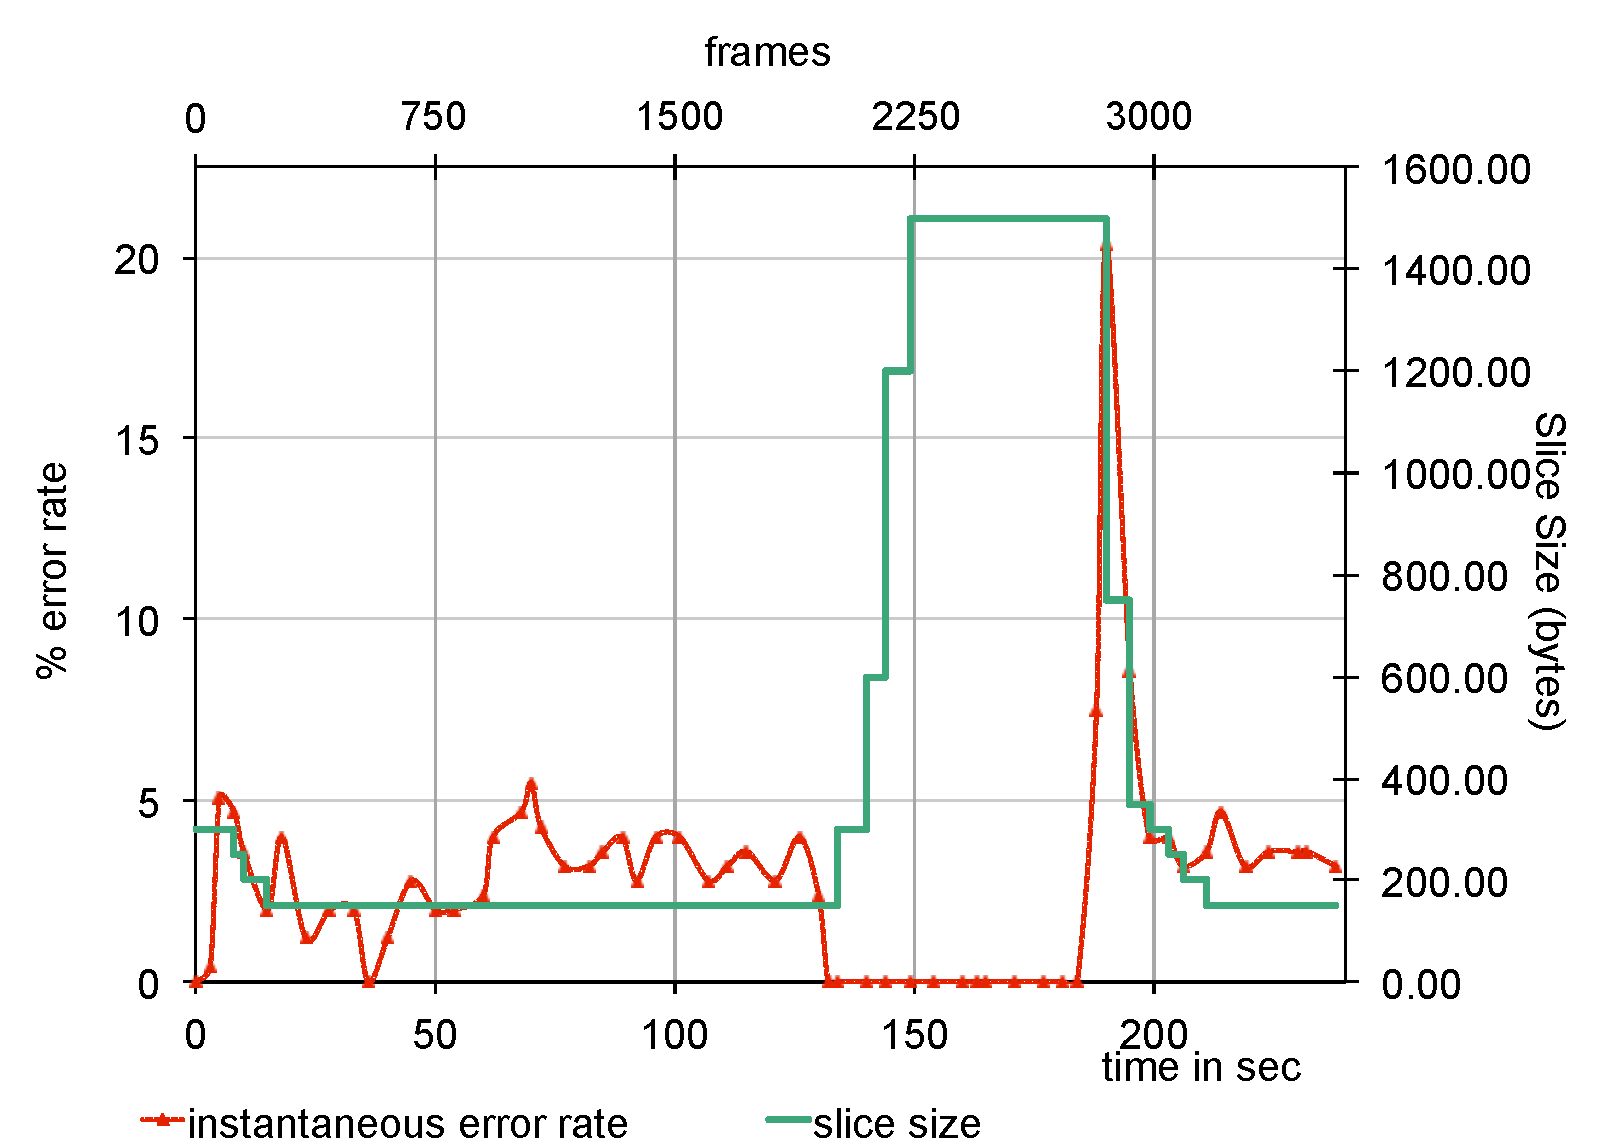
\includegraphics[width=0.66\textwidth, 
    clip=true, trim=0cm 0cm 0cm 2.5cm]{chap6-graph-ssa_adapt}
}
\caption{The plot shows the variation in slice sizes with varying error
rates.}
\label{fig:ssa_adapt}
\end{figure}

Senders use a moving average of the last three observed fraction loss rates
reported in the RTCP RR to vary the slice size. The slice size is doubled for
every period with average loss below 1.0\,\% until it reaches the MTU size
(1500 bytes). Slice sizes remain constant for loss rates between 1\,\% to
2.5\,\% to provide stability to the receiving system. However, in high loss
scenarios, if the slice size is larger than 400 bytes, it is halved, and for
sizes below 400 bytes, it is reduced in steps of 50 bytes to a minimum of 150
bytes. Figure ~\ref{fig:ssa_adapt} shows variation of slice-size with the
instantaneous loss rate and the average loss rate. Hence, by adapting the
slice sizes, the sender is not repairing the stream (or replacing the missing
packets), rather, it is attempting to constrain the area of errors in the
picture. If an RTP packet containing a small-sized slice is lost, a smaller
area of the decoded picture is affected, alternatively, when a packet
containing a large-sized slice is lost, a large part of the decoded picture 
or the complete picture is affected.

Lastly, using the RPS error-resilience mechanism, the receiver indicates the
decoding correctness when losses occur, i.e., which pictures or slices have
been decoded correctly or incorrectly.  In our experiments, the receiver sends
RTCP RR every 250\,\emph{ms}, which increases the reporting overhead to 2\,\%
of the session bandwidth. In Figure ~\ref{fig:rpsi_sim} (a), (b) and (c), we
observe that the PSNR drops down when a lost frame is referenced and the PSNR
increases immediately after the encoder chooses a correct reference picture.
When the one-way latency is 100\,\emph{ms} and the frame rate is set to 15
frames per second, we observe that the error propagation is stopped by RPS in about
4 to 7 picture frames.


\begin{figure}[!t]
  \centering{
  \subfloat [Foreman]{
    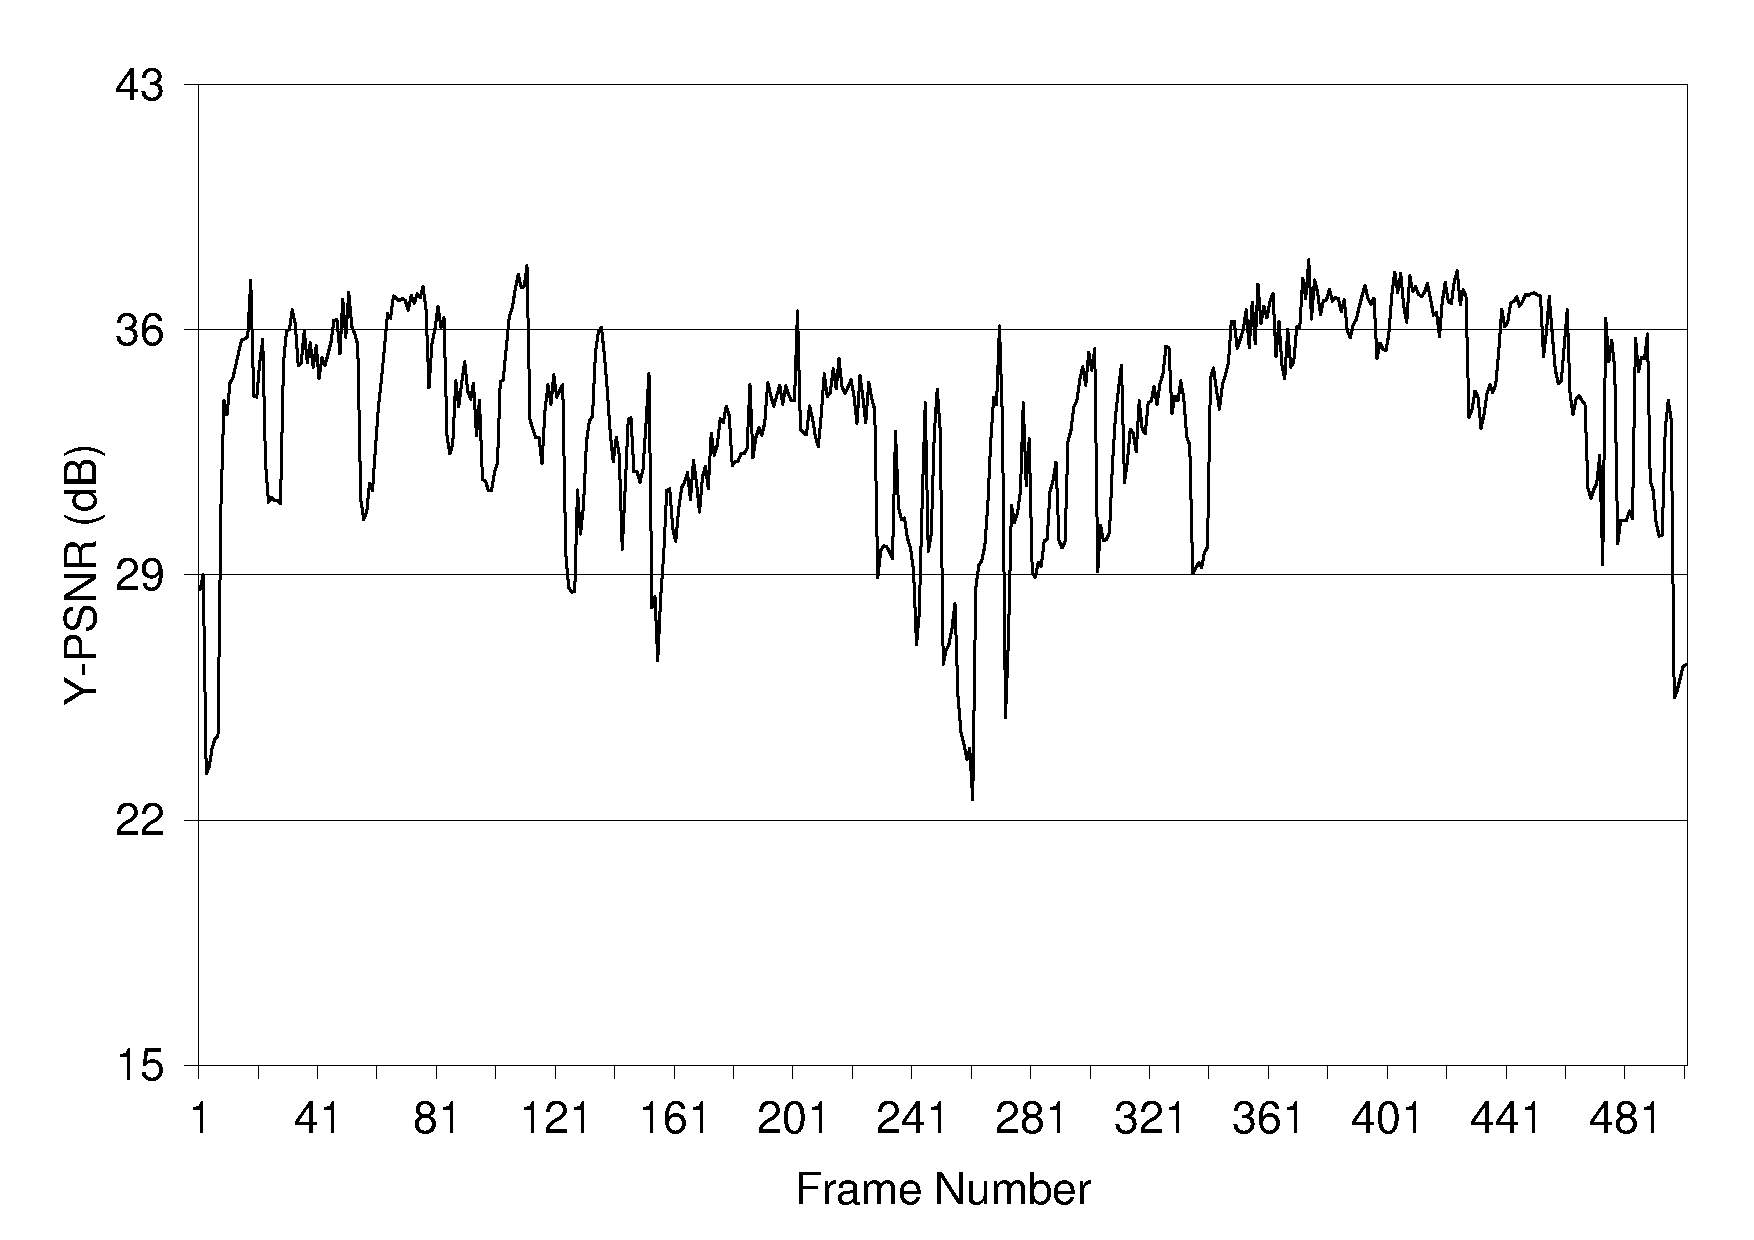
\includegraphics[width=0.5\textwidth]{chap6-graph-rpsi-1}
  }
  \subfloat [News]{
    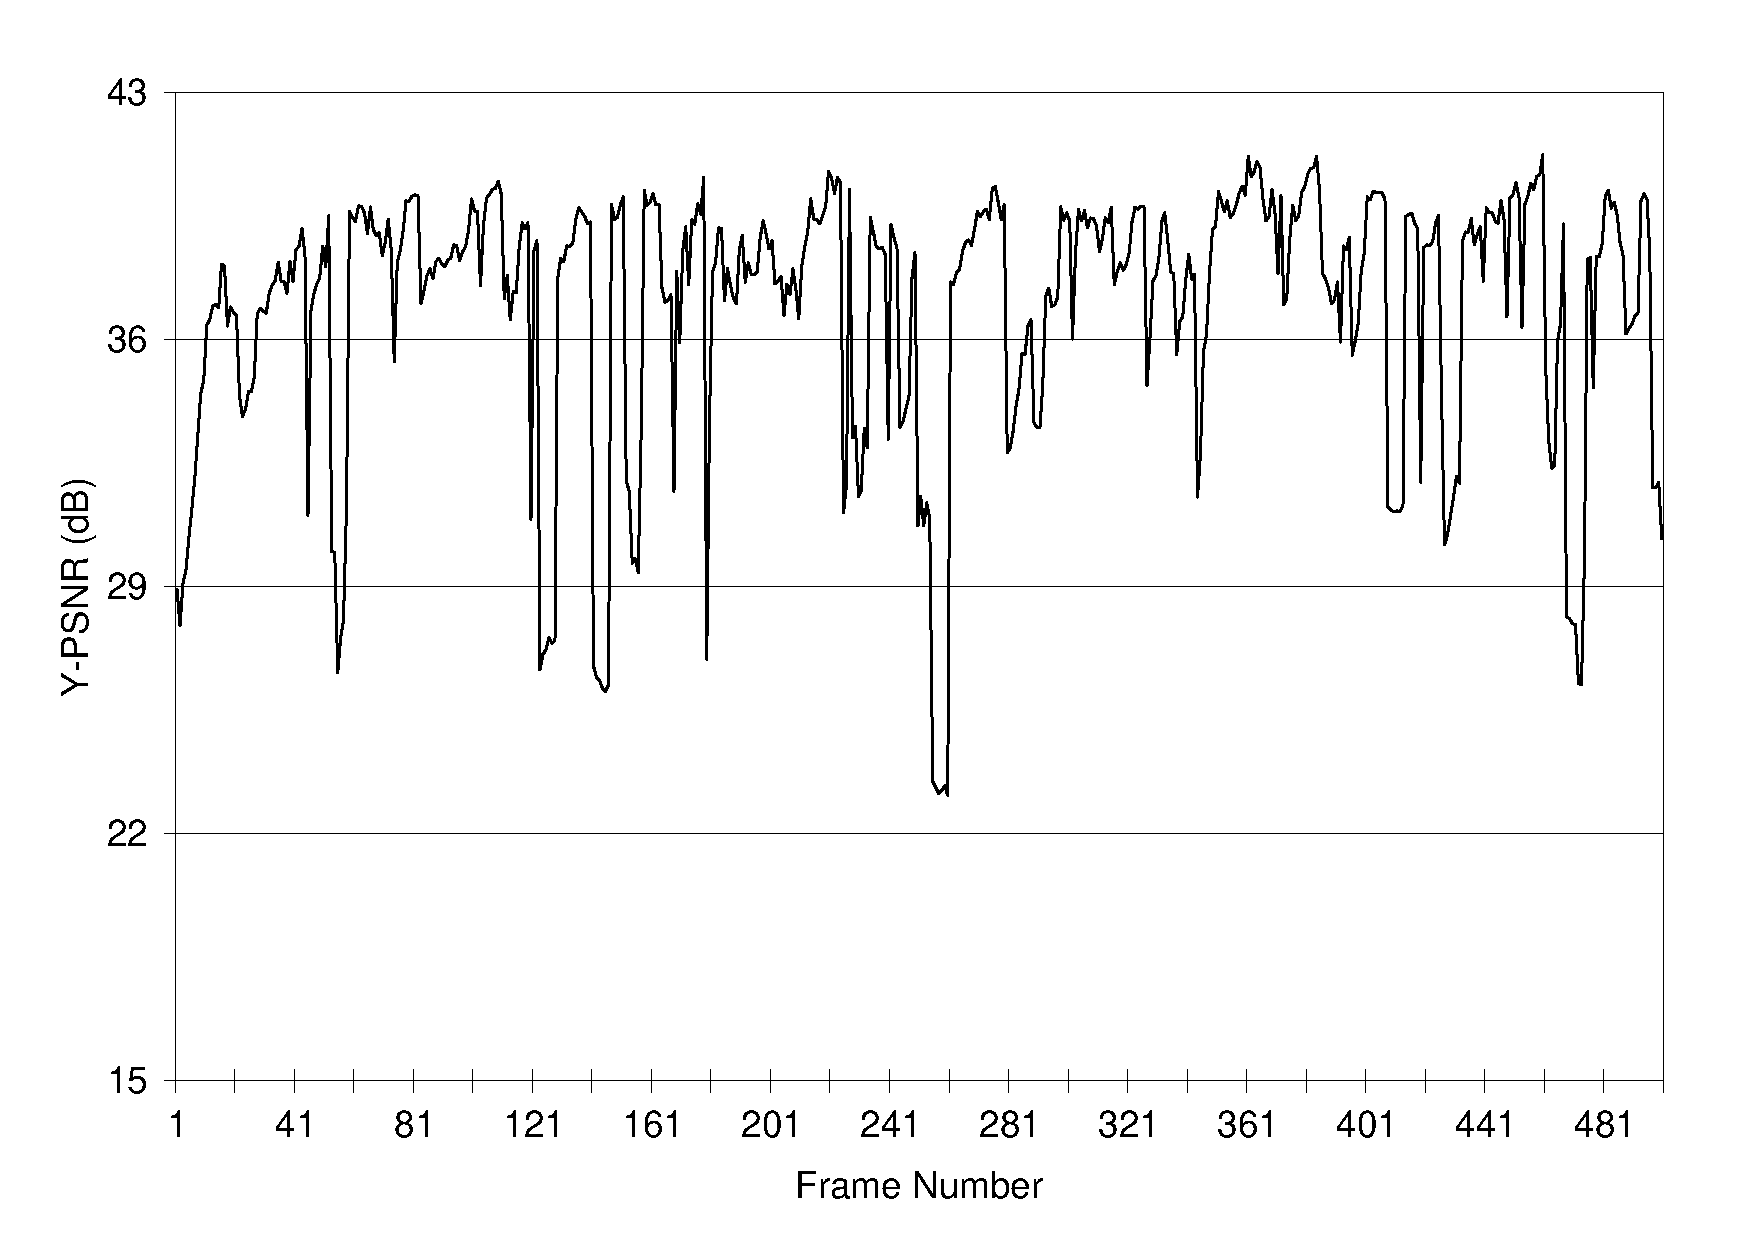
\includegraphics[width=0.5\textwidth]{chap6-graph-rpsi-3}
  } \\
  \subfloat [Football]{
    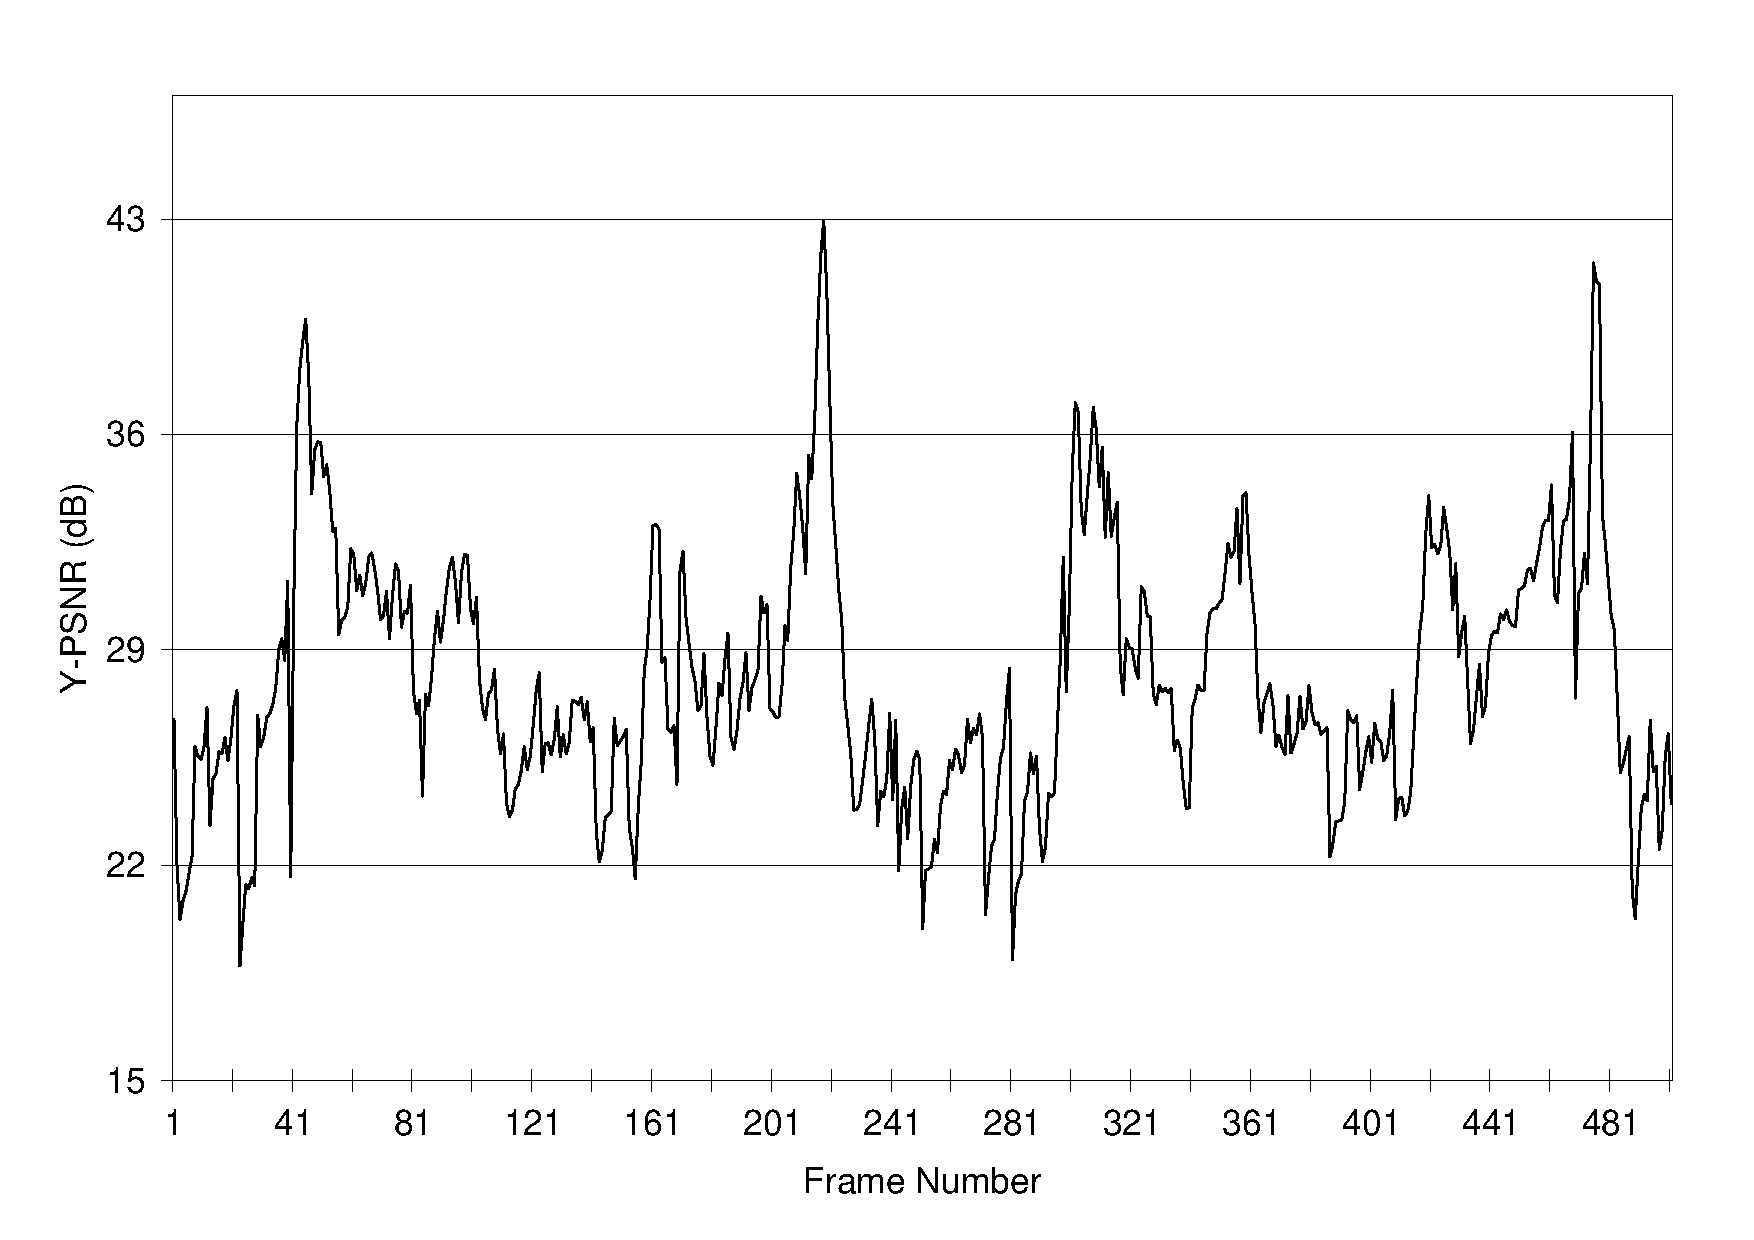
\includegraphics[width=0.5\textwidth]{chap6-graph-rpsi-5}
  }
}
\caption{The plots show the PSNR variation when using RPSI to stop decoding
error propagation for (a) Foreman, (b) News, and (c) Football sequences.}
\label{fig:rpsi_sim}
\end{figure}

Table~\ref{tab:err-sch-psnr} presents the average PSNR of the different 
error-resilience schemes for links with 0.5\,\% fractional loss. We observe that the
RPS performs better than UEP and NACK and is comparable to adaptive slices.
The UEP under performs mainly because the media stream is encoded at a lower
rate to make room for FEC, compared to the media streams of the other
error-resilience mechanisms.

\begin{table}
  \centering{
  \scalebox{0.75}{
\begin{tabular}{cccc}
\hline
 & \multicolumn{3}{l}{Y-PSNR, 0.5\,\% PLR} \\
\hline
 & Foreman & Football & News  \\ \hline
NACK & 32.1456 & 28.0331 & 35.3867 \\
RPSI & 33.68 & 28.05 & 37.37 \\
UEP & 28.33 & 26.86 & 34.47 \\
Adaptive slices & 32.30 & 28.4 & 37.25 \\
\hline
\end{tabular}
}}
\caption{Comparing the performance of different error-resilience
schemes on three different types of YUV sequences~\cite{YUV_seq}. The link
loss rate is 0.5\,\% at each 3G link.}
\label{tab:err-sch-psnr}
\end{table}

In \citepub{c:err}, we model the error-resilience mechanisms as a function of
observed packet loss and end-to-end delay (or latency), and
Figure~\ref{fig:apply_err} summarises the applicability of the
error-resilience mechanisms based on our experiments. NACK is useful when loss
rates are low and the end-to-end delay is also low. Adaptive slice size (SSA)
is applicable to the whole operational region because it attempts to scale the
packet size based on the observed loss rate, but does not help in packet
repair. RPS works better on links with bursty packet loss, where NACK would
not be effective. By correctly choosing a new reference picture, the sender is
more effective when network latency is higher. UEP/FEC schemes are mainly useful when
the sender and receiver cannot effectively co-operate to repair the stream and
the fractional loss is within the FEC's chosen protection range.

\begin{figure}
\centerline {
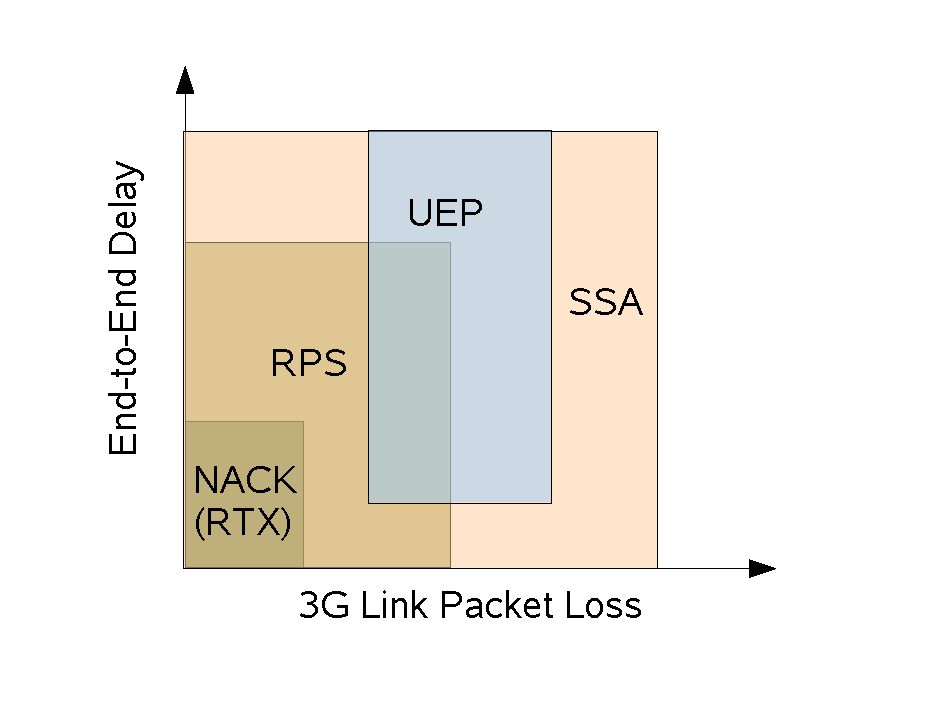
\includegraphics[width=0.75\textwidth, 
    clip=true, trim=0cm 1cm 0cm 1cm]{chap6-fig-apply-err}
}
\caption{Applicability of the error-resilience schemes in a heterogeneous
environment containing both wireless and wired links.}
\label{fig:apply_err}
\end{figure}


\section{Using FEC for Congestion Control}

For many years, conversational multimedia flows have used FEC for error 
protection~\cite{wang00review, wang98error}, i.e., the
application trades off additional sending rate for redundant packets to reduce
the effect of losses. In \citepub{c:err}, we show that 21-24\,\% of the lost
packets are recovered using a static amount of FEC. In \citepub{c:fecrc}, we
investigate the use of FEC packets not only for error-resilience but also as a
probing mechanism for congestion control.

Zhu~\textit{et al.}\cite{Zhu:2001tu,springerlink:1022865704606} propose using
ULP for both congestion control and error-resilience. 
Firstly, they estimate the available rate using a variant of TFRC,
called Multimedia Streaming TCP-Friendly Protocol (MSTFP)~\cite{871542}.
Secondly, they take packet loss and historical sending rate to smooth out the
encoding rate. Lastly, they apply FEC while performing congestion control and
their results show a significant increase in media quality. MSTFP, on the other
hand, does not use RTP/RTCP and acknowledges each packet for calculating the
TFRC estimate.

Our concept in \citepub{c:err} is similar to that described in
\cite{Zhu:2001tu} but applied to interactive multimedia. The concept is as
follows: the sender chooses a high FEC rate to aggressively probe for
available capacity and conversely chooses a low FEC rate to conservatively
probe for available capacity. While probing, if a packet is lost and the FEC
packet arrives in time for decoding, the receiver is be able to recover the
lost packet; if no packet is lost, the sender is able to increase the media
encoding rate by swapping out the FEC. Figure~\ref{fig:fecrc-intro}(a) shows
the endpoint adding FEC and then swapping it for additional media. This method
can be especially useful when the sending rate is close to the bottleneck link
rate: by choosing an appropriate FEC rate, the endpoint is able to probe for
available capacity without affecting the user-experience because the media
encoding rate remains constant.

\begin{figure}
  \centering
  \subfloat [Concept]{
    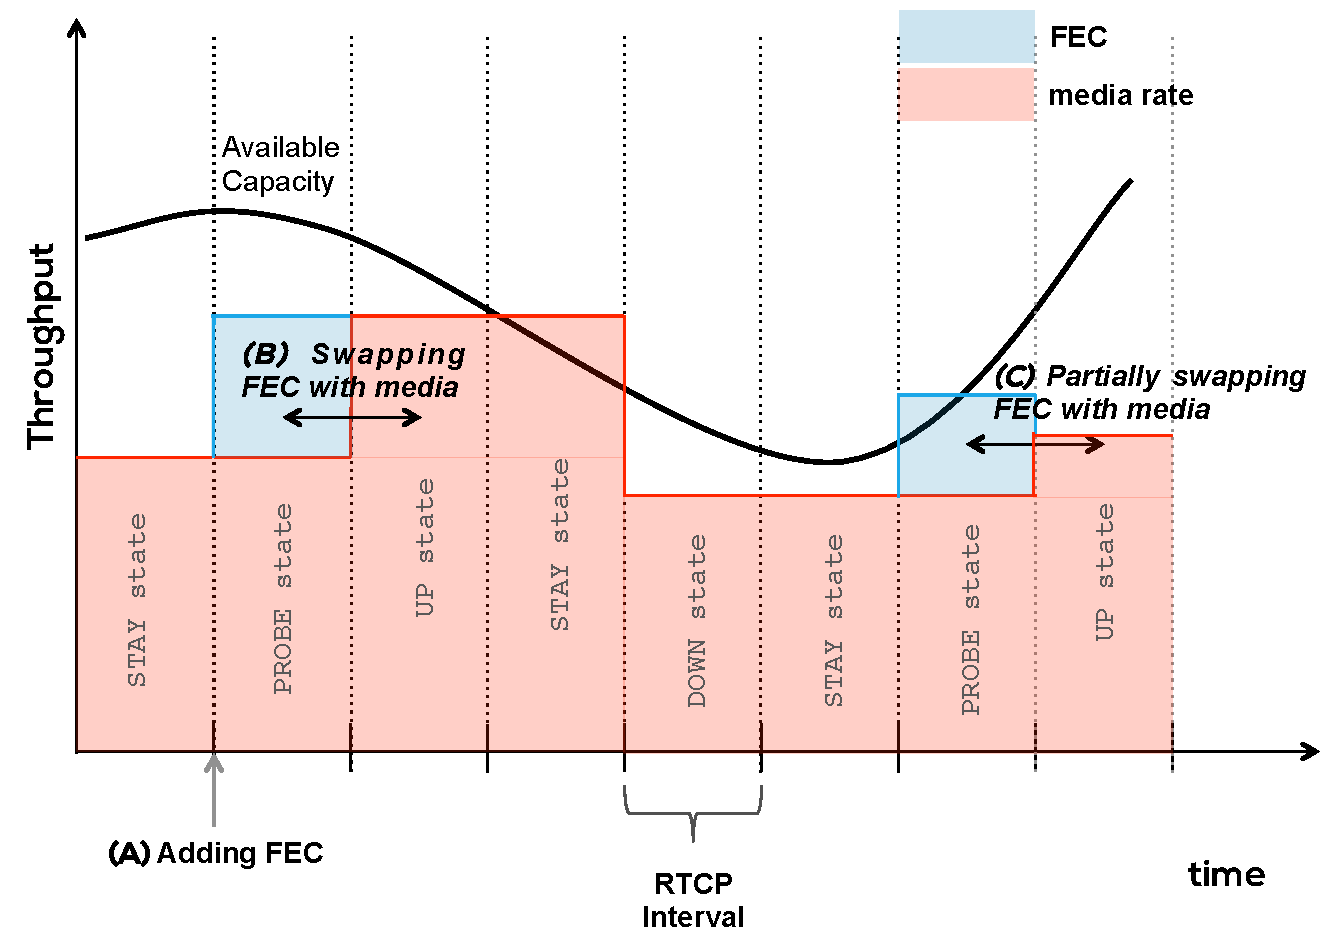
\includegraphics[width=0.66\textwidth]{chap6-fig-fecrc-concept}
  } \\
  \subfloat [State-machine]{
    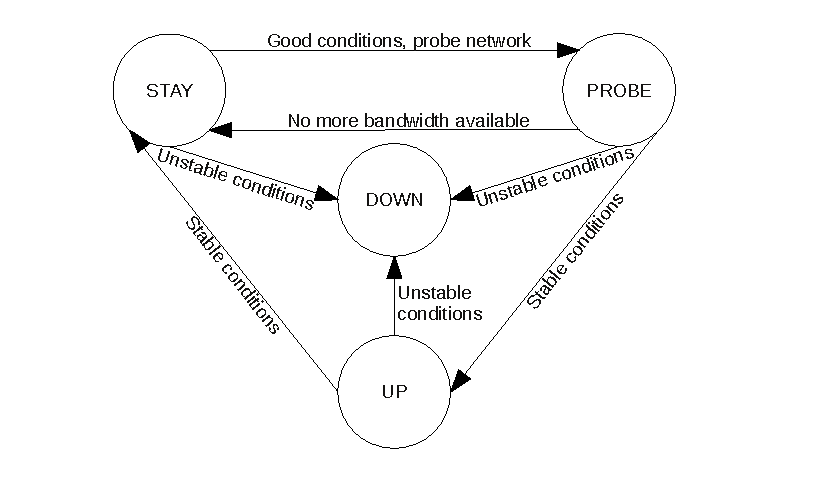
\includegraphics[width=0.66\textwidth]{chap6-fig-fecrc-state}
  }
\caption{a) Interaction of FEC and congestion control, b) FEC-Based Rate
Adaptation (FBRA) state machine.}
\label{fig:fecrc-intro}
\end{figure}

% Figure with the idea: FEC for CC

Figure~\ref{fig:fecrc-intro}(b) illustrates the state machine of a
congestion-control algorithm incorporating FEC. The state machine includes 4
states: \texttt{\textbf{STAY}}, \texttt{\textbf{PROBE}}, \texttt{\textbf{UP}},
and \texttt{\textbf{DOWN}}. The congestion control monitors the congestion
cues (such as, RTT, packet loss or discard rate~\cite{rfc7002, rfc7097, rfc7243}, jitter, frame inter-arrival
delay variation, post-repair~\cite{rfc5725, draft.xr.post.repair} etc.) to stay in the current state, or transit to
another. The state machine specifies only a generic description of path
conditions for the transition between states and leaves the interpretation to
the underlying congestion control algorithm.

After enabling FEC for an interval, one of the following three conditions may
occur: 1) No more bandwidth is available and the sender keeps the current sending
rate (\texttt{\textbf{STAY state}}), 2) Stable conditions are detected and the
sender increases the sending rate and disables FEC (\texttt{\textbf{UP
state}}), and 3) Unstable conditions are detected, and the sender reduces the
sending rate \texttt{\textbf{DOWN state}}. If FEC is disabled for the last two
intervals and no change in path characteristics is observed, FEC is enabled
(\texttt{\textbf{PROBE state}})~\cite{draft.adaptive.fec}.


\begin{figure}
  \centering{
  \subfloat [OWD=50ms]{
    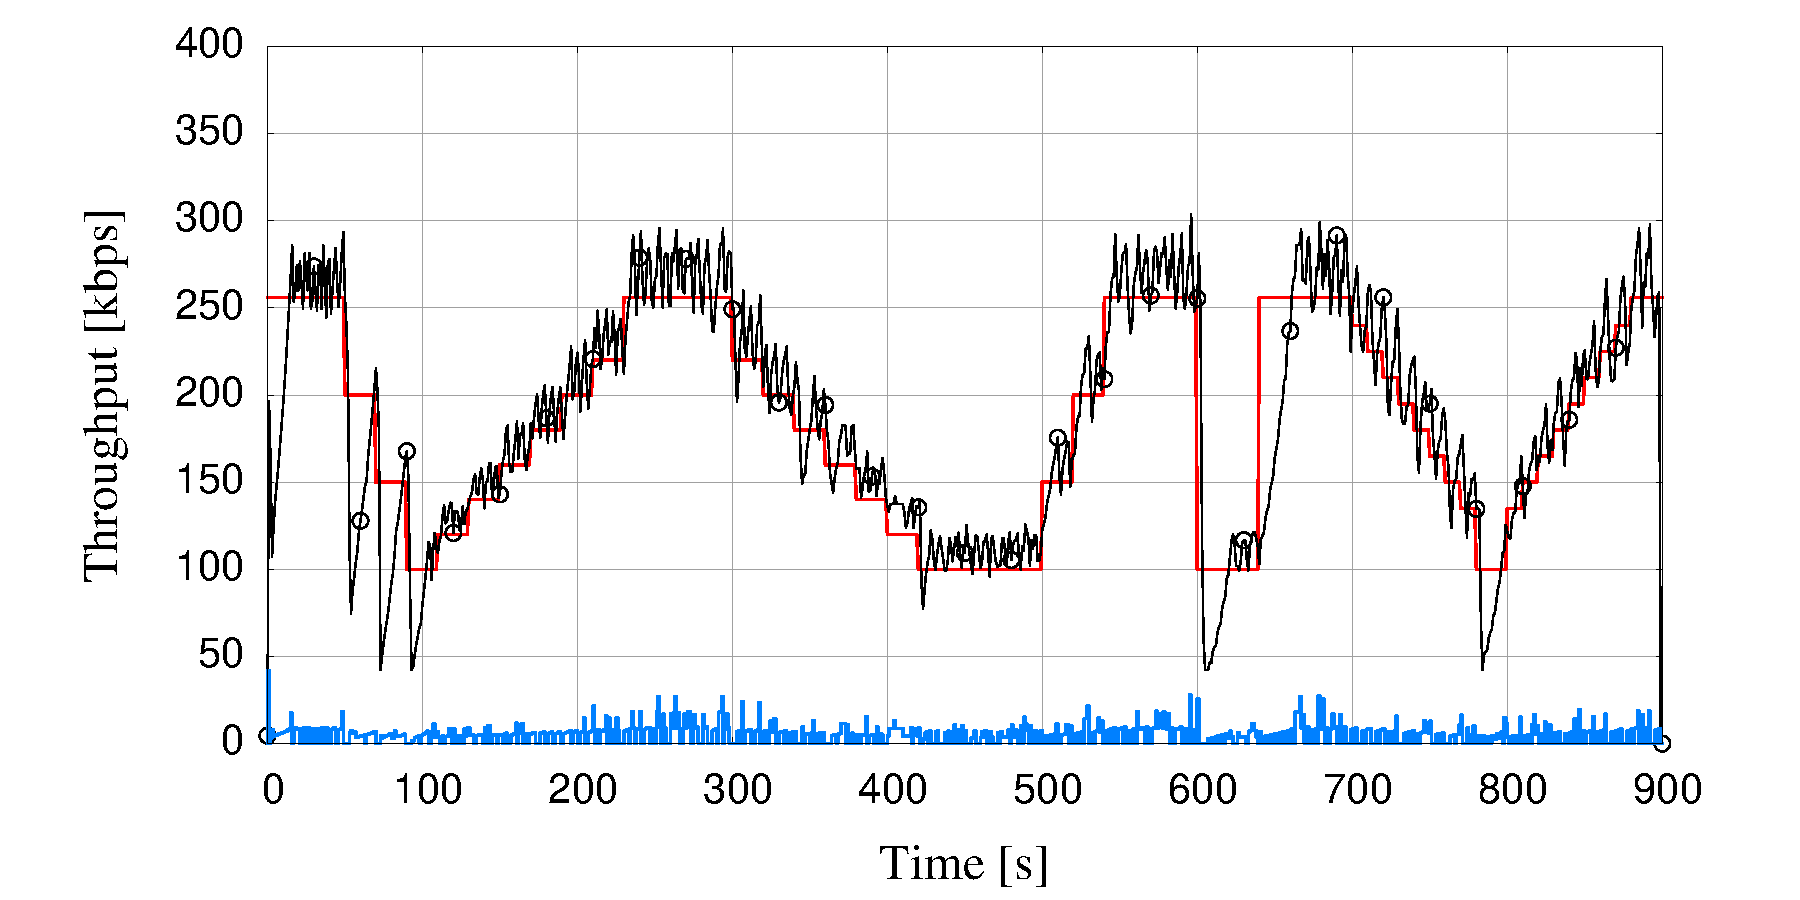
\includegraphics[width=0.5\textwidth]{chap6-graph-fecrc-var-50ms-2}
  } 
  \subfloat [OWD=100ms]{
    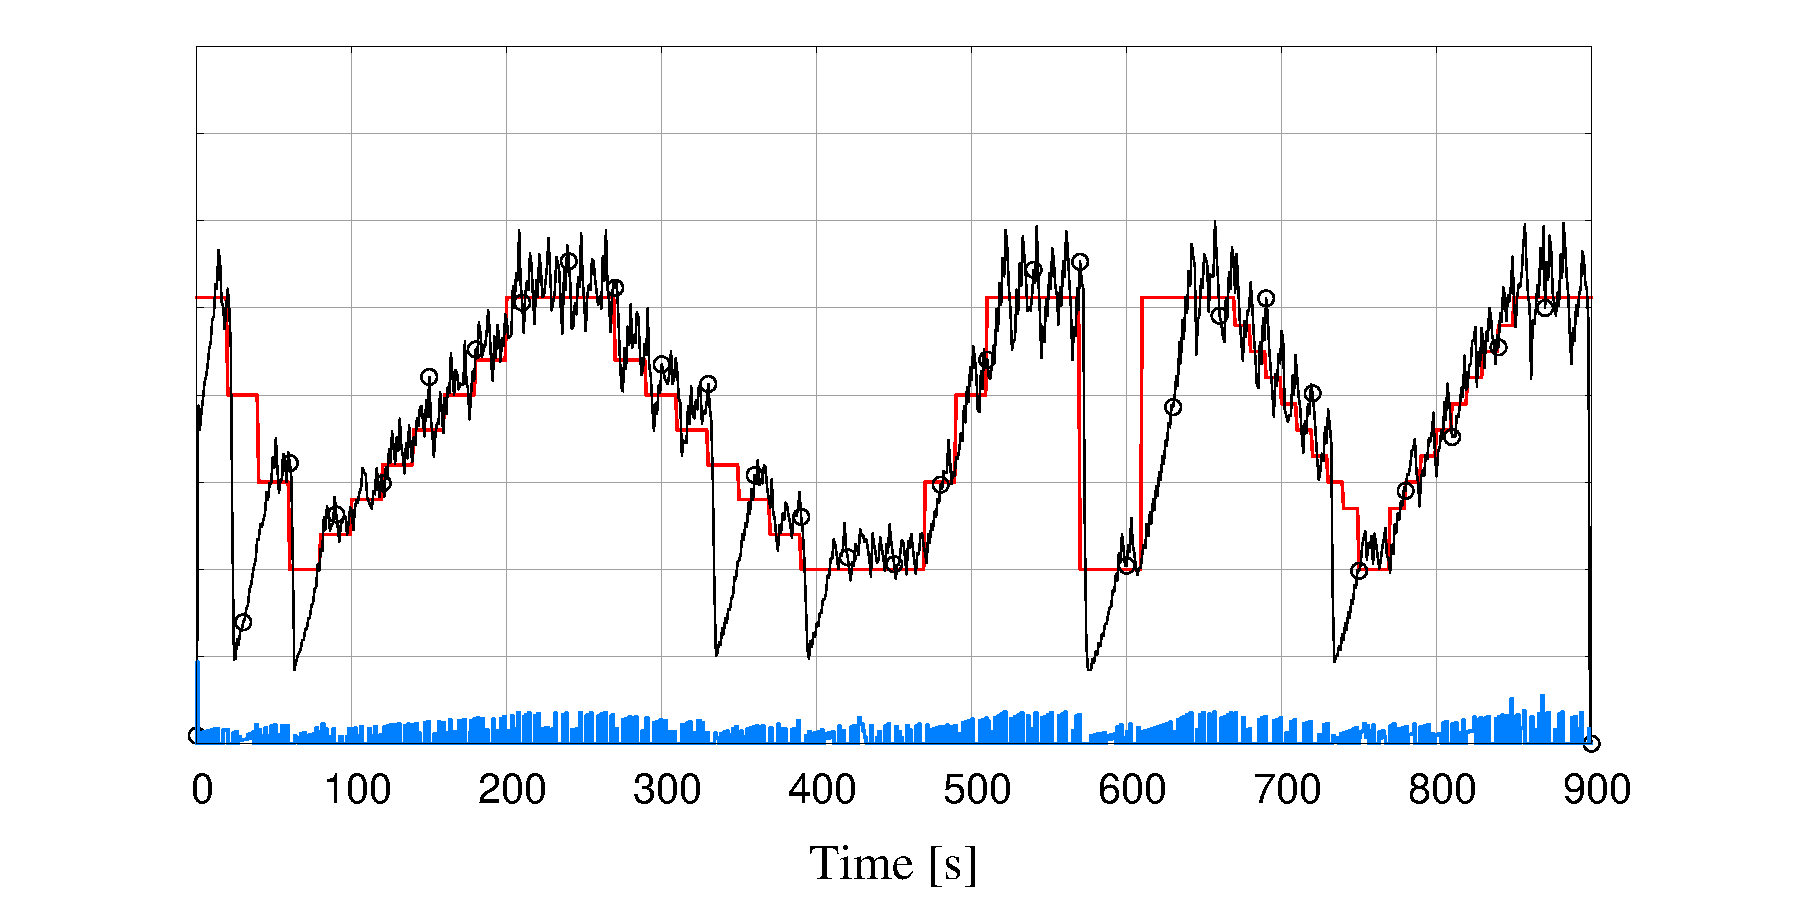
\includegraphics[width=0.5\textwidth]{chap6-graph-fecrc-var-100ms-2}
  } \\
  \subfloat [OWD = 240ms]{
    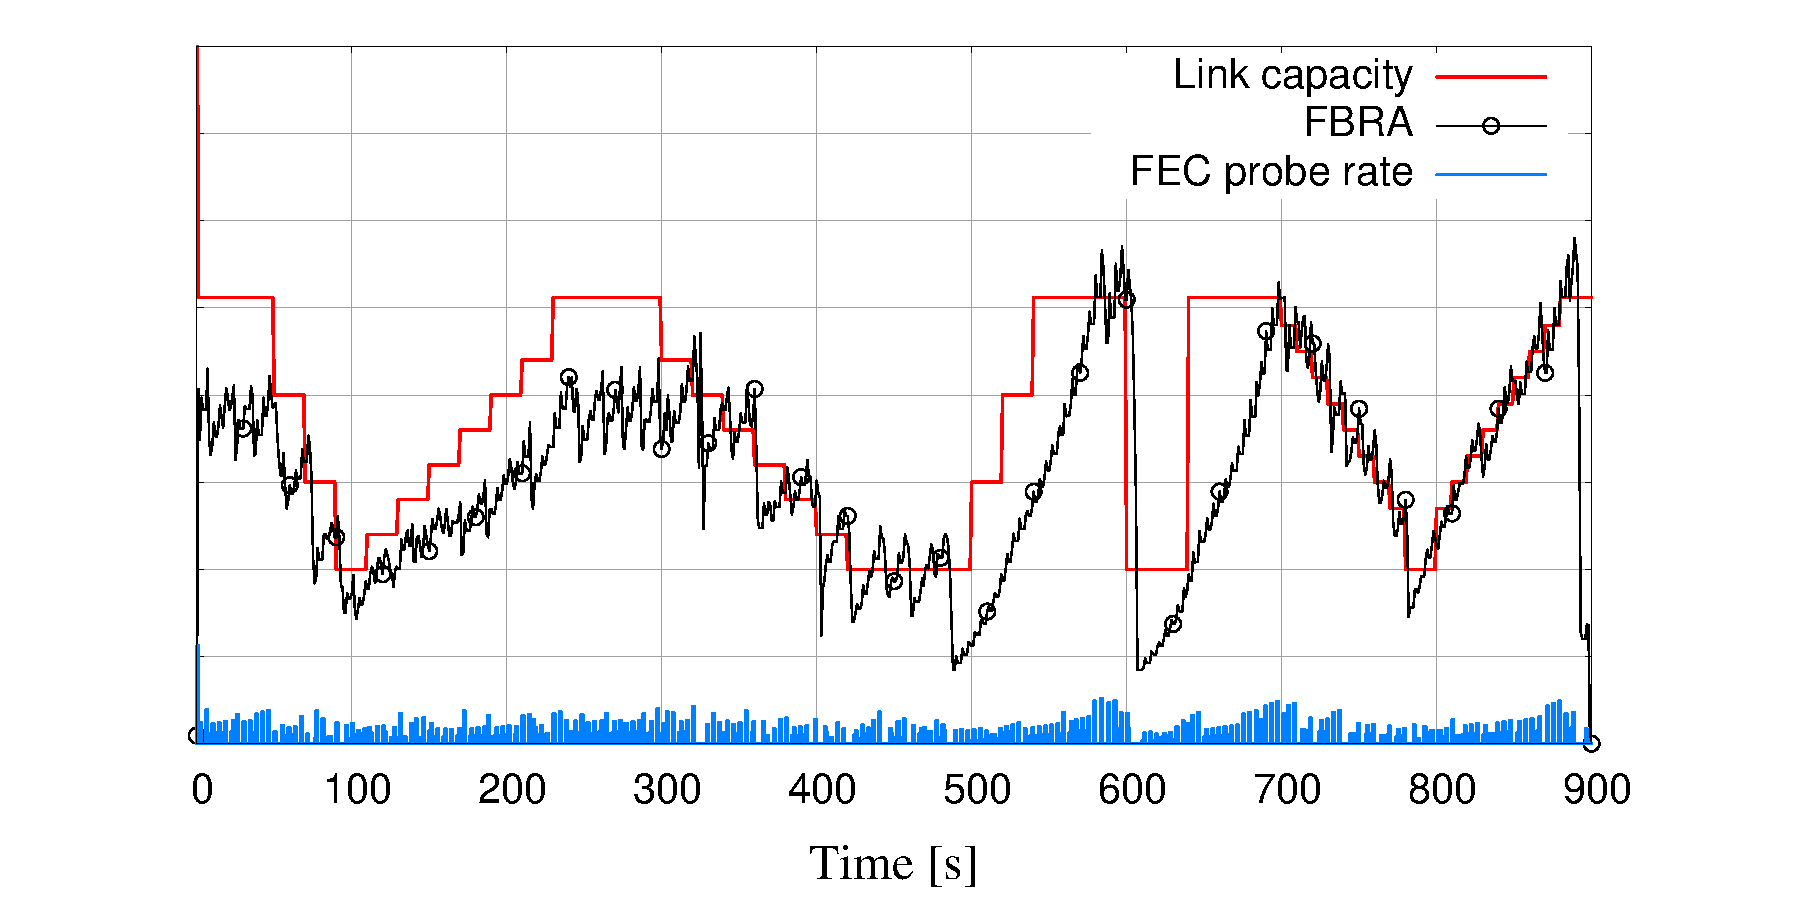
\includegraphics[width=0.5\textwidth]{chap6-graph-fecrc-var-240ms-2}
  }
}
\caption{Performance of a single RTP flow using FBRA in a
varying link capacity scenario with different bottleneck latencies. The plots
also show the FEC probing rate. We observe that the FEC rate is low when the
FBRA rate drops and FEC rate is high when the FBRA is ramping-up.}
\label{fig:fecrc-var}
\end{figure}

In \citepub{c:fecrc}, we compare the performance of FEC-Based Rate Adaptation
(FBRA), RRTCC and C-NADU. The bottleneck link capacity varies between
100\,\emph{kbps} and 256\,\emph{kbps}. In the scenario, we evaluate the
reactivity and convergence of the rate-control algorithm to the available 
end-to-end capacity for different path latencies. Our simulations in
\emph{ns-2}~\cite{ns2} shows that, for the 50\,\emph{ms} and 100\,\emph{ms}
bottleneck link latency, the goodput achieved by FBRA is comparable to RRTCC
but with comparatively lower loss rates ($\approx$1.5\,\%, see
Table~\ref{table:fecrc-var-res}). Figures~\ref{fig:fecrc-var}(a)--(b) show
that the FBRA can quite quickly bounce-back after undershooting. The figure
also shows that the FEC probing rate increases when the FBRA ramps up and the
FEC rate is low or disabled when the FBRA undershoots. However, FBRA is
primarily a delay-based control algorithm, and for the 240\,\emph{ms} bottleneck
delay, it observes that the packets are arriving very close to the 
application-defined maximum delay ($\approx$400\,ms) and is therefore, conservative in its
probing for available bandwidth (this is observed by the low FEC rate in
Figure~\ref{fig:fecrc-var}(c)). The FEC rate is about 10\,\% of the media rate at
about 15-20\,\emph{kbps} and the packet loss recovery is around 30\,\%.
Compared to FBRA, RRTCC tries to achieve high throughput at the cost of
incurring packet losses (this behaviour is also observed in \ref{tab:rrtcc-loss}), 
while C-NADU trades off packet loss for throughput. In our
experiments, FBRA's performance is placed between the two trade-offs: better
throughput than C-NADU and lower loss ratio than RRTCC.


\begin{table}
  \centering{
  \scalebox{0.75}{
  \begin{tabular}{c c c c c}
  \hline
  \multirow{2}{*}{\textbf{Delay}} & \multirow{2}{*}{\textbf{Metric}} & \textbf{FBRA} & \textbf{RRTCC} & \textbf{C-NADU} \\ \cline{3-5}
  & & avg. $\,\pm\,\sigma$ & avg. $\,\pm\,\sigma$ & avg. $\,\pm\,\sigma$ \\ \hline
  \multirow{3}{*}{\begin{sideways} 50ms \end{sideways}} & Goodput [kbps] & 179.13 $ \pm $ 2.26 &181.8 $ \pm $ 3.11& 165.42 $ \pm $ 3.87 \\ %\cline{2-8}
  & Loss rate [\%] & 1.23 $ \pm $ 0.28 & 4.27 $ \pm $ 0.78 & 0.34 $ \pm $ 0.11\\ %\cline{2-8}
  %& \textbf{FEC rate [kbps]} & 17.51 & 1.18 & - & -& -& -\\ \cline{2-8}
  & No. of lost frames & 441.43 $ \pm $ 82.37 & 1842 $ \pm $ 25.4&93.67 $ \pm $ 29.64 \\ \hline
  %& \textbf{No. of FEC protected lost frames} & 91.37 & 36.55 & - & -& -& - \\ \cline{2-8}
  %&\textbf{FRCC[\%]}& 92.57 & 2.84 & - & -& -& - \\ \hline
  \multirow{3}{*}{\begin{sideways} 100ms \end{sideways}} & Goodput [kbps] & 172.83 $ \pm $ 2.74 & 172.48 $ \pm $ 6.6 & 163.84 $ \pm $ 3.11\\ %\cline{2-8}
  & Loss rate [\%] & 1.72 $ \pm $ 0.37 & 3.09 $ \pm $ 0.85 & 0.17 $ \pm $ 0.09\\ %\cline{2-8}
  %& \textbf{FEC rate [kbps]} & 20.05 & 1.34 & - & -& -& - \\ \cline{2-8}
  & No. of lost frames & 562.83 $ \pm $ 103.44 & 740 $ \pm $ 42.82& 46.4 $ \pm $ 22.94\\ \hline
  %& \textbf{No. of FEC protected lost frames} & 130.57 & 45.41 & - & -& -& - \\ \cline{2-8}
  %& \textbf{FRCC[\%]} & 95.85 & 1.95 & - & -& -& - \\ \hline
  \multirow{3}{*}{\begin{sideways} 240ms \end{sideways}} &Goodput [kbps] & 144.89 $ \pm $ 8.35 & 169.22 $ \pm $ 5.68 & 153.52 $ \pm $ 6.81\\ %\cline{2-8}
  & Loss rate [\%] & 2.82 $ \pm $ 0.89 & 2.98 $ \pm $ 0.55&0.19 $ \pm $ 0.07 \\ %\cline{2-8}
  %& \textbf{FEC rate [kbps]} & 16.22 & 0.56 & - & -& -& - \\ \cline{2-8}
  & No. of lost frames & 789.93 $ \pm $ 223.55 & 705.67 $ \pm $ 41.33 & 53.23  $ \pm $ 21.41 \\ \hline
  %& \textbf{No. of FEC protected lost frames} & 178.07 & 69.92 & - & -& -& - \\ \cline{2-8}
  %& \textbf{FRCC[\%]} & 90.1 & 7.26 & - & -& -& - \\ \hline
  \end{tabular}
  }}
  \caption{Overall metrics for an RTP flow on a variable capacity link.
  Results are the average of 30 runs.}
  \label{table:fecrc-var-res}
\end{table}


% RRTCC achieves the best goodput ($169$-$180 kbps$) for the three bottleneck
% link latencies, but has the worst loss rate ($3$-$4\%$). RRTCC is aggressive
% in its probing for available bandwidth and does not react to losses up to
% $2\%$. On the other hand, C-NADU achieves excellent reliability
% ($0.15$-$0.5\%$) results in all the cases, but observes lower goodput (about
% $10$-$15\,kbps$ lower than RRTCC). The two algorithms trade-off throughput for
% packet loss and vice-versa.

% Table of FEC, C-NADU and RRTCC :)


\begin{table}
  % \resizebox{\textwidth}{!}{%
  \centering{
  \scalebox{0.75}{
  \begin{tabular}{cccc}
  \hline
  \multirow{2}{*}{\textbf{Delay}} & \multirow{2}{*}{\textbf{Metric}} & \textbf{Call 1} & \textbf{Call 2} \\ \cline{3-4}
  & & avg. $ \pm \sigma$ & avg. $ \pm \sigma$ \\ \hline 
  \multirow{5}{*}{\begin{sideways} 50ms \end{sideways}} 
  & Goodput [kbps] & 375.39 $ \pm $ 88.25 & 348.77 $ \pm $ 83.64 \\ 
  & Loss rate [\%] & 1.21 $ \pm $ 0.19 & 1.39 $ \pm $ 0.69 \\ 
  & FEC rate [kbps] & 12.24 $ \pm $ 1.64 & 11.78 $ \pm $ 1.39 \\ 
  & No. of FEC protected lost frames & 15.3 $ \pm $ 3.44 & 14.6 $ \pm $ 2.73 \\ 
  & No. of recovered frames & 7.4 $ \pm $ 2.83 & 6.9 $ \pm $ 3.33 \\ 
  & PSNR [dB] & 38.08 $ \pm $ 2.1 & 37.7 $ \pm $ 1.53 \\ \hline
  %& \textbf{Lossless PSNR [dB]} &  &  &  &  \\ \hline 
  \multirow{5}{*}{\begin{sideways} 100ms \end{sideways}} 
  & Goodput [kbps] & 295.33 $ \pm $ 48.27 & 351.1 $ \pm $ 63.4 \\ 
  & Loss rate [\%] & 3.15 $ \pm $ 0.93 & 2.33 $ \pm $ 0.87 \\ 
  & FEC rate [kbps] & 10.7 $ \pm $ 0.68 & 11.69 $ \pm $ 1.52 \\ 
  & No. of FEC protected lost frames & 3.0 $ \pm $ 2.1 & 4.1 $ \pm $ 3.14 \\ 
  & No. of recovered frames & 7.3 $ \pm $ 3.03 & 4.5 $ \pm $ 3.07 \\ 
  & PSNR [dB] & 35.64 $ \pm $ 1.17 & 37.32 $ \pm $ 1.65 \\ \hline
  %& \textbf{Lossless PSNR [dB]} & & & & \\ \hline 
  \end{tabular}
  }}
  \caption{Two FBRA flows on a bottleneck link in an emulated testbed. Results
  are the average of 10 runs.}
  \label{table:fecrc-rw-udp}
\end{table}

In \citepub{c:fecrc}, we also measure the performance of two FBRA calls
competing on a bottleneck link (1\,\emph{Mbps}) in a testbed. The difference in the
goodput of the calls in the two latency scenarios (50\,\emph{ms} and
100\,\emph{ms}) is about 30-50\,\emph{kbps}, but the PSNR of these calls is
similar (see Table~\ref{table:fecrc-rw-udp}). Therefore, as far as we can tell from
PSNR, the small rate variations have little bearing on the quality of the
call. The FEC recovery is low due to the small amount of packet loss, and most of
the losses occur when FEC was disabled. Additionally, 90\,\% of the times FEC
was enabled resulted in an increase in media rate. Low FEC overhead also
implies that the FBRA remains longer in the \texttt{\emph{STAY}} state, thus
avoiding abrupt changes to the encoding rate, which is detrimental for user
experience \cite{Zink03subjectiveimpression}.

\begin{table}
  % \resizebox{\textwidth}{!}{%
  \centering{
  \scalebox{0.75}{
  \begin{tabular}{ccc}
  \hline
  \textbf{Metric} & \textbf{50ms delay} & \textbf{100ms delay} \\ \cline{2-3}
  & avg. $ \pm \,\sigma$ & avg. $ \pm \,\sigma$ \\ \hline 
  Goodput [kbps] & 302.24 $ \pm $ 87.07 & 280.97 $ \pm $ 92.15 \\
  Loss rate [\%] & 4.24 $ \pm $ 0.89 & 4.1 $ \pm $ 0.58 \\
  FEC rate [kbps] & 13.6 $ \pm $ 2.15 & 12.58 $ \pm $ 2.18 \\
  No. of lost frames & 154.6 $ \pm $ 16.56 & 170.9 $ \pm $ 12.38 \\
  No. of FEC protected lost frames & 38.0 $ \pm $ 6.08 & 23.7 $ \pm $ 8.99 \\ 
  No. of recovered frames & 7.4 $ \pm $ 2.83 & 6.9 $ \pm $ 3.33 \\
  PSNR [dB] & 35.62 $ \pm $ 1.49 & 34.7 $ \pm $ 2.26 \\
  TCP throughput [kbps] & 612.22 $ \pm $ 48.45 & 575.11 $ \pm $ 45.67 \\ \hline
  %\textbf{Lossless PSNR [dB]} &  &  &  &  \\ \hline 
  \end{tabular}
  }}
  \caption{An RTP flow sharing a bottleneck link with short TCP flows in an
  emulated testbed. Results are average of 10 runs.}
  \label{table:fecrc-rw-tcp}
\end{table}


When competing with short TCP flows, the FBRA achieves an average goodput of
302\,\emph{kbps} and 280\,\emph{kbps} in the 50\,\emph{ms} and 100\,\emph{ms}
latency scenario, respectively (see Table~\ref{table:fecrc-rw-tcp}).
Additionally, about 85\,\% of the times FEC was enabled, resulted in an
increase in media rate. The TCP flow achieves a throughput of around
600\,\emph{kbps} on average. The PSNR in both scenarios are very similar
($\approx$ 35dB), but the PSNR is lower for the 100\,\emph{ms} delay scenario because the
average goodput is also a bit lower in this case (see Figure~\ref{fig:fecrc-dnet}).


\begin{figure}
  \centering{
  \subfloat [50ms]{
    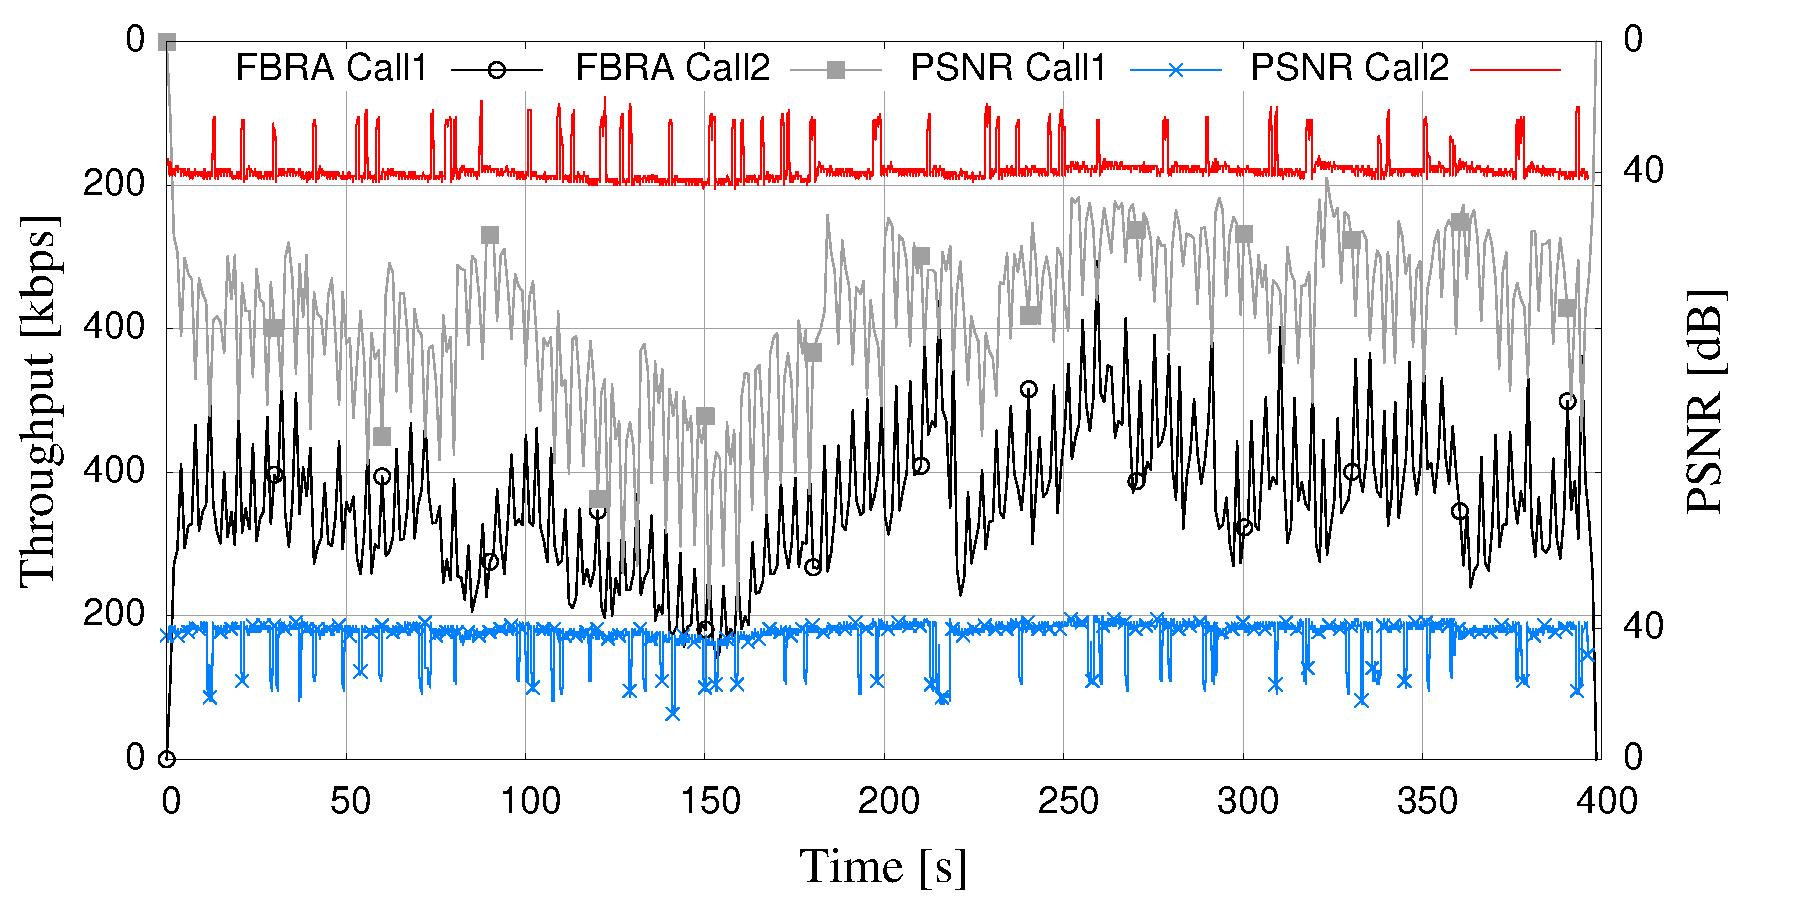
\includegraphics[width=0.66\textwidth]{chap6-graph-fecrc-dummynet-50ms-2}
  } \\
  \subfloat [100ms]{
    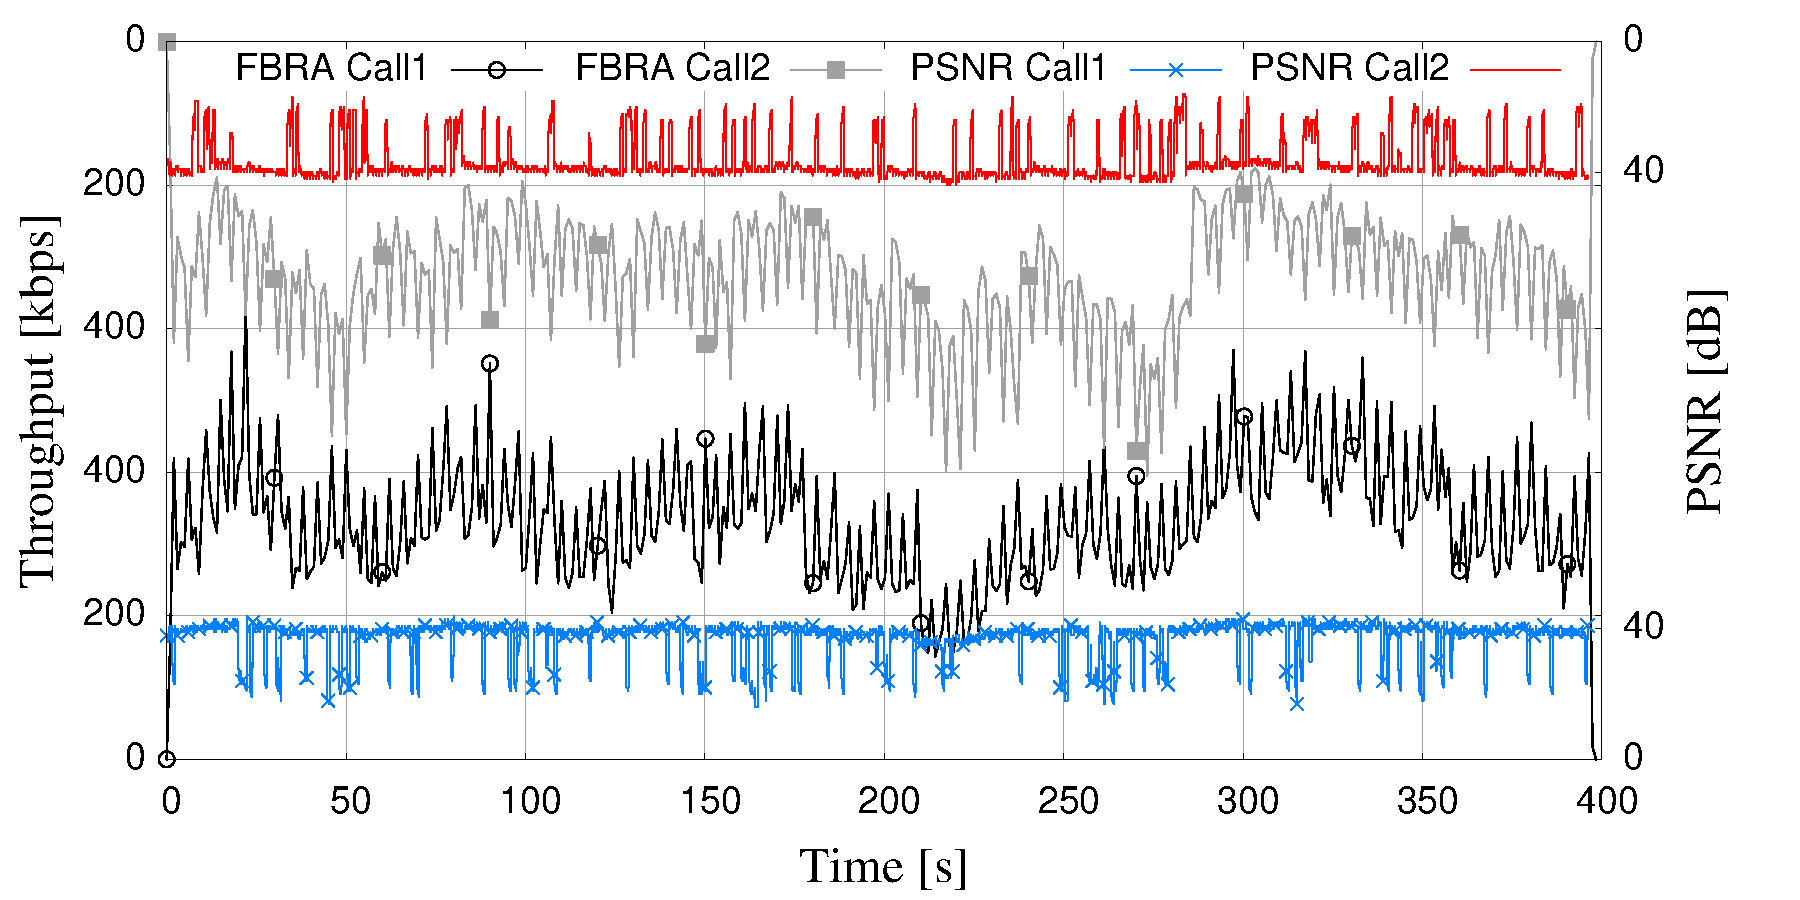
\includegraphics[width=0.66\textwidth]{chap6-graph-fecrc-dummynet-100ms-2}
  }
}
\caption{The plots show the goodput of two RTP calls sharing a common
bottleneck. To illustrate amount of empty link capacity and how two flows push
one another, we plot one of them on the reverse axis. The end-to-end path
capacity is 1\,\emph{Mbps} in both delay scenarios and delays are 50\,\emph{ms}
and \emph{100ms}. The plot also shows the PSNR variation for the two calls (on
the minor Y-axis).}
\label{fig:fecrc-dnet}
\end{figure}

% Lastly, we measure the performance of the FBRA on the public Internet, between
% a host on Amazon EC2 instance in Ireland and a machine at Aalto University. We
% observe varying results between each successive run, as the public Internet
% has varying amount of cross traffic. The goodput ranges between $100$-$700$
% \emph{kbps}, the maximum loss rate does not exceed $1.5\%$, the PSNR of the
% calls varies between $35$-$40$ \emph{dB}. Despite the diversity in results, it
% show that FBRA may work in the public Internet.

\section{Summary}

In this chapter, we address two problems: applicability of error-resilience
schemes and the use of FEC to probe for available capacity in a multimedia congestion
control algorithm. In the first case, we show that NACK, RPS, UEP/FEC and adaptive 
slice-size can be used for different levels of latencies and observed packet
loss ratio. We also observed that sending smaller packets in mobile networks
performed better than sending MTU-sized ($\approx$ 1500 bytes) packets.
Alternatively, the MTU sized packets were better suited for wired or fixed
networks where bit errors occurred less often.

In the second case, we propose a congestion control scheme where instead of
increasing the rate when network conditions seem stable, the sender introduces
FEC for one RTCP interval. If the FEC and the media packets are received
successfully, sender rate increases by the amount of the FEC rate. 
The trade-off is that we get a smoother ramp-up and, if a packet gets
lost, it may be recovered by the FEC packet. The sender also implements a
variable FEC interval, i.e., it varies the number of packets for which FEC is
generated. Hence, if the sender thinks that it is under utilising the link by a
large margin, it introduces a shorter FEC interval (up to 33\,\% redundancy)
and therefore ramps up quickly. Consequently, when the sender thinks that it is closer
to the bottleneck link capacity, it introduces a longer FEC interval (up to
8\,\% redundancy) and therefore is conservative in probing for available
capacity. Our experiments show that by using adaptive FEC for probing, the
endpoints are able to recover 15-25\,\% of the lost packets, and,
$\approx$90\,\% of the time, using FEC subsequently results in an increase in
the media rate. These results are comparable to our earlier experiments using
a fixed FEC interval for error-resilience, where we were able to recover
20-24\;\% of the lost packets. We believe using FEC for congestion control in
interactive multimedia has not been explored in depth by the community, partly
because interactive multimedia flows have very tight delay constraints and FEC
may not arrive in time for recovering the packet.

This chapter concludes the discussion of congestion control based on 
\emph{in-path} sources and \emph{in-band} signalling. In the next two chapters, we will
discuss the use of congestion cues from off-path sources to perform congestion
control.


\chapter{Mobility, Offloading, Multihoming, and Overlays}
\label{chap:mprtp}
Figure~\ref{fig:4:fw} in Chapter~\ref{chap:cc.fw} shows the structure of the
congestion control framework described in this thesis. The framework
categorizes \emph{Out-of-path} sources and \emph{in-band} signaling for
implementing congestion control (corresponds to \emph{Block C} in
Figure~\ref{fig:4:fw}), which are discussed in this chapter. This chapter is
based on our work on Multipath RTP (MPRTP), which is documented in
\citepub{c:mprtp}, in \cite{draft.mprtp}, \cite{draft.mprtp.sdp},
\cite{Globisch:AsymGrpComm}, and \cite{draft.rtcp.overlay}.

In \citepub{c:mprtp}, we propose the following: design goals of implement a
multipath protocol for multimedia, protocol details, scheduling algorithm to
send media packets over multiple paths, a dejitter buffer implementation to
playout packets smoothly even when the path skew is high. We evaluate the
performance of the proposed mechanisms in diverse scenarios in our testbed.
Lastly, we discuss the system consideration for deployment. 

In \cite{draft.mprtp}, we describe the requirements, functional blocks and
protocol formats to extend RTP for enabling multipath capabilities. However,
this document does not define a scheduling algorithm and allows for multiple
proposals. In \cite{draft.mprtp.sdp}, we describe SDP and RTSP extensions
required to setup MPRTP sessions and also ICE extensions to advertise MPRTP
interfaces and perform NAT traversal.

In \cite{Globisch:AsymGrpComm}, we propose using a network topology with
multiple distribution trees to distribute video streams in a very large call
video conference with few active speakers and many passive participants
listening in. The multiple distribution trees carry separate MPRTP subflows
and participants are members of multiple distribution trees, but actively
forward media flows in one of the distribution trees. Therefore, a node is an
overlay node in a few (e.g., one) distribution trees and a leaf node in the
rest. In the paper, we use a centralized focus to manage the joining, leaving
and inserting the participant in the appropriate position in the distribution
tree. \cite{draft.rtcp.overlay} is a work in progress and proposes protocol
extensions to perform tree constructions in a distribution tree without the
need of a centralized conferencing focus.


\section{Multipath RTP (MPRTP)}

The Internet backbone has evolved over the past decades to a mesh of service
providers with manifold peerings that are generally capable of offering a
number of (independent) paths between two nodes. Networks often use multiple
attachment points for resilience purposes, such as data enterprise networks or
data centers and even routers for SOHO networks support multiple access
networks~\cite{draft.fun.multi, draft.homenet.arch}. Additionally, many hosts
today feature multiple network interfaces (e.g., WLAN and 3G on mobile
devices), this may yield the possibility for two endpoints to communicate via
multiple paths. While exploiting multipath characteristics
\cite{Wischik:2008:RPP} has been explored for TCP (e.g.,
MPTCP~\cite{rfc6824}), the requirements for real-time traffic differs notably
and TCP can at best serve real-time communication within tight delay
constraints of the network~\cite{Brosh:tcp-real-time}. In the multipath case,
the scheduling algorithms do not consider real-time bounds when spreading data
segments across different paths and diverse paths may lead to worst case delay
and thus even longer buffering time.

\begin{figure}
\centerline {
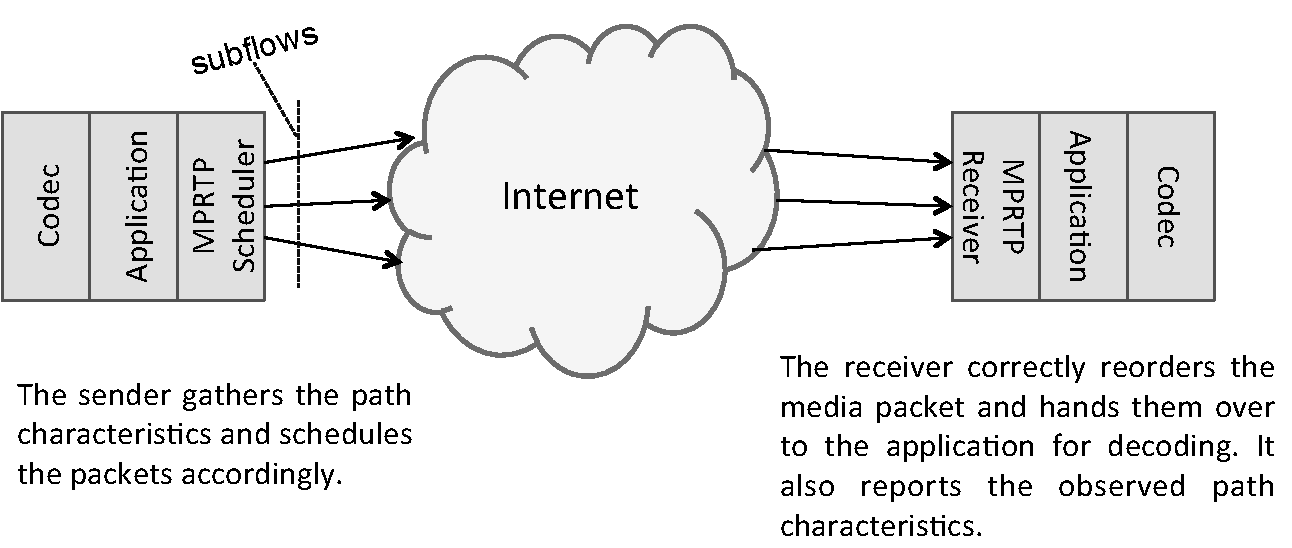
\includegraphics[width=0.9\textwidth]{chap7-fig_mprtp-1}
}
\caption{System Overview: A sender uses multiple paths to stream media
  to a receiver.  The receiver uses a dejitter buffer to reorder
  packets and sends per-path characteristics to the sender that
  distributes the packets based on the reported values.}
\label{chap7:fig_mprtp}
\end{figure}

We propose Multipath RTP (MPRTP) as a backwards compatible extension to
RTP~\cite{rfc3550}, it is documented in \cite{draft.mprtp} and defines the
basic mechanisms to operate across multiple parallel paths.
Figure~\ref{chap7:fig_mprtp} shows a macroscopic system overview of MPRTP. The
primary use-case for MPRTP is transporting media flows between multi-homed
endpoints. Such endpoints could be residential IPTV or telepresence devices
that connect to the Internet through two different Internet service providers
(ISPs), or mobile devices that connect to the Internet through 3G and WLAN
interfaces. By allowing RTP to use multiple paths for transmission, the
following gains can be achieved:

\begin{enumerate}
\setlength{\itemsep}{5pt}

\item \textbf{\texttt{Higher quality}}: Pooling the resource capacity of
multiple Internet paths allows higher bit-rate and higher quality codecs to be
used. From the application perspective, the available bandwidth between the
two endpoints increases.

\item \textbf{\texttt{Load balancing}}: Transmitting an RTP stream over
multiple paths reduces the bandwidth usage on a single path, which in turn
reduces the impact of the media stream on other traffic on that path. Also by
seamlessly offloading a flow from one path to another allows for some gains,
for example, reduces energy consumption, reduces access costs, or reduces
network latency.

\item \textbf{\texttt{Fault tolerance}}: Using multiple paths in conjunction
with redundancy mechanisms (FEC, re-transmissions, etc.), outages on one path
have less impact on the overall perceived quality of the stream. This can also
enable seamless handover in the case of mobility, i.e., moving from one
network to another.

\end{enumerate}


\begin{figure}
\centerline {
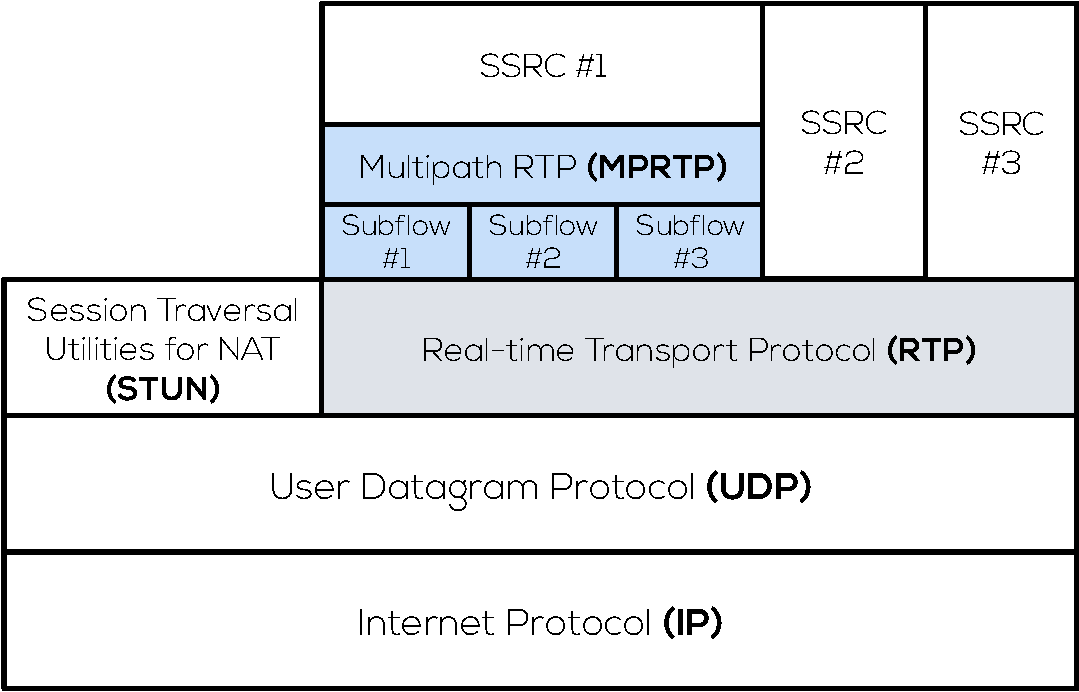
\includegraphics[width=0.75\textwidth]{chap7-fig-mprtp-stack}
}
\caption{The RTP and MPRTP stack working alongside each other. SSRC $\#1$ uses
MPRTP while SSRC $\#2$ and SSRC $\#3$ uses single path RTP.}
\label{chap7:fig_mprtp_arch}
\end{figure}

Figure~\ref{chap7:fig_mprtp_arch} compares the network stack of a single path
and a multipath-capable endpoints. SSRC \#2 and SSRC \#3 use a single path,
while SSRC \#1 uses multiple paths (with two subflows for the two interfaces).
Subflow \#1 and \#2 are expected flow over IP address \#1 and \#2,
respectively. To discover its multiple interfaces, the multimedia application
either uses the ICE procedures (hence, STUN) or polls the kernel repeatedly.

The design goals for MPRTP from our perspective are: MPRTP-enabled system to
be able to make use of multiple paths and adapt to their relative capacity
changes by redistributing the load. As different paths will likely exhibit
different RTTs, mechanisms must be developed to overcome the resulting skew.
Furthermore, the choice of suitable transmission paths should reflect the
demands of the application. From a protocol perspective, RTP must be extended
to perform these functions, yet maintain backwards compatibility.


Specifically for multimedia, Liang \emph{et al.}~\cite{Liang01} show that
transmitting redundant voice traffic over multiple paths perform better than a
FEC protected single stream. While Chesterfield \emph{et al.}~\cite{1498479}
show that by sending media over one 3G interface and Unequal Protection (UEP)
packets over a separate 3G interface can compensate for losses on the first
path. Chebrolu \emph{et al.}~\cite{1599407} propose bandwidth aggregation for
multimedia applications by computing the earliest delivery time for each
packet. They further propose to drop less important frames (e.g., B-frames) if
the available capacity is smaller than the current encoding
rate~\cite{1313320}. Jurca \emph{et al.}~\cite{4130370:jurca} propose a
frame-aware scheduling algorithm that sends key-frames and other important
media packets over less lossy paths and this approach is similar to the one
proposed in this paper. However, they also propose sending future packets over
high latency paths by reading ahead in the media stream. While this is an
interesting concept, it would require larger buffers and more state at the
sender (typically, RTSP servers) to read ahead the stored media stream and
this would not work for interactive multimedia and live video streams where it
cannot read ahead. Our proposed scheduling algorithm in \citepub{c:mprtp}
calculates the per path rate based on the the following: a) characterize the
path based on the observed network behavior, b) choosing performant paths from
the available paths for active transmission, c) follows packet scheduling
rules that can be described by the multimedia application. We do not use
B-frames and do not discard any packets at the sender. Furthermore, we try to
maintain optimal playout by choosing paths that meet the latency constraints
and try to maintain a very short de-jitter buffer ($<500ms$), so that the
scheduling algorithm can be extended to include interactive applications.


\begin{table}
  \begin{center}
  \begin{tabular}{cccc} \hline
   & Avg. PSNR & $\sigma_{PSNR}$ & PLR\\ \hline
  \multirow {2}{*}{} 
  1-Path (no loss) & 48.427 & 0.00 & 0.00 \\ 
  2-Path (no loss) & 48.427 & 0.00 & 0.00 \\
  3-Path (no loss) & 48.427 & 0.00 & 0.00 \\ \hline
  \multicolumn{4}{c}{Variable losses per path} \\ \hline	
  \multirow {2}{*}{} 
  1-Path (0.5\% loss) & 40.887 & 0.506 & 0.49 \\
  1-Path (1\% loss) & 36.172 & 0.705 & 1.01 \\ %\hline
  2-Path (0-0.5\%) & 43.4 & 1.9 & 0.24 \\
  3-Path (0-1.0\%) & 40.5 & 0.49 & 0.48\\ \hline	
  \multicolumn{4}{c}{Variable RTT per path} \\ \hline
  2-Path & 48.303 & 0.278 & 0.004 \\ \hline
  3-Path & 48.164 & 0.32 & 0.0121\\ \hline
\end{tabular}
\caption{Comparing performance of using a single path with using multiple
paths}
\label{table-var-path}
\end{center}
\end{table}

In \citepub{c:mprtp}, we show that by using the performance of an MPRTP
endpoint does not deteriorate when comparing to the performance of a flow
using just a single interface. In our experiment in the testbed, we use the
results from a single-path media flow as the benchmark to compare the
performance of MPRTP. Table~\ref{table-var-path} shows that the performance of
endpoints implementing MPRTP compared to single path is not adversely
affected. When none of the paths exhibit any losses, the performance of MPRTP
was exactly the same, except that MPRTP induces an overhead because it uses
additional extension for identifying, monitoring and reporting subflows. In
our experiments in \citepub{c:mprtp} the RTP overhead for a 1 Mbps media flow
is an additional 1.275 kbps and the Multipath RTCP (MPRTCP) accounted for
$\approx$70\% of the total RTCP bandwdith ($\approx$0.25 kbps). When we
introduce losses, the PSNR drops for the single path, however, for the
multipath case the PSNR is significantly higher because the paths do not
necessarily exhibit losses at the same instance in time, hence, the MPRTP
scheduling algorithm is able to redistribute the capacity and preferring the
path with lower loss rate. Additionally, when the paths have dissimilar RTTs
(up to 150ms of skew across paths), yet again the receiver is able to playout
packets across all paths and performs (compare PSNR) at par with the single
path. The scheduling algorithm and the adaptive dejitter buffer to playout
packets across different path skews is discussed in detail in
\citepub{c:mprtp}.


\section{Call Establishment and NAT Traversal}

When endpoints want to use multiple paths or offload traffic onto another path
(or interface) or move between networks, it requires the endpoint to either
change its IP address or use multiple IP addresses at the same time.
Typically, an endpoint changing its IP addresses breaks some of the higher
level protocols (e.g., TCP, RTP), unless the higher level protocol is designed
to be oblivious to the changes in IP address (e.g., SCTP~\cite{rfc4960}).

Various techniques exist for handling mobility, such as, Mobile IP, Proxy
Mobile IP, Locator/ID Separation Protocol (LISP), but these techniques are not
useful for enabling multipath because they attempt to assign a static IP
address to the endpoint and hence disables the use of multiple paths.
Endpoints will generally use a signaling protocol to establish a media
session. With the existence of such a signaling relationship, two alternatives
become available to advertise an endpoint's multiple interfaces:
\emph{in-band} (over the media path) or \emph{out-of-band} (over the signaling
path).

Typically, performing interface advertisement is tightly coupled with NAT and
firewall traversal. Endpoints implement NAT and FW traversal using Interactive
Connectivity Establishment (ICE)~\cite{rfc5245} procedures, which enables the
endpoints to ascertain connectivity between the endpoints by performing
connectivity tests before transmitting media. The endpoint usually advertises
the multiple interfaces in SDP, which usually couples the interface
advertisement to the offer/answer mechanism. The offer/answer mechanism is
excessive in this case, because a declarative mechanism would suffice. The
endpoint mainly wants to notify the other endpoints of its multiple
interfaces. Likewise, when multiple interfaces become available at the other
endpoint, it would notify its peers.

To summarize, in \cite{draft.mprtp}, we define an \emph{in-band} mechanism to
advertise interfaces in RTCP. The endpoint is able to update its existing
interfaces or advertise new ones, whenever the RTCP interval expires.
Advertising in-band is mainly useful when the endpoints are not deployed
behind NATs or the ICE agent works together with the MPRTP
stack~\cite{draft.mice}. In \cite{draft.mprtp.sdp}, we define the \emph{out-of
band} mechanism in SDP. The endpoint in this case performs the first round of
offer/answer exactly like it would do for a multimedia session using a single
path, but indicating it supports MPRTP and containing multiple \emph{ICE
candidates}. Later, when the connectivity checks for more than one path are
successful, each endpoint advertises its MPRTP interfaces.
Figure~\ref{chap7:fig_mprtp_arch} show the interworking of the MPRTP stack
with an ICE Agent implementing STUN connectivity checks. Irrespective of the
presence of a NAT, in \citepub{c:mprtp} we show that advertising the multiple
interfaces \emph{in-band} leads to a establishing the call (with MPRTP
capablities) more quickly than when advertising the same interfaces
\emph{out-of-band}.


\section{Offloading and Multihoming}

In \citepub{c:mprtp}, we focus on spreading a constant bit rate (CBR) media
stream across multiple paths, for which we present a scheduling algorithm for
allocating traffic based on path characteristics. We use an adaptive dejitter
buffer at the receiver so that the endpoint can playback media packets from
paths with diverse characteristics. However, our work is orthogonal to rate
adaptation--which would just change the total media rate to spread across each
subflow.


\begin{figure}
    \centerline{
        {\includegraphics[width=0.8\textwidth] %clip=true, trim=0 1cm 0 1.5cm]
        {chap7-graph_variable_bw_13073-2p5-2}}
    }
    \caption{The plot shows MPRTP offloading media from a path with reducing
    capacity to another path with more capacity.}
    \label{chap7:fig_sim_var_bw}
\end{figure}

\textbf{\texttt{Offloading}}: In this scenario, the e2e capacity on one path
is variable, it demonstrates the sensitivity of the scheduling algorithm to
the changes in network capacity, which may be caused by \emph{cross-traffic}.
Path B in Figure~\ref{chap7:fig_sim_var_bw} shows the link with variable e2e
capacity and the per-instant bandwidth utilization by an MPRTP subflow. Note
that the scheduling algorithm uses cues on one path to reallocate the media on
to the other paths (observe the points where the link rate drops). The
scheduling algorithm also tries to probe the network, so that an equilibrium
state of fair sharing can be achieved. However, this is done at long
time-scales (order of seconds) so that the per-path load does not oscillate.

\textbf{\texttt{Multihoming}}: Figure~\ref{chap7:fig_sim_bb_3g} shows the
bandwidth utilization of a WLAN and 3G path and the overall bandwidth
distribution between the paths. The bandwidth is more evenly shared except
when the 3G path is constrained, the scheduling algorithm offloads the
remaining media on to the WLAN path, however, it does not quickly reallocate
the bandwidth it took away from the link to avoid bandwidth oscillations. This
is a useful feature for the scheduling algorithm because it can then use the
passive or idle paths for fallback. Moreover, the 3G path encounters packet
losses more often than on the WLAN path, which makes the scheduling algorithm
prefer sending more media over the WLAN path. Despite using two lossy paths
the PSNR of the media stream (see Table~\ref{table-bb-3g}) in this scenario is
close to optimum.

\begin{figure}
    \centerline{
        {\includegraphics[width=0.8\textwidth] %clip=true, trim=0 1cm 0 1.5cm]
        {chap7_graph_bb_3g_s17075-2p3-2}}
    }
    \caption{The plot shows a multihomed endpoint load-balancing a media flow
    over WLAN and 3G paths.}
    \label{chap7:fig_sim_bb_3g}
\end{figure}

\begin{table}[!t]%htbp]
\centering
% \resizebox{\textwidth}{!}{%\scalebox{0.75}
{
\begin{tabular}{ccccc} \hline
Path Characteristic & Avg. PSNR & $\sigma_{PSNR}$ & PLR\\ \hline
Offloading & 42.93 & 2.23 & 0.772 \\
Multihoming & 46.7173 & 0.21 & 0.33 \\ \hline
\end{tabular}
}
\caption{Performance of multipath scheduling when offloading (from a
constrained path) and multihoming (with WLAN and 3G paths)}
\label{table-bb-3g}
\end{table}

% \textbf{Conclusions}: We have explored the criteria for assigning traffic
% shares as a function of the diverse path properties and presented
% considerations for scheduling algorithms. Our evaluation shows that our
% design 1) allows exploiting multiple paths without performance degradation
% compared to suitable single-path cases—so that it is safe to deploy—and 2)
% enables load distribution and capacity aggregation in diverse scenarios.
% Mobile users (and operators) may benefit from aggregating or dynamically
% shifting load between different wireless interfaces of their mobile devices
% and MPRTP may assist well in bundling multiple wireless access networks for
% vehicular Internet access.

\section{Applying MPRTP to Group Communication}


Various conference architectures can be used to distribute the media in a
many-to-many communication scenario: centralized, unicast receive with
multicast send, full mesh, overlays, and trees
\cite{Li2010a,Noh2008,Singh2001}. When developing a conferencing systems for a
specific use-case, the scalability, reliability, quality and delay
characteristics, for each of these architecture needs to be considered. In the
case of of very large video conferences, such as, massive open online course,
seminars or conferences, we assume a low peer churn i.e., all participants
arrive and leave roughly at the same time. Also, active participants produce
the media flows, while the dormant/passive participant consume it. In
\cite{Globisch:AsymGrpComm}, we propose using multiple Application Layer
Multicast (ALM) distribution trees to broadcast the media from an active
speaker to the participants listening in to the conference. The ALM tree
network minimizes the end-to-end delay and reduces the load on the active
participants.

The use of multiple Application Layer Multicast (ALM) trees for media delivery
minimizes the end-to-end delay and results in asymmetric relationships between
participants and introduces complex forwarding. Chu et al. show ALM as a
viable solution for real-time conferencing over the Internet~\cite{Chu2001}.
Banerjee et al.\cite{Banerjee2002} present an ALM protocol that has a
hierarchical control structure with low overhead. Noh et al.~\cite{Noh2008}
use multiple trees to reduce the end-to-end delay and determine the optimal
number of ALM trees depending on specific network characteristics. They
conclude that the fan-out of a peer influences the trade-off between the
propagation delay and the queuing delay. Li et al.~\cite{Li2010a} describes
the use of multiple trees as a mechanism to scale to more clients by
introducing multiple focus-mixer structures where each structure is dedicated
to serving a set of clients in a region.

In \cite{draft.rtcp.overlay}, instead of using a centralized conferencing
server to maintain the media sessions and inserting peers or nodes in the
appropriate location, we propose protocol extensions (e.g., to RTCP) to help
nodes re-arrange themselves based on their pairwise connectivity, i.e.,
reconstructing the tree by preferring links with better network
characteristics.



 \chapter{Network-assisted Congestion Control}
 \label{chap:cc.nw}
 Figure~\ref{fig:4:fw} in Chapter~\ref{chap:cc.fw} shows the structure of the
congestion control framework described in this thesis. The framework
categorizes \emph{in-path} and \emph{off-path} sources and \emph{out-of-band}
signaling for implementing congestion control (corresponds to
\emph{Block B and D} of Figure~\ref{fig:4:fw}). This chapter is based on our
work on network-assisted congestion control, which is documented in
\citepub{c:3grc}, \citepub{c:glass} and \cite{glass:patent}.

In a 3G network, mobility, cell loading, handover and other factors can
affect the throughput available to each user and the varying network capacity
affects the video quality~\cite{diaz2007evaluating}. Deployments of GPRS, 3G
and LTE show that there are still geographical areas where capacity or
coverage is constrained~\cite{Curcio:glass, 6576402}. These constrained
geographical areas may occur due to fading and interference from large
building structures or closed inaccessible areas (e.g., tunnels, boats on
lakes or in the archipelago, rural areas).

In \citepub{c:3grc}, when the available link capacity changes at a base
station, it notifies the endpoints connected to it about the current capacity.
Based on these notifications, the sender adapts the media sending rate. Hence,
this paper covers the \emph{in-path} sources and \emph{out-of-band} signaling
of the framework defined in Chapter~\ref{chap:cc.fw}. We evaluate the
performance of employing network assistance for congestion control in a
simulated environment using real-world 3G traces.

In \citepub{c:glass}, we explore the use of coverage maps for congestion
control. The map server collects throughput information from the mobile
clients, which also add geo-location information along with the throughput
information. This assists the map server to build a bandwidth and coverage
map. The server may be queried by mobile clients to predict coverage outage.
This paper covers the \emph{off-path} sources (e.g., coverage map) that
signal congestion cues \emph{out-of-band} to the endpoints. The paper also
discusses the protocol and implementation aspects of such a service. Lastly,
we evaluate the performance of using a coverage map for congestion control by
collecting 3G traces and emulating it in our testbed.

\section{In-path Congestion Cues}

% ECN, PCN, BW indication

In some network deployments, routers along the media path are capable of
detecting congestion before the queue overflows, typically, using active queue
management (e.g., RED). A router marks a packet, indicating that the packet
experienced congestion and that the router would soon drop packets for this
flow~\cite{rfc3168}. The receiver on receiving this indication keeps a counter
for the number of ECN-marked IP packets and signals it to the sender. For
performing congestion control, the sender typically treats the count of 
ECN-marked packets as lost packets~\cite{rfc6679}. For example, the sender uses
the sum of the reported loss events and the reported ECN events as the
\emph{p} (loss) value in the TFRC equation. Network-Assisted Dynamic
Adaptation (NADA)~\cite{rmcat-nada} proposes a delay-based congestion control 
wherein the receiver measures congestion by aggregating the packet loss count,
reported ECN markings, and one-way delay measurements into a single cue. The
sender calculates the new rate based on the variation in the delay compared 
to earlier measurements and the priority of the multimedia stream~\cite{pv-nada}.

\begin{figure}
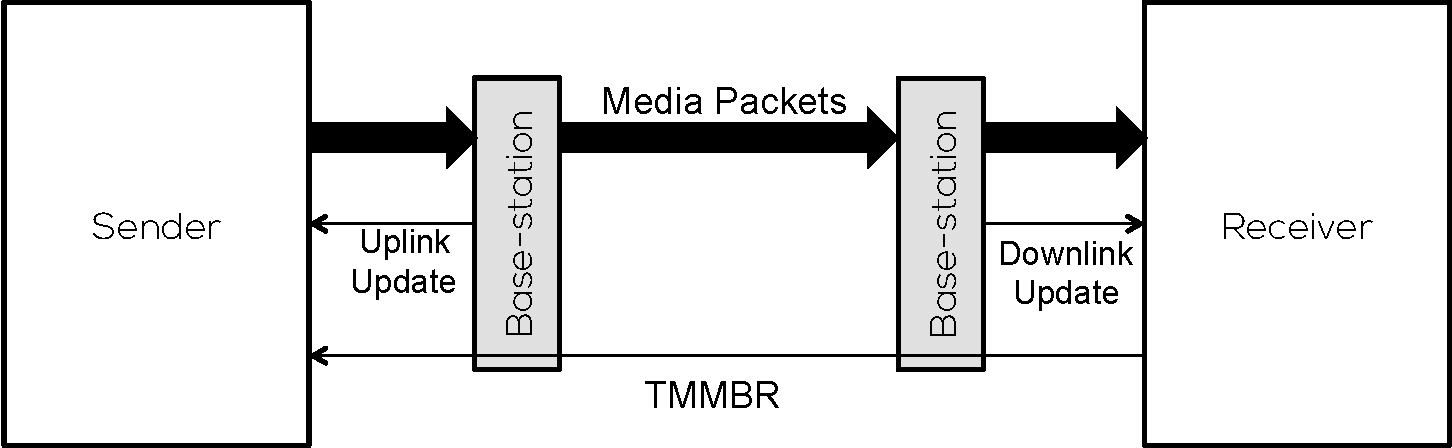
\includegraphics[width=\textwidth]{chap8-fig-tmmbr}
  \caption{Endpoints receiving capacity indication from the middleboxes
  (TMMBR) for implementing congestion control.}
\label{fig:cc:tmmbrab}
\end{figure}

In wireless networks, such as 3G/LTE, the last hop is typically the bottleneck
because the core network is well provisioned. In \citepub{c:3grc}, we
implement a network-assisted congestion control scheme wherein base-stations
(along the media path) notify the mobile terminals about the available link
capacity. In TMMBR-A, the base-stations notify both the sending and receiving
endpoints about the available capacity, i.e., the sender is notified about the
uplink capacity and the receiver is notified about the downlink capacity. If
an endpoint sends and receives data, it is notified asynchronously about the
uplink and downlink capacity. Figure~\ref{fig:cc:tmmbrab} shows a schematic
representation of the interaction between the middleboxes and the
endpoints. In TMMBR-B, the receiving endpoint is solely notified about the
downlink capacity. Both TMMBR-A and TMMBR-B employ a co-operative congestion
control scheme, wherein the receiver sends a TMMBR request to the sender
containing the current downlink capacity. In TMMBR-A, the sender also receives
a notification about the uplink capacity from the base-station; hence,
comparing the request from the receiver and the notification from the base-station, 
the sender chooses the minimum of the two values as the new target bit rate. In
TMMBR-B, the sender calculates the \emph{sender's estimate} (similar to the
one described in~\ref{cc:co-op}) and chooses the minimum of the sender's
estimate and the receiver's bit rate request. 


Figure~\ref{fig:tmmbn} shows the sample performance of TMMBR-A and TMMBR-B,
where both endpoints are sending media over a 3G network. TMMBR-A, due to its
knowledge about the network conditions at the uplink and the downlink, provides
an average throughput of 180\,\emph{Kbps} and 0\,\% loss, while TMMBR-B provides a
comparable throughput of 178\,\emph{Kbps} but with a 2\,\% loss ratio.

% Eventhough modern 3G/LTE networks are capable of providing these updates, they
% do not for several reasons

\begin{figure}
  \centerline{
    \subfloat[TMMBR-A]{
      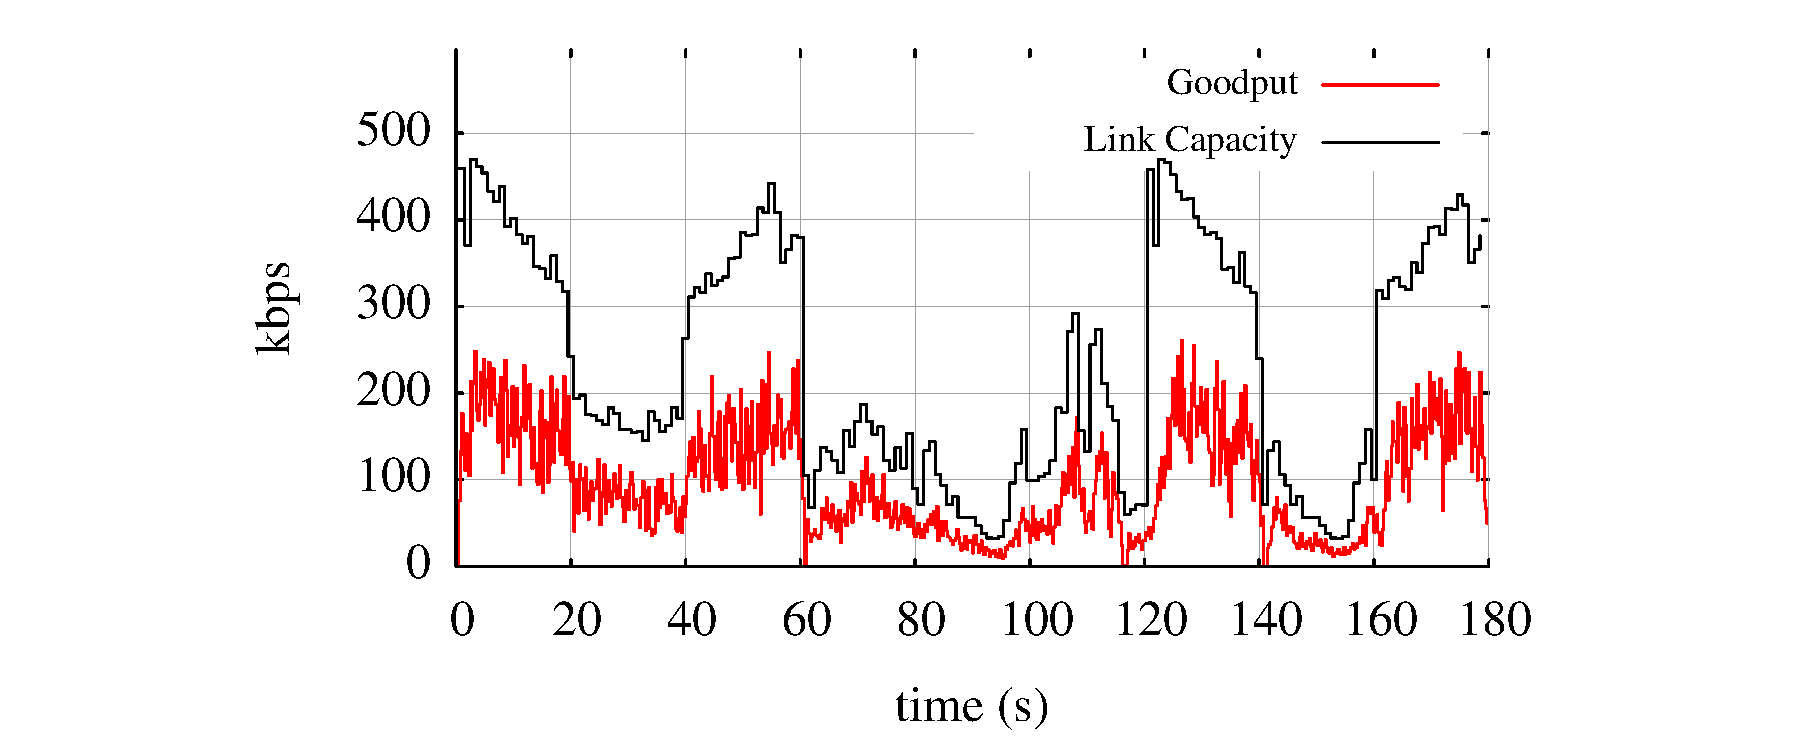
\includegraphics[width=0.5\textwidth, clip=true, trim=3cm 0 4.5cm 0]
      {chap8_graph_3g_tmmbr_a}
    }
    \subfloat[TMMBR-B]{
      \includegraphics[width=0.5\textwidth, clip=true, trim=3cm 0 4.5cm 0]
      {chap8_graph_3g_tmmbr_b}
    }
  }
  \caption{Performance of bandwidth indications by the base
  stations. a) TMMBR-A: both terminals are assisted, b) TMMBR-B: only the receiver
  is assisted.}
  \label{fig:tmmbn}
\end{figure}


\section{Off-path Congestion Cues}

% Congestion map

Modern mobile networks have been designed to carry multimedia streams with QoS
traffic classes~\cite{3gpp.23.107}, but deployments of GPRS, 3G and HSDPA
networks show that there are still geographical areas where best-effort
traffic classes are used~\cite{Curcio:glass, 6012045}. To overcome these challenges, in
\citepub{c:glass}, we implement a bandwidth coverage map that collects
connectivity information from the users (\emph {crowd-sourcing}) and
calculates the available capacity at the reported geographical locations.

Service Maps are presented in~\cite{1630563} and the measurement-based
approach is proposed in~\cite{Aravinda:2008p14}. GPS-based congestion control
is introduced in~\cite{Yao:2008p21}, and evaluated in different
scenarios (\cite{Yao:2009p57}, \cite{Yao:2010p64}), but they take signal
strength as an influential factor for rate-control and show that predicting
based on signal strength alone is insufficient. Yet, their results indicate
that past information can be used to predict future network characteristics.

\cite{6012045} proposes a similar architecture (\emph{bandwidth lookup
service}) to the one in \citepub{c:glass}, but uses different types of
averaging algorithms to predict future network characteristics in Dynamic
Adaptive Streaming over HTTP (DASH). While the averaging algorithm is not a
focus of this thesis, we use K-means~\cite{Kanungo:2002:LSA:513400.513402} and
K-nearest neighbor (K-NN)~\cite{Iwerks:2003:CKN:1315451.1315496} algorithms to
form regions with similar capacity. Details of the averaging algorithms
employed by our coverage map server are discussed in~\cite{sharmistha-thesis}.
A contrary approach is employed by \emph{Netradar.org}~\cite{6576402} which
divides the Earth's geographic map into 100m\,x\,100m squares. All measurements in a
specific area are averaged, and the maximum, minimum and mean values for 
each operator in that area is reported. 

\cite{Riiser:2012:2240136} proposes fetching the bandwidth along a travel
route in steps of 100 meters, which we find limiting. Instead, we propose
multiple methods for discovering areas with poor connectivity (e.g., known
travel route, area look ahead, geo-fencing or subscribing to coverage holes.)
and show that not only looking up future bandwidth but also when to vary the
sending rate affects the usefulness of the service. A preliminary analysis
using simulations of our system is done in~\cite{Curcio:glass}.

\begin{figure}
\includegraphics[width=0.9\textwidth]{chap8-fig-ecv}
  \caption{Endpoints using a Network Coverage Map Service to send coverage
  updates, query for upcoming congestion and receive coverage updates.}
\label{fig:cc:ecv}
\end{figure}

\begin{figure}
  \centerline{
    \subfloat[Map area lookahead]{
      \includegraphics[width=0.8\textwidth]
      {chap8-fig-ota-tr-net-02}
    }
  }
  \centerline{
    \subfloat[Known travel route Lookahead]{
      \includegraphics[width=0.8\textwidth]
      {chap8-graph_route_thin_throughput}
    }
  }
  \caption{a) A map of the available capacity around Otaniemi (university
  area). b) Example of the average and the Inter Quartile Range
  ($IQR=\pm1\sigma$) throughput along a known route. The data in both
  representations were captured over several days.}
  \label{fig:glass:map}
\end{figure}

In \citepub{c:glass}, we present a mechanism enabling an endpoint (usually a
receiver) to proactively react to upcoming capacity limitations in wireless
access networks. We enable this by implementing three steps,
Figure~\ref{fig:cc:ecv} shows the interaction between the endpoints and the
Network Coverage Map Server (NCMS). First, each endpoint receiving a media
stream monitors the throughput and its geolocation and reports it to the NCMS.
Figure~\ref{fig:glass:map} shows the throughput around the university area in
Espoo. Second, each endpoint is capable of querying the NCMS for upcoming
congestion (known as \emph{lookahead}). Using one of
the following methods: known travel route, area lookahead or by subscribing to
areas with poor coverage, typically using geo-fencing\footnote{Areas where the
expected channel capacity is lower than the media bit rate}.
Figure~\ref{fig:glass:map} shows a graphical representation of the average
throughput for an \emph{area lookahead} and a \emph{known travel route}. Third,
for each lookahead requests, the NCMS responds with an coverage map info,
i.e., the expected throughput at every geolocation along the route or
requested area.

The receiver uses these hints provided by the NCMS to implement congestion
control and sends an \emph{estimated capacity vector} (a data structure
containing a time-series of available throughput, thus preserving user's
location privacy) to the sender, which can alter the sending rate based on the
received information. The sender can use one of the following techniques to pick the
sending rate: 1) adapt the encoding rate, 2) perform a rate-switch, or, 3)
pre-buffer. Changing the encoding rate is only possible in interactive 
real-time media, because the RTP sender co-operates with the encoder to  modify the
encoding rate. Rate-switching is possible for streaming content  encoded at
different bit rates. It is also possible to use rate-switching  for
interactive real-time media involving scalable video codecs or simulcast
media, wherein a media stream is encoded at different bit rates and the
application switches between the stored media files. The performance of the
congestion control in this case depends on the granularity of the chosen bit
rates for the individual media streams. Lastly, varying the amount of 
pre-buffered video provides a more consistent experience to the user,  because the
technique attempts to maintain multimedia playback at a constant media
encoding rate. This is only applicable to stored content since the multimedia 
application typically reads ahead in the media stream and sends more data 
much before before it detects poor coverage.

In \citepub{c:glass}, video is sent from a server to mobile clients. The user
in the experiments mainly commuted around the city of Helsinki and Espoo using
public transport. The NCMS collected the measured throughput for each client;
thereafter, we conducted simulated experiments of users traveling at different
vehicular speeds through the Helsinki region. In total, the NCMS collected
over 400,000 updates over a month of operation (about 40-50 bus trips). The
NCMS received more than 10,000 updates for 6 geographical areas
(\emph{Otaniemi}, Helsinki City Center) while on average each geographical
location had around 100 updates.

In \citepub{c:glass}, we describe a scenario where a user moves smoothly
through a set of locations along a route and the receiver performs
\emph{lookahead} queries to fetch coverage information for surrounding areas.
In this scenario, there are gaps in coverage but overall the throughput at
most locations is above the required media rate. We analyse the performance of
four different algorithms: 1) the \emph{omniscient algorithm}, in which the
endpoint is aware of the exact end-to-end channel capacity and is expected to
perform the perfect rate-adaptation. 2) \emph{no adaptation}, in which the endpoints
perform no congestion control and the stream is transmitted at a constant bit
rate. In the periods when the link capacity falls below the media rate, the 
receiver will observe an increase in losses/discards, which may result in 
frequent pausing of the video. 3) \emph{Rate-switching}, in which the endpoints perform short
\emph{lookaheads}, which enables the endpoints to detect outages a few moments
before the user enters a location with poor connectivity. In this case, the
receiver sends a TMMBR message (with lowest available bit rate in the area)
before entering the area and another one after the exiting the area (to reset
the bit rate). The sender reacts by switching the media stream to the closest
available media rate. 4) \emph{Late scheduling}, in which the receiving endpoint
searches for areas with poor coverage much before the user arrives at those
locations, so that it can pre-buffer the content equivalent to the duration of
the disruption. To reduce the impact of changing routes, the streaming client
uses the congestion control algorithm proposed in \citepub{c:glass}.

\begin{table}
  \begin{center}
\begin{tabular}{ccccccc} \hline
Method & $SR_{avg}$ & $PSNR_{avg}$ & $\sigma_{PSNR}$ & PLR \\ \hline
% & $buffer_{max}$\\ \hline
No adaptation   & 865   & 27.48 & 4.55  & 6.6 \\
Omniscient      & 929   & 43.12 & 1.9   & 0.33 \\ 
Rate-switching  & 881   & 42.75 & 2.21  & 0.0  \\ 
Late scheduling & 1014  & 48.43 & 0.18 & 0.0  \\ \hline
\end{tabular}
\caption{A bus ride with good 3G coverage.}
\label{table-glass-sim7res}
\end{center}
\end{table}


Table~\ref{table-glass-sim7res} compares the results for the different schemes
and Figure~\ref{fig:glass:sim7res} shows the sending/receiver rate variation
to channel throughput for one out of 10, simulation runs. The \emph{omniscient
algorithm} provides the best rate-adaptation but since it is unable to 
pre-buffer, the PSNR ($PSNR_{avg}$=43) is lower than that of late scheduling
($PSNR_{avg}$=48). Alternatively, performing \emph{no adaptation} causes
frequent pausing when the capacity is lower than the media rate, additionally,
packet loss also affects the media quality and is reflected in the low PSNR
($PSNR_{avg}$=27). \emph{Rate-switching} has comparable results to the
\emph{omniscient} case because it avoids congestion by switching to bit rates
lower than the minimum reported throughput. There are no losses and the average
PSNR is 42.75, which is comparable to the \emph{omniscient} case. \emph{Late
scheduling} outperforms the rest of the schemes in terms of media quality
(measured in terms of average PSNR, $PSNR_{avg}$=48.43) mainly because it
attempts to stream media at a single quality level; it relies heavily on 
pre-buffering, constantly updating the size of the pre-buffer to compensate for
the longest disruption it finds along the travel-route or in the viscinity of
the user. Another reason is that, in our measurements, we found low density of
poor coverage areas and good connectivity in areas in between, allowing the
client to pre-buffer content. However, when it is not possible to pre-buffer,
the client will perform a rate-switch. Finally, we expect the performance of
the congestion control to be at least that of rate-switching because the
sender will be able to vary the sending rate preemptively without probing.

\begin{figure}
\includegraphics[width=0.9\textwidth]{chap8-graph-sim7-3}
  \caption{The plot shows the variation of sending rate to 3G link capacity
  based on a) no adaptation b) Omniscient c) Rate-switching d) Late scheduling
  when there are few coverage holes and good connectivity between them.}
\label{fig:glass:sim7res}
\end{figure}


We find that the information provided by the NCMS is suitable for both
predictive rate-switching and  pre-buffering and helped in avoiding almost all
packet losses in the scenarios we investigated, noticeably increasing video
quality. This system works for video streaming and can be adapted for
interactive media communication, wherein the sender employs a co-operative
congestion control scheme, i.e., the sender receives the \emph{estimated
capacity vector} from the receiver and \emph{coverage map information} for
itself from the NCMS; it then picks the minimum of the two rates and implements any
additional rate recommended by the congestion control (one of the algorithms
discussed in Chapter~\ref{chap:cc}).

\section{Summary}

In this chapter, we describe two congestion control mechanisms that both use 
out-of-band signaling, but use in-path and off-path sources, respectively. First,
the in-path sources is based on receiving congestion cues from middleboxes
(e.g., 3G or LTE base-stations) and uses standard RTP extensions (e.g., TMMBR)
for signaling. Second, the off-path source is a crowd-sourced 3G coverage
map that collects throughput and geolocation information from users and then
notifies the subscribed endpoints about the available capacity in their
respective neighborhoods. We propose a system to collect and query coverage
maps. The endpoints query the coverage server using out-of-band signaling to
discover areas of poor coverage; based on these notifications the endpoints
vary their sending rate.

We show that notification from middleboxes such as base stations would
help endpoints perform better congestion control, in for example, mobile network. 
When an LTE cell is experiencing extreme load\footnote{Extreme load
occurs when an LTE cell has about 10x more users than when it is busy.}.
Furthermore, we also show that using congestion maps also aids in performing
congestion control. A congestion map is a measurement service that aggregates
throughput information from multiple users and sends notification of areas
with poor coverage to its subscribers. We expect these notifications to be
used as congestion cues and not as a replacement to in-band, in-path
congestion control. The main reason for restricting the use of such a service
to notify congestion cues is that such a service is vulnerable to data
pollution, i.e., the clients may report incorrect measurements, not
necessarily intentionally but because of programming errors. Another reason is
that, in the reported notifications may depend on the way the aggregation is
performed and how quickly the aggregation converges to the prevailing network
conditions in a region. A fast convergence may be susceptible to misreporting,
leading to false positives and causing the user experience to fluctuate when in
reality there would be no reason for it to fluctuate. A slow convergence would
ignore minor spikes in load and endpoints would experience a poor quality of
experience for a brief period until the values converge. A slow convergence
may also lead to inefficiency because once an aggregation value in a region
drops, it would stay there unless the endpoints probe for additional capacity.

While we show that NCMS can be used for streaming both the live and stored
multimedia content, it can be adapted to work with interactive media services.
However, we believe that the NCMS notifications would perform best when
working alongside an existing congestion control algorithm.


\chapter{Conclusions}
\label{chap:conc}
 In this thesis, we have described our proposed classification of congestion
control cues (framework) in Chapter \ref{chap:cc.fw}. When discussing the
different parts of the framework, we highlighted the existing related work and
our contributions in those areas. In terms of innovativeness, the congestion
control framework provides options to look at congestion cues beyond those
reported by the receiver in an RTCP Receiver Report. The framework allows the
congestion control algorithm to use multiple paths for either aggregating
capacity or for increasing error-resilience, or to use capacity notifications from
middleboxes along the path, or to build a coverage map that provides
congestion notification as a third-party services. Each of these techniques
apply to one of the four areas described in the framework; however, the
definitions of each area are generalised enough to allow the application of a
broad range of techniques, not just those proposed in this thesis.

% insights and criticism

We defined a new class of co-operative congestion control algorithms and
believe that these algorithms will replace the purely sender-driven
mechanisms currently in use. 
The reason is that the co-operative algorithm lets the receiver
not only measure the end-to-end capacity but assess the quality of experience
(rendering quality) to decide its rate estimate. As with the 
sender-driven approach, the sender estimates the congestion based on the reported
cues and its current sending rate, but the sender can then factor in the
receiver's estimate before finally choosing a new target bit rate. We already
see an uptake of this general idea, with Google’s proposal for multimedia
congestion control in WebRTC~\cite{draft.rrtcc}.

Another observation that we made during our research was that many multimedia
systems implement the error-resilience and congestion control algorithms
separately. We believe the community has not explored the use of FEC for congestion
control in depth, partly because interactive multimedia flows have very tight
delay constraints and FEC may not arrive in time for recovering the lost
packet. The results outlined in this thesis show that FEC can be used for
congestion control and perform suitably when no bursty loss occurs.

\begin{figure}
    \centerline{
        {\includegraphics[width=\textwidth] %clip=true, trim=0 1cm 0 1.5cm]
        {chap9-fig-all-tech}}
    }
    \caption{Interworking of all the ideas presented in this thesis.}
    \label{chap9:all_in}
\end{figure}

\section{Synthesis}

While the techniques proposed in this thesis were only shown to work
independently, nothing prevents them from interworking.
Figure~\ref{chap9:all_in} depicts an example for a comprehensive architecture
wherein an endpoint will be able to use cues from all the above sources to
perform multimedia congestion control and packet scheduling. Endpoints will
always use the multipath extensions for RTP (MPRTP), even when using a single
path; this will allow the opportunity to offload or aggregate capacity when
new interfaces (or paths) appear (Block A of Figure~\ref{chap9:all_in}).

Since the circuit breaker algorithm relies on basic congestion cues (RTT and
loss) and periodic reception of RTP and RTCP, the circuit breaker sets the
boundary condition under which all future multimedia application will operate.
The congestion control will not just rely on the cues reported in an RTCP
RR/XRs, but gather hints from additional sources. For instance, mobile base
stations can help provide information whenever capacity allocation changes due
to mobility, an increase in active users, or handovers (Block B of
Figure~\ref{chap9:all_in}). Enabling Explicit Congestion Notification (ECN) in
the network and getting ECN-marked packets is another way of enabling
collaboration between the network and the endpoints. Lastly, using network
coverage maps to get information about prevailing network conditions would
also assist in congestion control (Block C of Figure~\ref{chap9:all_in}).
The main concern in this case is to ascertain the trustworthiness and
reliability of the indicated measurement values. Since the additional
congestion cues are just hints and part of a larger set of cues, an endpoint
may ignore cues that seem erroneous or provide false indication than the other
cues. 

% The recent disclosures of pervasive active monitoring has caused many services
% to take security more seriously. This has resulted in turning on encryption.
% Activating encryption means that middleboxes, which peeked into the traffic to
% provide differentiated quality of service, are now unable to do that anymore.

These additional hints are also essential at session
startup, because currently a media application typically starts sending media
at a pre-configured value (either set very low or set to the maximum media
rate). Receiving notifications from a NCMS server at the beginning of the
session may help the endpoint pick a better start rate.


Block D of Figure~\ref{chap9:all_in} shows that the receiver sends an RTCP
RR and XR containing typical congestion cues. It also sends any estimate made
by a receiver-side congestion control algorithm (e.g., using TMMBR, REMB).
Furthermore, it adds any throughput notifications it may have received from an
on-path middlebox (RTCP XR containing ECN markings or capacity changes
indicated by a base station) or from a NCMS server. The sender decides the new
target bit rate based on the congestion cues reported by the receiver, and the
notifications it has also been receiving from an on-path middlebox or from the
NCMS (Block E of Figure~\ref{chap9:all_in}).


Finally, depending on the underlying codec implementation, the new target rate
may result in: a change in the encoding rate of an audio and/or video stream,
a change in the number of layers produced by a Scalable Video Codec (SVC),
packetization time (ptime) of an audio stream, or a change in the number of
simulcast multimedia streams (typically video streams).

\section{Future Directions}

Another aspect of MPRTP that is not discussed in detail in this thesis is the
role of MPRTP in overlay networks, or for processing media in data centers. Very
large conferences, with hundreds of participants can be arranged in complex
topologies containing combinations of cascaded meshes and trees. Such very
large media conferences (e.g., massive open online courses, seminars or
conferences), usually have a low peer churn because all participants arrive
and leave roughly at the same time. Also, the active participants produce the
media flows, while the dormant/passive participants consume it and occasionally
chime in with questions and comments. Instead of broadcasting to all the
participants, which may create load on a centralised server and require
scaling, we can exploit the asymmetric relationship between the participants
by using them as overlays. This would require participants to forward at least
as much as they receive, if not more, and using multiple paths eases this
requirement~\cite{Noh2008,Li2010a,Globisch:AsymGrpComm}.


% \section{Future Work}

% For each of the proposed congestion control techniques in this thesis, we make
% deployment recommendations and for some of these techniques the deployment
% considerations overlap. 

In the near-term, we see the following elements of emerging. First,
the emergence of WebRTC requires standardised congestion control.
Chapters~\ref{chap:cc} and~\ref{chap:er-cc} make some proposals that may fit
this purpose, but it requires more extensive evaluations to be deployment-ready.
Second, using FEC for congestion control needs to be generalised to work with
any other multimedia congestion control algorithm, to enhance the
applicability of the congestion control. Third, multipath scheduling needs to be reconsidered for
interactive multimedia communication. One way of achieving this would require
implementing a coupled congestion control that synthesises all the subflow
cues to arrive at an overall rate that would fit the combined paths and then
let the current scheduling algorithm allocate the bits per subflow. Fourth,
the scalability and robustness of the network coverage map service needs to
studied; furthermore, the location-throughput matching algorithm needs to be
studied in more detail to respond to diverse reporting from
various mobile devices, etc. Lastly, all these techniques need to be combined for
implementing a unified congestion control for interactive multimedia .



% Various conference architectures can be used to distribute the media in a
% many-to-many communication scenario: centralized, unicast receive with
% multicast send, full mesh, overlays, and trees
% \cite{Li2010a,Noh2008,Singh2001}. When developing a conferencing systems for a
% specific use-case, the scalability, reliability, quality and delay
% characteristic, for each of architecture needs to be considered. In the case
% of of very large video conferences, such as, massive open online course,
% seminars or conferences, we assume a low peer churn i.e., all participants
% arrive and leave roughly at the same time. Also, active participants produce
% the media flows, while the dormant/passive participant consume it. In
% \cite{Globisch:AsymGrpComm}, we propose using multiple Application Layer
% Multicast (ALM) distribution trees to broadcast the media from an active
% speaker to the participants listening in to the conference. The ALM tree
% network minimizes the end-to-end delay and reduces the load on the active
% participants.

% The use of multiple Application Layer Multicast (ALM) trees for media delivery
% minimizes the end-to-end delay and results in asymmetric relationships between
% participants and introduces complex forwarding. Chu \emph{et al.} show ALM as
% a viable solution for real-time conferencing over the Internet~\cite{Chu2001}.
% Banerjee et al.\cite{Banerjee2002} present an ALM protocol that has a
% hierarchical control structure with low overhead. Noh \emph{et
% al.}~\cite{Noh2008} use multiple trees to reduce the end-to-end delay and
% determine the optimal number of ALM trees depending on specific network
% characteristics. They conclude that the fan-out of a peer influences the
% trade-off between the propagation delay and the queuing delay. Li et
% al.~\cite{Li2010a} describes the use of multiple trees as a mechanism to scale
% to more clients by introducing multiple focus-mixer structures where each
% structure is dedicated to serving a set of clients in a region.

% In \cite{draft.rtcp.overlay}, instead of using a centralized conferencing
% server to maintain the media sessions and inserting peers or nodes in the
% appropriate location, we propose protocol extensions (e.g., to RTCP) to help
% nodes re-arrange themselves based on their pairwise connectivity, i.e.,
% reconstructing the tree by preferring links with better network
% characteristics.

%%%%%%%%%%%%%%%%%%%%%%%%%%%%%%%%%%%%%%%%%%%%%%%%%%%%%%%%%%%%%%%%%%%%%%%%%%%%%%

%% The following commands are for article dissertations, remove them if you
%% write a monograph dissertation.

% Errata list, if you have errors in the publications.
%\errata

%%%%%%%%%%%%%%%%%%%%%%%%%%%%%%%%%%%%%%%%%%%%%%%%%%%%%%%%%%%%%%%%%%%%%%%%%%%%%%

%% The first publication (journal article)
% Set the publication information.
% This command musts to be the first!

\addpublication[conference]{V. Singh, S. McQuistin, M. Ellis, C.
Perkins}{Circuit Breakers for Multimedia Congestion Control}{IEEE Packet
Video}{San Jose, USA}{Dec}{2013}{IEEE}{c:cb}

% Add the dissertation author's contribution to that publication.

\addcontribution{The author of this dissertation was the main author of this
paper~\cite{Singh:CB.eval}. His contribution consisted of implementing the
algorithms and conducting experiments in one of the two evaluation scenarios
discussed in the paper.}

% Add the errata of the publication, remove if there are none (the order can
% be interchanged with \addauthorscontribution).
%\adderrata{This is wrong}
% Add the publication pdf file, the filename is the parameter (must be the
% last).

% \addpublicationpdf{add/9_cb.pdf}

%%%%%%%%%%%%%%%%%%%%%%%%%%%%%%%%%%%%%%%%%%%%%%%%%%%%%%%%%%%%%%%%%%%%%%%%%%%%%%

%% The second publication (conference article, note the optional parameter)
% Set the publication information.

\addpublication[conference]{V.Singh, J. Ott, I. D. D. Curcio}{Rate adaptation
for 3G Conversational Video}{IEEE Infocom Workshops}{Rio de Janeiro,
Brazil}{04}{2009}{IEEE}{c:3grc}

% Add the dissertation author's contribution to that publication.

\addcontribution{The author of this dissertation was the main author of the
paper~\cite{Singh:3gRC}. His contribution consisted of implementing the system
and analyzing the results.}

% \addpublicationpdf{add/2_3g_ra.pdf}

%%%%%%%%%%%%%%%%%%%%%%%%%%%%%%%%%%%%%%%%%%%%%%%%%%%%%%%%%%%%%%%%%%%%%%%%%%%%%%

%% The third publication (another journal paper, accepted for publication,
%% note the optional parameter)
% Set the publication information, detailed information can be empty

\addpublication[conference]{V. Singh, J. Ott, I. D. D. Curcio}{Rate Adaption
for Conversational Video in Heterogeneous Environments}{IEEE World of
Wireless, Mobile and Multimedia (WoWMoM)}{San Francisco,
USA}{06}{2012}{IEEE}{c:hetrc}

% Add the dissertation author's contribution to that publication.

\addcontribution{The author of this dissertation was the main author of the
paper~\cite{Singh:HetRC}. His contribution consisted of implementing the
system and analyzing the results.}

% \addpublicationpdf{add/3_het_ra.pdf}

%%%%%%%%%%%%%%%%%%%%%%%%%%%%%%%%%%%%%%%%%%%%%%%%%%%%%%%%%%%%%%%%%%%%%%%%%%%%%%

\addpublication[conference]{V. Singh, A. A. Lozano, J. Ott}{Performance
Analysis of Receive-Side Real-Time Congestion Control for WebRTC}{IEEE Packet
Video}{San Jose, USA}{Dec}{2013}{IEEE}{c:eval}

% Add the dissertation author's contribution to that publication.

\addcontribution{The author of this dissertation was the main author of this
paper~\cite{Singh:rrtcc.eval}. His contribution consisted of designing the
experiments and analyzing the results discussed in the paper.}

% \addpublicationpdf{add/10_rrtcc.pdf}

%%%%%%%%%%%%%%%%%%%%%%%%%%%%%%%%%%%%%%%%%%%%%%%%%%%%%%%%%%%%%%%%%%%%%%%%%%%%%%

\addpublication[conference]{Devadoss J., Singh V., Liu C., Ott J., Wang Y-K.,
Curcio I.}{Evaluation of Error Resilience Mechanisms for 3G Conversational
Video}{IEEE ISM}{Berkley, USA}{Dec}{2008}{IEEE}{c:err}

% Add the dissertation author's contribution to that publication (the order
% can be interchanged with \adderrata).

\addcontribution{The author of this dissertation was one of the co-authors of
the paper~\cite{Devadoss:3gErr}. His contribution consisted of providing 2 out
of the 4 ideas discussed in the paper, implementing the corresponding
algorithms, providing the configurations for the experiments and co-editing
the paper.}

% \addpublicationpdf{add/1_3g_er.pdf}

%%%%%%%%%%%%%%%%%%%%%%%%%%%%%%%%%%%%%%%%%%%%%%%%%%%%%%%%%%%%%%%%%%%%%%%%%%%%%%

\addpublication[submitted]{M. Nagy, V. Singh, J. Ott, L. Eggert}{Rate-control
using FEC for Interactive Multimedia Communication}{---}{}{}{2013}{}{c:fecrc}

% Add the dissertation author's contribution to that publication.

\addcontribution{The author of this dissertation was one of the co-authors of
the paper~\cite{Singh:FECRC}. His contribution consisted of discussing the main
idea for the paper with the lead author, implementing the comparative algorithms, 
providing the configurations for the experiments and co-editing the paper.}

% \addpublicationpdf{add/6_fec_ra.pdf}

%%%%%%%%%%%%%%%%%%%%%%%%%%%%%%%%%%%%%%%%%%%%%%%%%%%%%%%%%%%%%%%%%%%%%%%%%%%%%%

\addpublication[conference]{V. Singh, S. Ahsan, J. Ott}{MPRTP: Multipath
Considerations for Real-time Media}{ACM Multimedia Systems (MMSys)}{Oslo,
Norway}{02}{2013}{ACM}{c:mprtp}

% Add the dissertation author's contribution to that publication.

\addcontribution{The author of this dissertation was the main author of the
paper~\cite{Singh:MPRTP}. His contribution consisted of providing the main
idea for the paper, providing the configurations for the experiments,
performing the statistical analysis, and acting as the main editor of the
paper.}

% \addpublicationpdf{add/5_mprtp.pdf}

%%%%%%%%%%%%%%%%%%%%%%%%%%%%%%%%%%%%%%%%%%%%%%%%%%%%%%%%%%%%%%%%%%%%%%%%%%%%%%

%% The fourth publication (yet another journal paper, submitted for
%% publication, note the optional parameter) Note that you are allowed to use
%% this option only when submitting the dissertation for pre-examination!
% Set the publication information, detailed information is not printed

\addpublication[conference]{V. Singh, J. Ott, I. D. D. Curcio}{Predictive
Buffering for Streaming Video in 3G Networks}{IEEE World of Wireless, Mobile
and Multimedia (WoWMoM)}{San Francisco, USA}{06}{2012}{IEEE}{c:glass}

% Add the dissertation author's contribution to that publication.

\addcontribution{The author of this dissertation was the main author of the
paper~\cite{Singh:Glass}. His contribution consisted of implementing the
system and analyzing the results.}

% \addpublicationpdf{add/4_glass.pdf}

%%%%%%%%%%%%%%%%%%%%%%%%%%%%%%%%%%%%%%%%%%%%%%%%%%%%%%%%%%%%%%%%%%%%%%%%%%%%%%

%\bibliographystyle{IEEEtran} %plain, amsalpha

\bibliographystyle{plain}

% argument is your BibTeX string definitions and bibliography database(s)
%\bibliography{IEEEabrv,../allpapers}

\bibliography{bib/diss,bib/rfc}

\end{document}
